%%    _____  _____
%%   |  __ \|  __ \    AUTHOR: Pedro Rivero
%%   | |__) | |__) |   ---------------------------------
%%   |  ___/|  _  /    DATE: June 20, 2020
%%   | |    | | \ \    ---------------------------------
%%   |_|    |_|  \_\   https://github.com/pedrorrivero
%%

\documentclass[9pt, aspectratio=169]{beamer}
% \documentclass[9pt, handout, aspectratio=169]{beamer}	% Skip \pause commands
\usetheme{PRRwide}
\usepackage{PRRmath}

% \setbeameroption{show notes}
% \setbeameroption{show only notes}

%% ----------------------------------------------------------------------------
%% FRONT-MATTER
%% ----------------------------------------------------------------------------

\title{Quantum Computation for the Understanding of Mass}
\subtitle{Simulating Quantum Field Theories}
\author{Pedro Rivero}
\institute{Illinois Institute of Technology \\ Argonne National Laboratory}
\newcommand{\mail}{priveroramirez@anl.gov}
\date{\today}
\newcommand{\website}{
	\href{https://www.phy.anl.gov}
	{www.phy.anl.gov}
}

\begin{document}
	\justify
	\setlength{\abovedisplayskip}{0pt}
	\setlength{\belowdisplayskip}{12pt}
	\setlength{\abovedisplayshortskip}{0pt}
	\setlength{\belowdisplayshortskip}{12pt}

\begin{frame}[plain,t]
	\titlepage
\end{frame}

\begin{frame}[c]{Contents}
%		\begin{multicols}{2}
%  			\tableofcontents
%		\end{multicols}
	\tableofcontents
\end{frame}


%% ----------------------------------------------------------------------------
%% MAIN-MATTER
%% ----------------------------------------------------------------------------

\section{Introduction}

\begin{frame}{Introduction}

	\begin{multicols}{2}

		\begin{itemize}
			\item<2-> Quantum Chromodynamics (QCD) is the theory of the strong nuclear force, and it holds many mysteries such as \textbf{mass generation}.
			\item<2-> QCD is currently studied using brute-force numerics on the world’s largest supercomputers, although many of its aspects cannot be reproduced by classical means.
			\item<3-> The \textbf{NJL model} is an effective field theory regarded as a low-energy approximation to QCD. It retains certain key features like the so called Goldstone modes, and \textbf{dynamical chiral symmetry breaking}; and can also be solved nonperturbatively for verification.
		\end{itemize}

		\begin{center}
			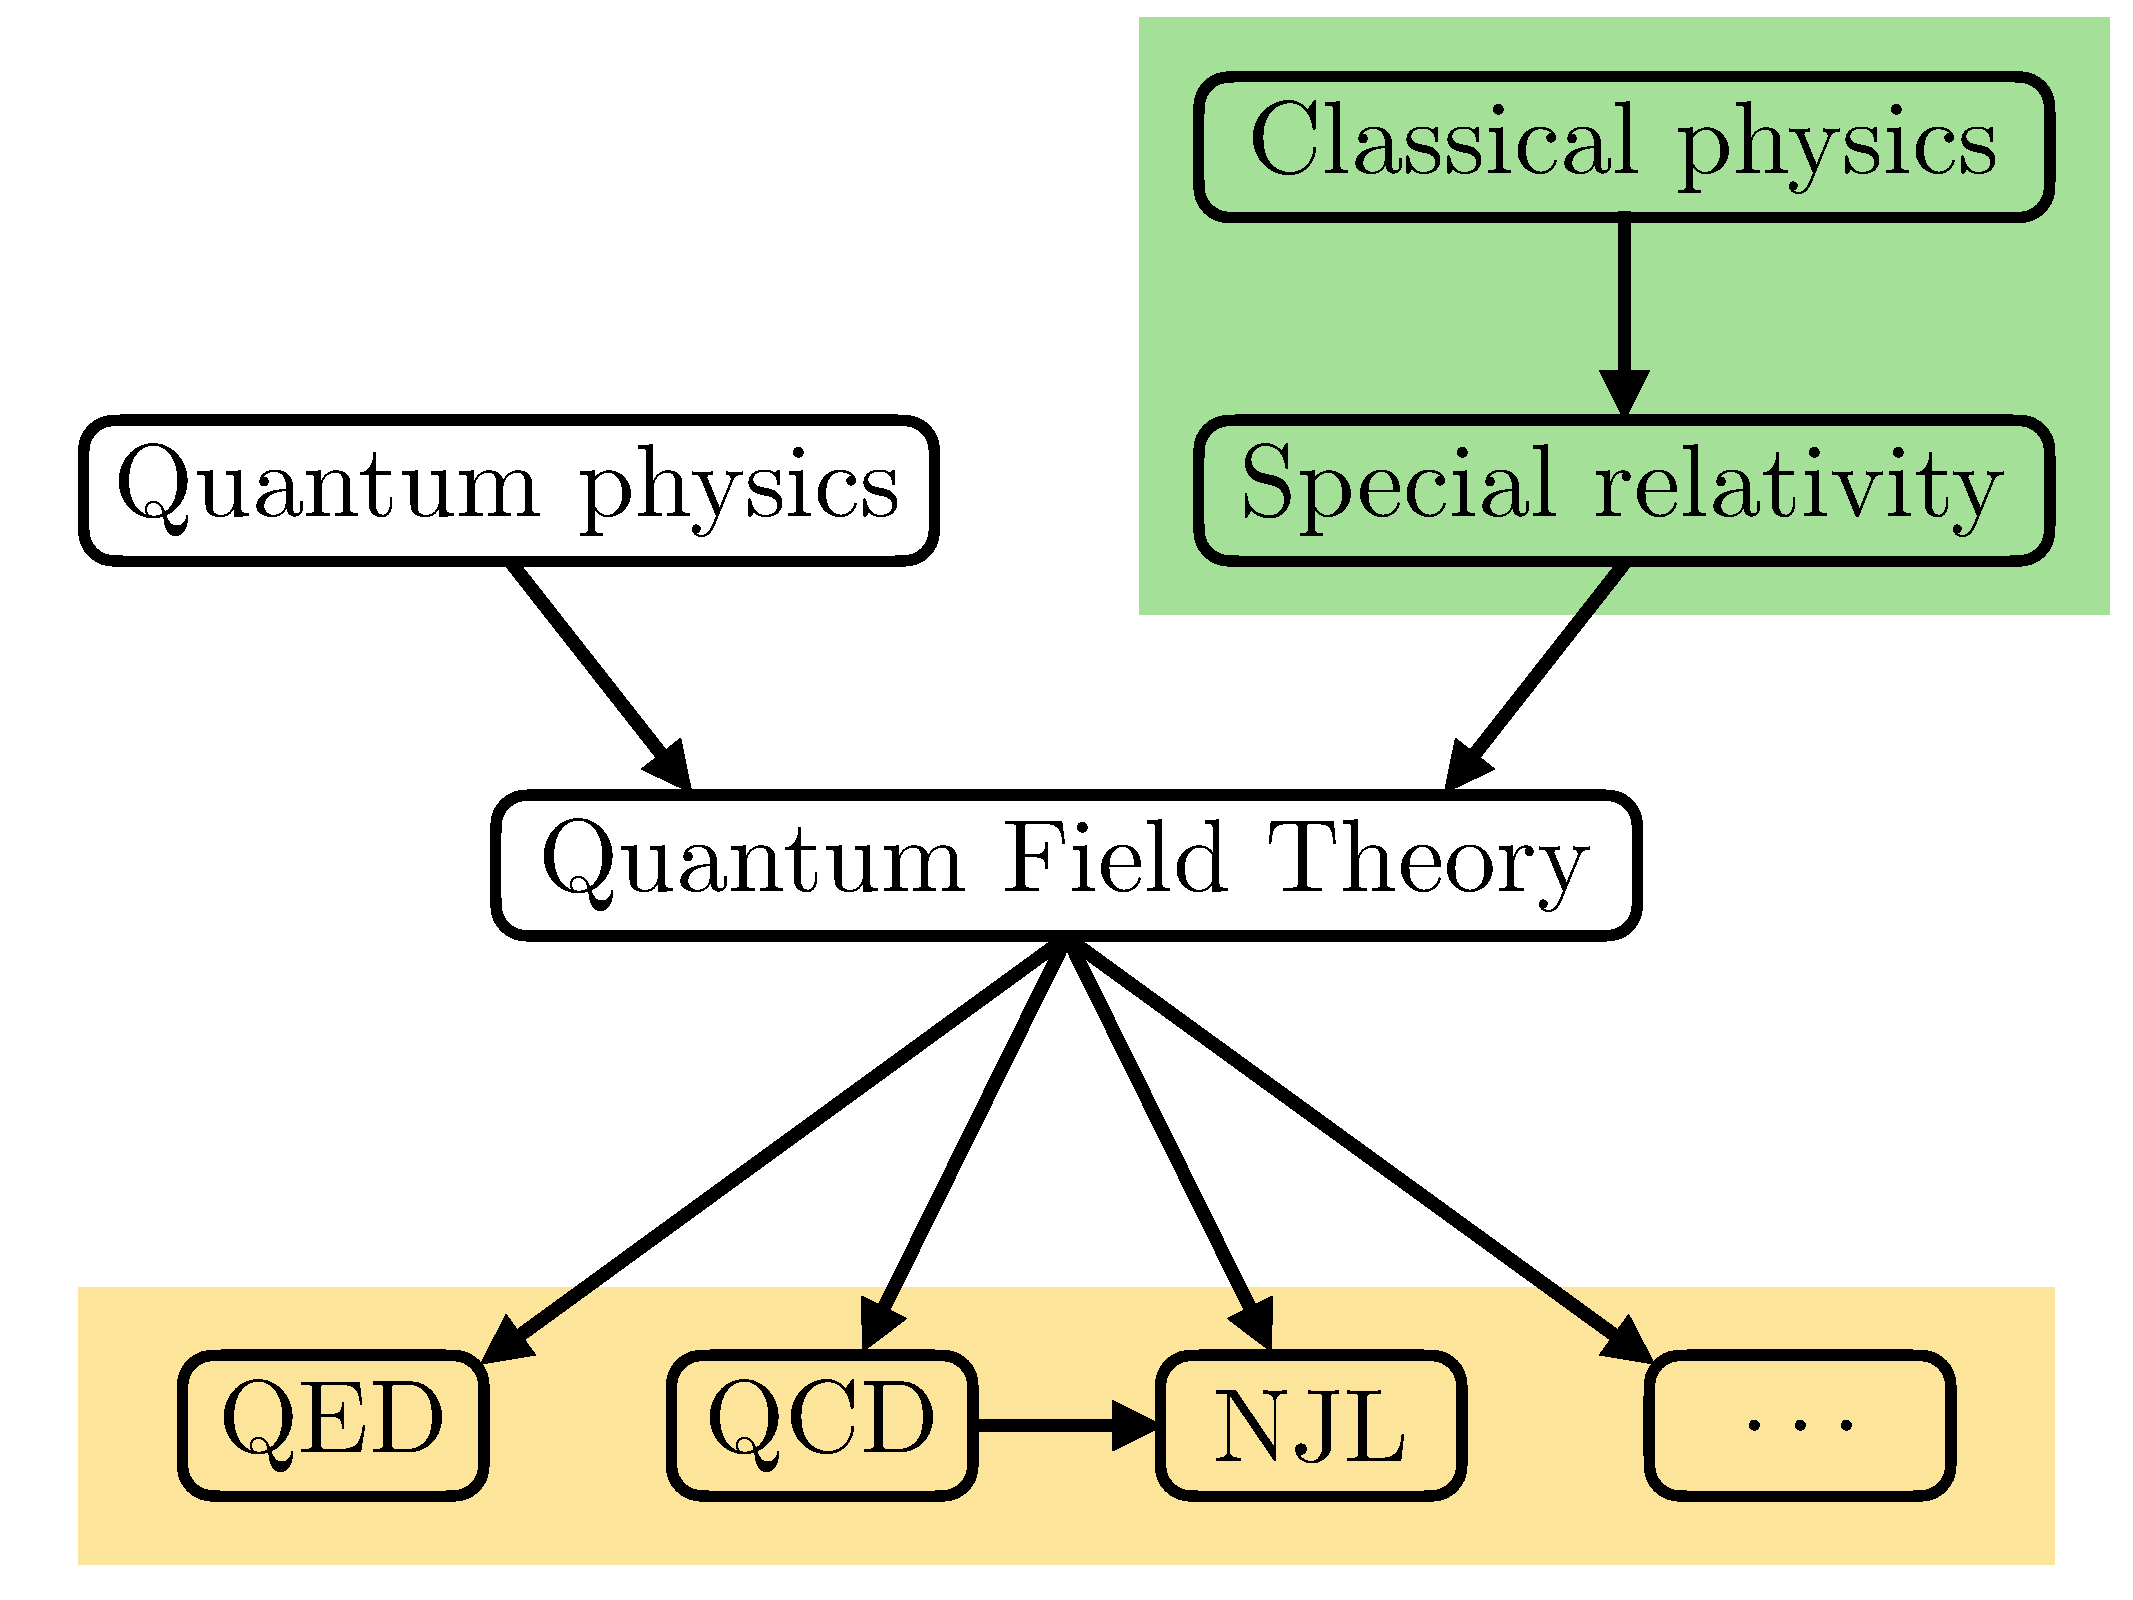
\includegraphics[width=.40\paperwidth]{Figures/quantum-field-theory}
		\end{center}

	\end{multicols}

\end{frame}

%% ----------------------------------------------------------------------------

% \begin{frame}[c]{Contents}
% %		\begin{multicols}{2}
% %  			\tableofcontents
% %		\end{multicols}
% 	\tableofcontents
% \end{frame}

%% ----------------------------------------------------------------------------
%% ----------------------------------------------------------------------------

\section{Solving the NJL model in $1+1$ dimensions}

\begin{frame}{Solving the NJL model in $1+1$ dimensions}

	\begin{multicols}{2}

		\begin{center}
			\underline{\textbf{NJL LAGRANGIAN DENSITY}}\\
			\small{\emph{Simplest version that reproduces a condensate}}
			\begin{gather*}
				\mathcal{L}(x) \defeq
			    \bar{\psi}(x) \qty(i\slashed{\partial}-m) \psi(x) + \mathcal{L}_{I}(x) \\[10pt]
				\mathcal{L}_{I}(x) =
			    \frac{1}{2} G_{\pi} \qty[\bar{\psi}(x)\psi(x)]^2
			\end{gather*}
		\end{center}

		\columnbreak

		\begin{center}
			\underline{\textbf{NJL HAMILTONIAN DENSITY}}\\
			\small{\emph{Obtained through the Lengendre transform}}
			\begin{align*}
			  \mathcal{H} &\defeq
			    \fdv{\mathcal{L}}{\qty(\partial_{0} \psi)} \qty(\partial_{0} \psi) +
			    \qty(\partial_{0} \bar{\psi})
			    \fdv{\mathcal{L}}{\qty(\partial_{0} \bar{\psi})} -
			    \mathcal{L} \\
			  &= \bar{\psi}(x)\qty(m - i\gamma^{1}\partial_{1})\psi(x) -
		    	\frac{1}{2} G_{\pi} \qty[\bar{\psi}(x)\psi(x)]^{2}
			\end{align*}
		\end{center}

	\end{multicols}

	\vspace{1em} \pause

	The \textbf{bare and dressed masses} appear on the bare quark propagator $S_{0}$, and the NJL dressed quark propagator $S$ respectively. We can find a relationship between these two by solving the \textbf{gap equation}:

	\begin{gather*}
		S^{-1} =
			S_{0}^{-1} - 2iG_{\pi} \int \frac{\dd[2]{p}}{\qty(2\pi)^{2}}
			N_\text{color} N_\text{flavor} \text{Tr}_\text{\tiny{D}}\qty[S] \\
	  M \simeq
	    m + 4iG_\pi N_\text{color} N_\text{flavor}
	    \int \frac{\dd[2]{p}}{(2\pi)^2} \frac{M}{p^2 - M^2}
	\end{gather*}

\end{frame}

%% ----------------------------------------------------------------------------

\subsection{Analytical solution}

\begin{frame}{Mass generation}

	\begin{center}
		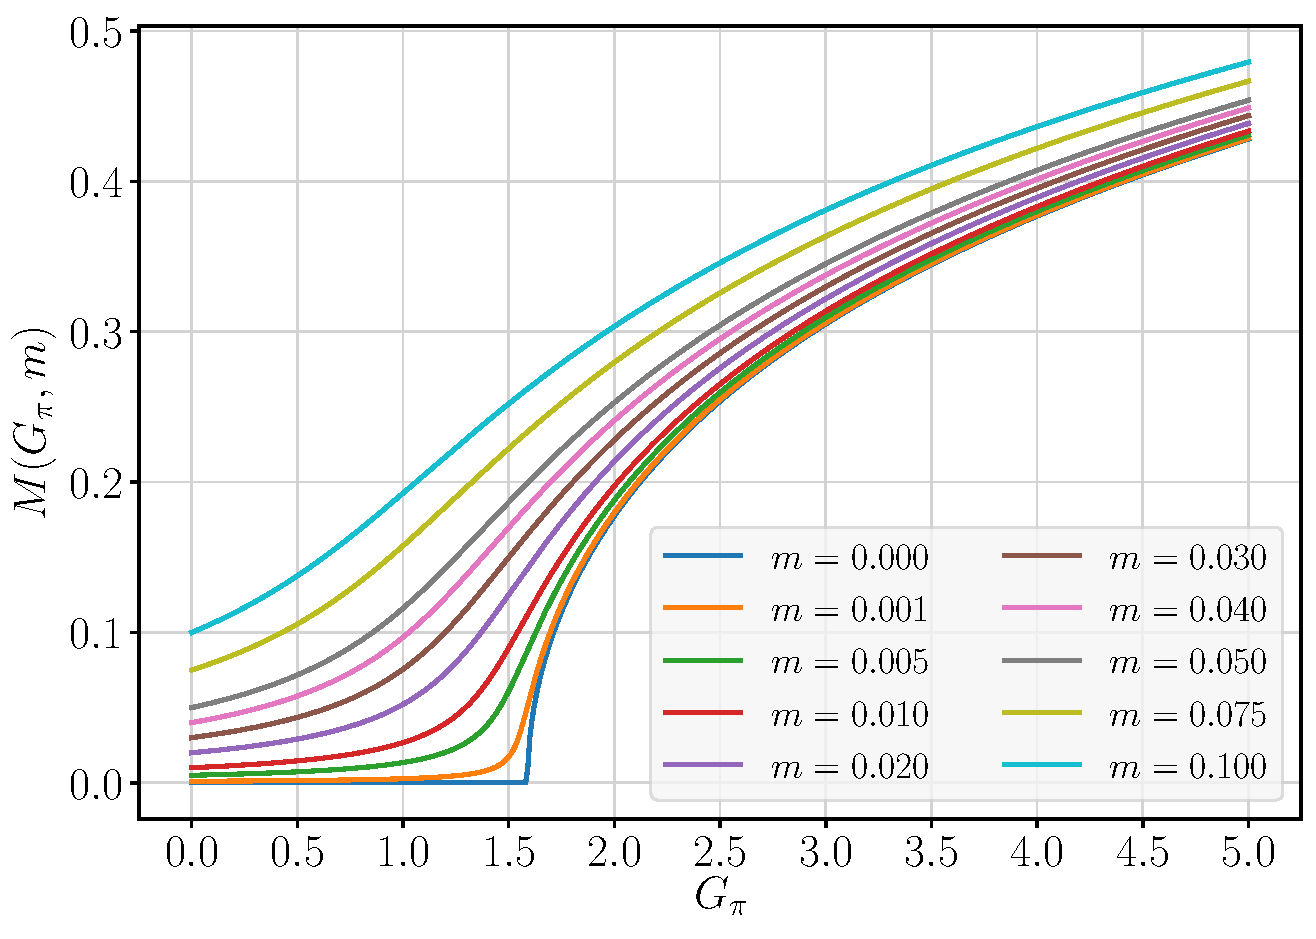
\includegraphics[width=.5\paperwidth]{Figures/NJL1-model-solving/NJL1-dressed-mass-curves}
	\end{center}

	\vspace{-1em}

	\begin{table}[!bp]
	  \centering
	  % \caption{Parameters used for solving the NJL model in $1+1$ dimensions.}
	  \label{tab:NJL1-analytical-solution-parameters}
	  \begin{tabular}{ c c c c c }
	    \hline
	    % \rule{0pt}{14pt}
	    $N_\text{Dirac}$ & $N_\text{color}$ & $N_\text{flavor}$ &
	    $\Lambda_{IR}$ & $\Lambda_{UV}$ \\
	    \hline
	    \hline
	    % \rule{0pt}{14pt}
	    $1+1 \ra 2$ & $1$ & $1$ & $0.240$ GeV & $0.645$ GeV \\
	    \hline
	  \end{tabular}
	\end{table}

\end{frame}

%% ----------------------------------------------------------------------------

\subsection{Lattice formulation}

\begin{frame}[allowframebreaks]{Lattice formulation}

	We can define the Hamiltonian of the system as the integral over space of the Hamiltonian density:

	\begin{gather*}
	  H = \int \mathcal{H}(x) \dd{x}
	    = \int \qty{\bar{\psi}(x)\qty(m-i\gamma^{1}\partial_{1})\psi(x) -
	                \frac{1}{2}G_{\pi}\qty[\bar{\psi}(x)\psi(x)]^{2}} \dd{x}
	\end{gather*}

	For a basis where:

	\begin{gather*}
		\psi = \mqty[\psi_{+} \\ \psi_{-}] \qc
	  \bar{\psi} \defeq \psi^{\dagger}\gamma^{0} \qc
		\gamma^{0} = \mqty[1 & 0\\ 0 & -1] \qc
	  \gamma^{1} = \mqty[0 & -1\\ 1 & 0]
	\end{gather*}

	We can write the kinetic term as:

	\begin{gather*}
	  \bar{\psi}\qty(-i\gamma^{1}\partial_{1})\psi =
			\frac{i}{2} \qty{
	      \qty[ \psi^{\dagger}_{+} \qty(\partial_{1}\psi_{-}) -
	      \qty(\partial_{1}\psi^{\dagger}_{+}) \psi_{-} ] +
	      \qty[ \psi^{\dagger}_{-} \qty(\partial_{1}\psi_{+}) -
	      \qty(\partial_{1}\psi^{\dagger}_{-}) \psi_{+} ]
	    }
	\end{gather*}

\break

	The two groups in brackets are essentially equivalent to one another by virtue of exchanging positive and negative energy components. This is the motivation behind \textbf{staggered fermion lattices}, which use two computational lattice sites for each theoretical value of $\psi$.

	\begin{figure}[!tbp]
		\centering
		\begin{minipage}[c]{.45\linewidth}
			\centering
			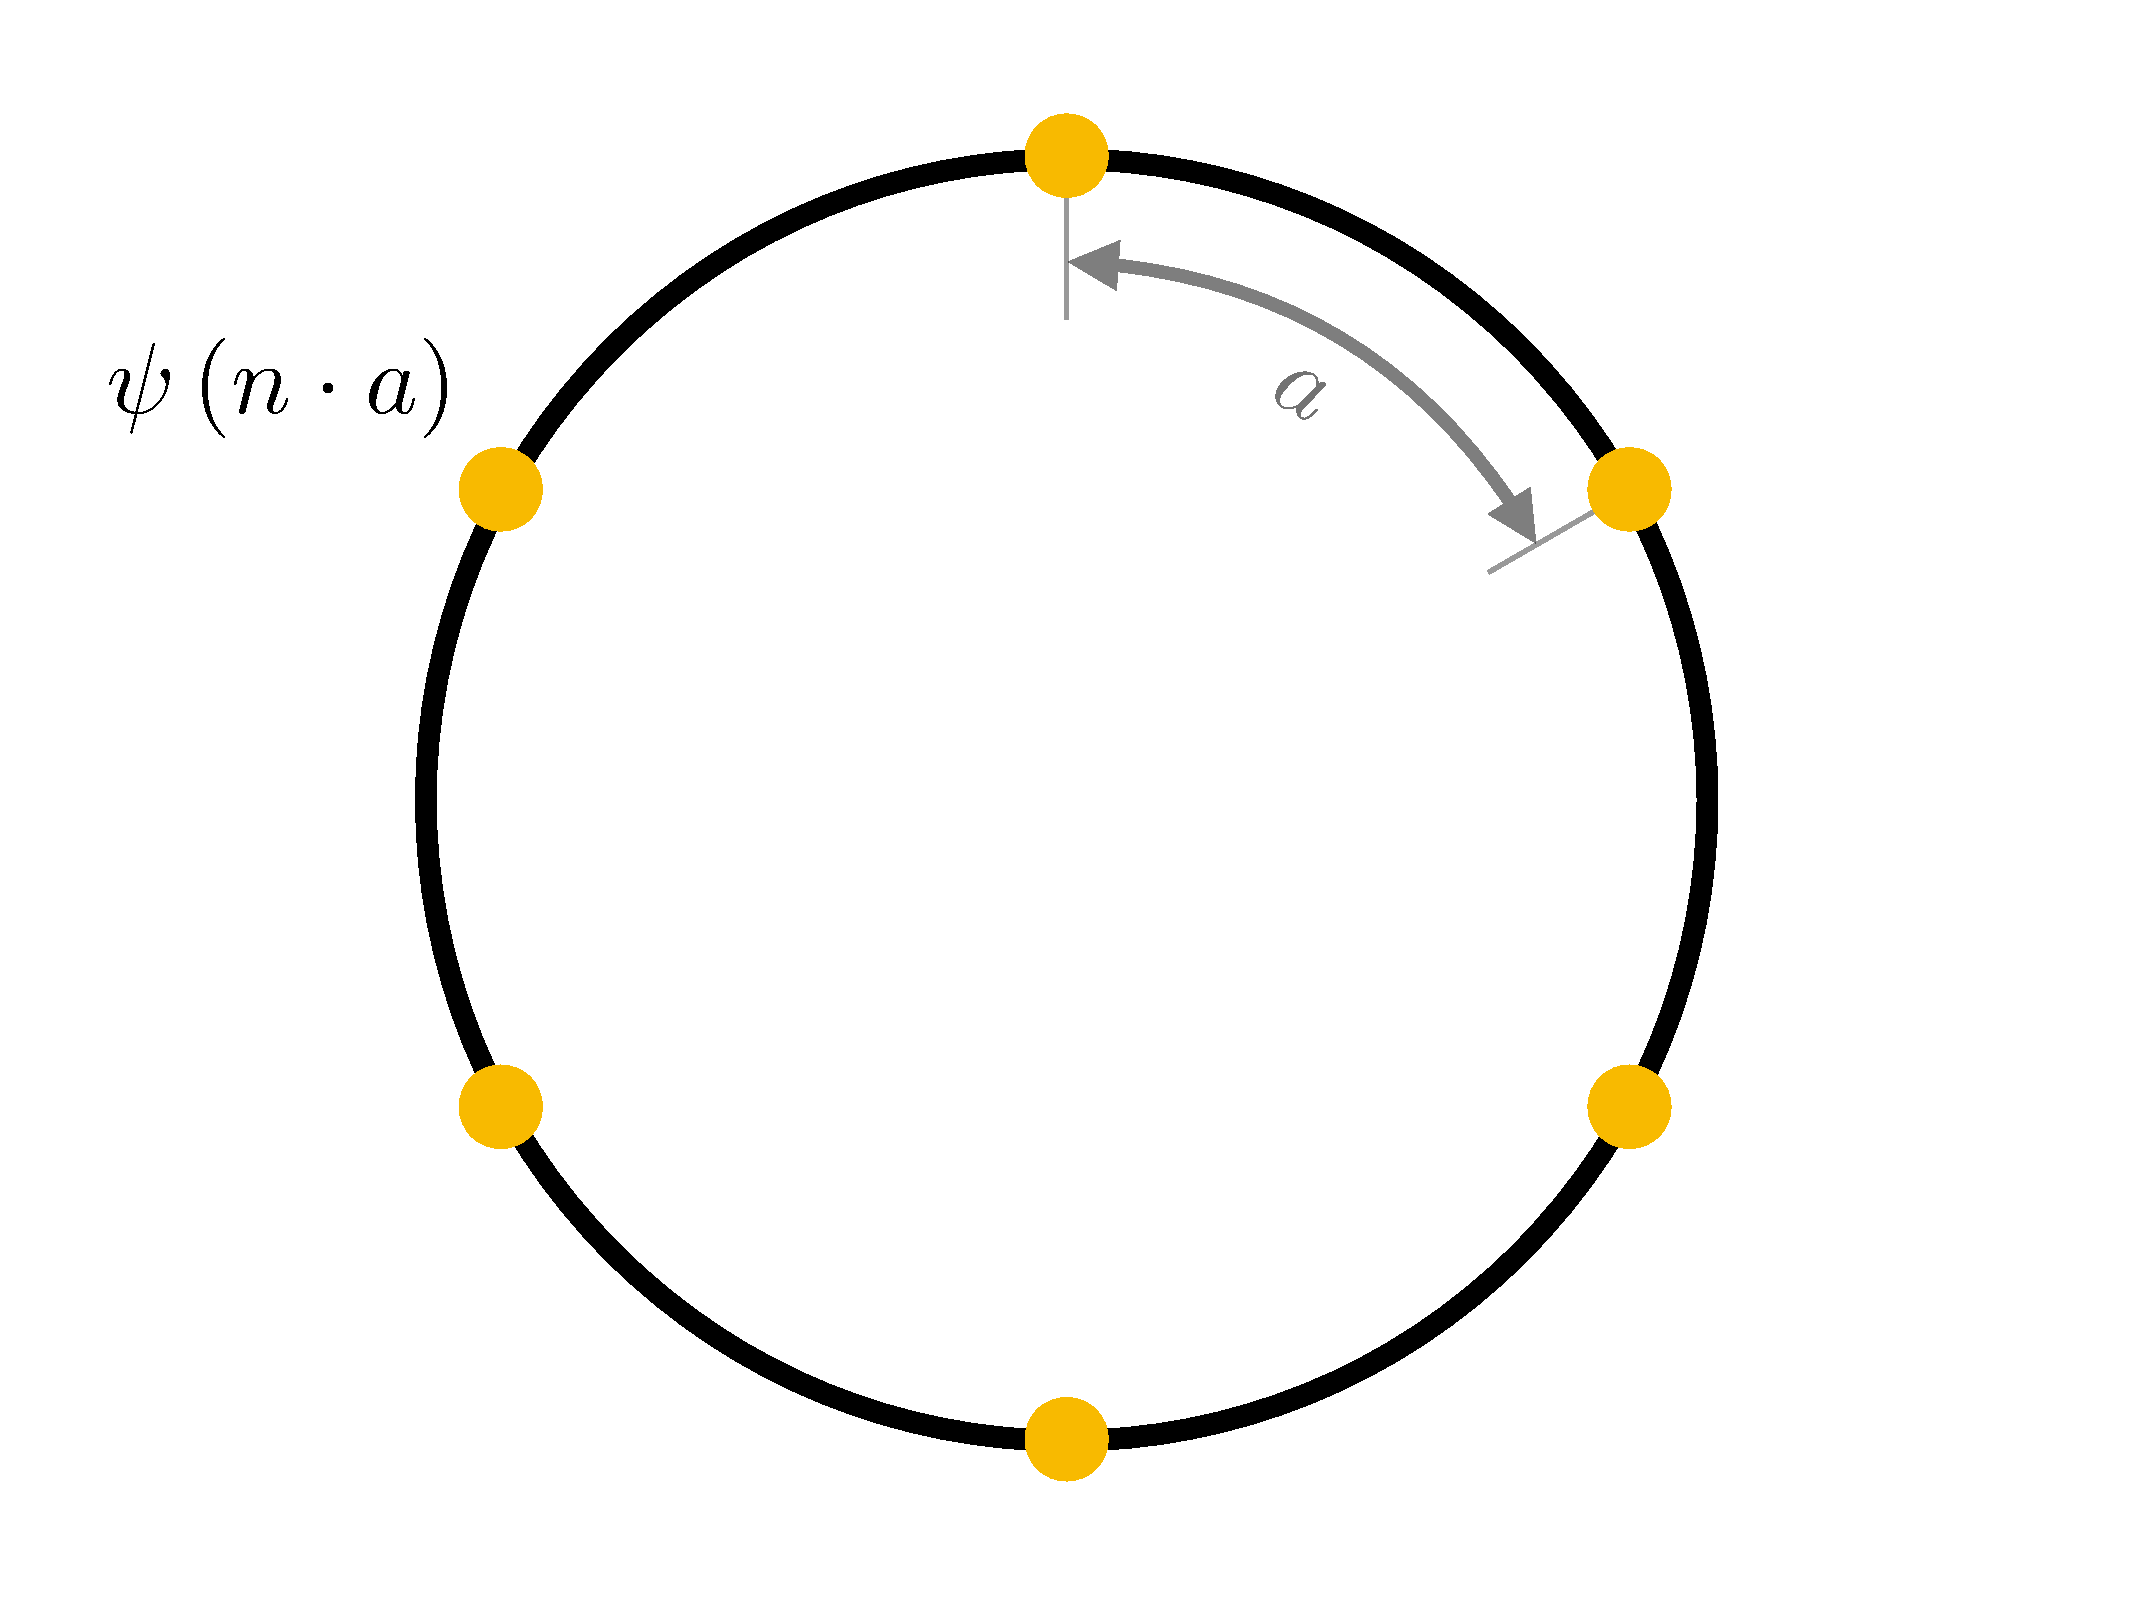
\includegraphics[width=\linewidth]{Figures/NJL1-model-solving/theoretical-fermion-lattice}
		\end{minipage}
	  \hspace{.025\linewidth}
		\begin{minipage}[c]{.45\linewidth}
			\centering
			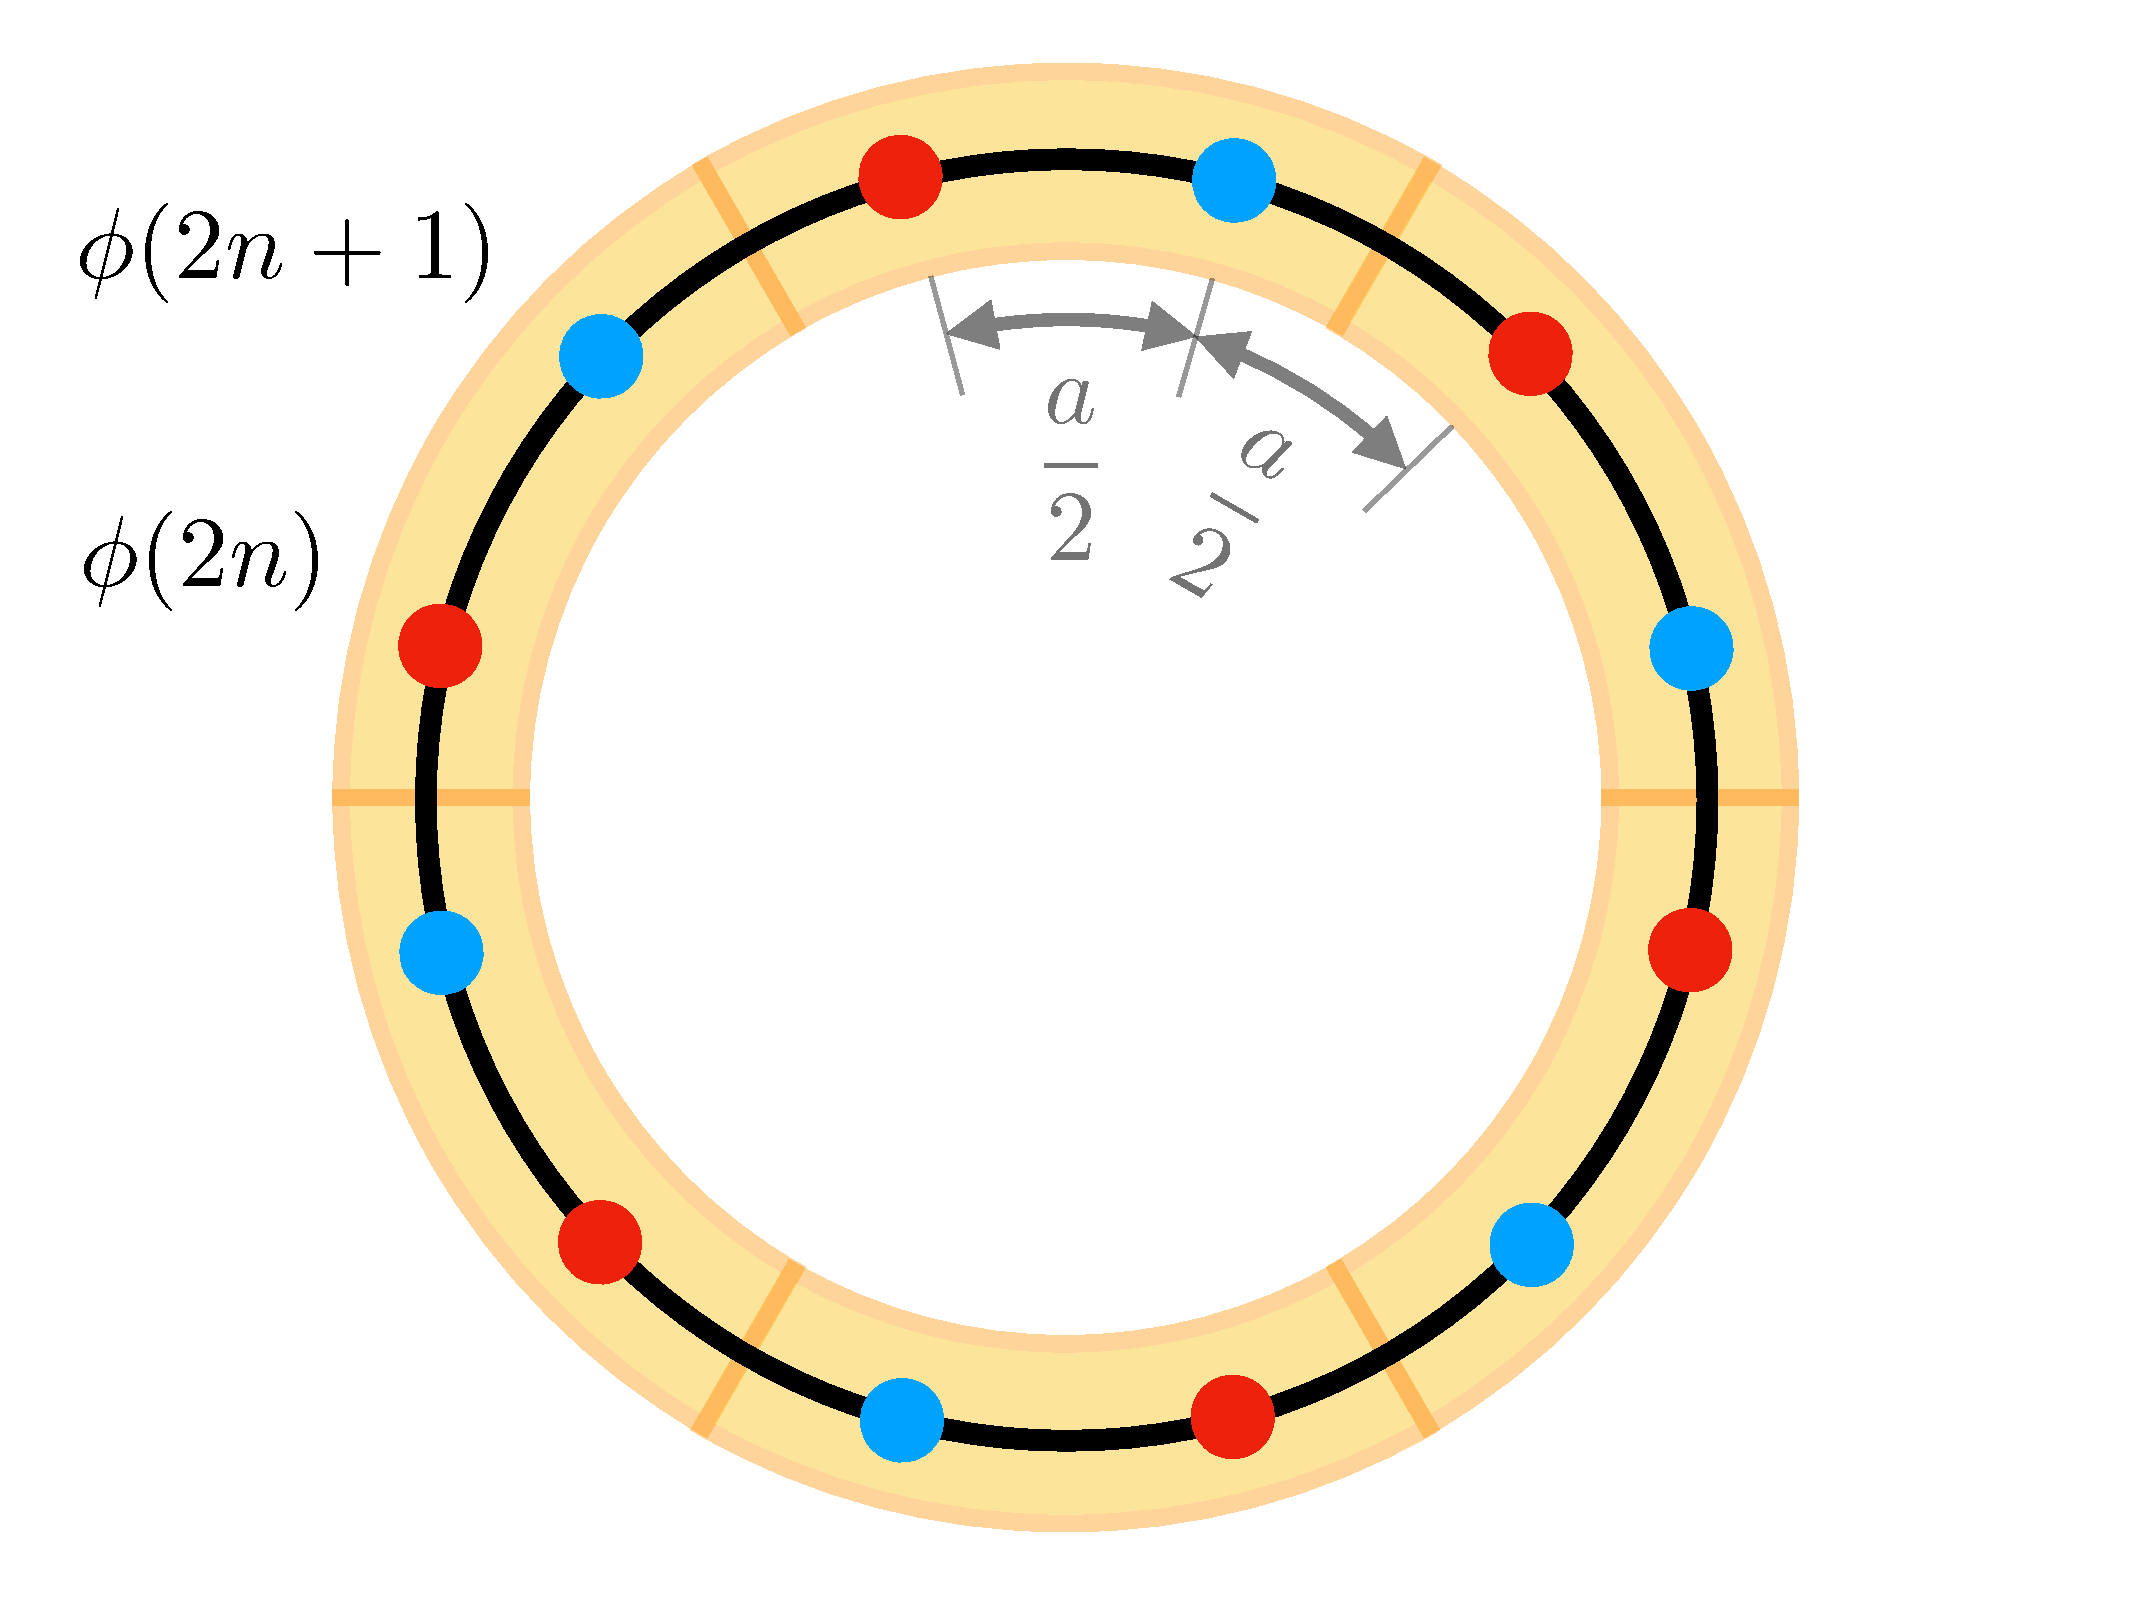
\includegraphics[width=\linewidth]{Figures/NJL1-model-solving/computational-fermion-lattice}
		\end{minipage}
		% \caption{Representations of a fermion lattice in $1+1$ dimensions, with periodic boundary conditions, and for $N=6$ theoretical lattice sites. (Left) Theoretical lattice. (Right) Staggered computational lattice.}
	  % \label{fig:staggered-fermion-lattice}
	\end{figure}

\break

	Sites in the staggered computational lattice are labeled using a parameter $n \in \mathds{Z}$ such that all evaluations of $\psi$ are made at integer multiples of the distance $a$:

	\begin{gather*}
	  \phi(n) \defeq \sqrt{a}
	    \begin{cases}
	      \psi_{+}\qty(\frac{n}{2}a) \qc &2 \mid n \\
	      \psi_{-}\qty(\frac{n-1}{2}a) \qc &2 \nmid n
	    \end{cases}
	\end{gather*}

	These newly defined operators obey the \textbf{canonical commutation relations for fermions}:

	\begin{gather*} \label{eq:fermion-canonical-commutation-relations}
	  \acom{\phi^{\dagger}(p)}{\phi(q)} = \delta_{pq} \qc
	  \acom{\phi(p)}{\phi(q)} = 0
	\end{gather*}

	Finally, thanks to the periodic boundary conditions, we can write:

	\begin{gather*}
	  H_{N}^{(K)} =
	    \frac{i}{a} \sum_{n=0}^{2N-1} \qty[
	    \phi^{\dagger}(n)\phi(n+1) - \phi^{\dagger}(n+1)\phi(n)]
	\end{gather*}

\break

	From this Hamiltonian, we can now recover the \textbf{masless Dirac equation} in the continuum limit; which serves as proof of correctness:

	\begin{gather*}
	  \dot{\phi}(n) = i\com{H_{N}^{(K)}}{\phi(n)} = \frac{\phi(n+1)-\phi(n-1)}{a}
	\end{gather*}

	In terms of the original fields, this is:

	\begin{gather*}
	  \dot{\psi_{+}} = \frac{\Delta \psi_{-}}{\Delta x} \qc
	  \dot{\psi_{-}} = \frac{\Delta \psi_{+}}{\Delta x}
	\end{gather*}

	Lastly, taking the limit when $a \ra 0$:

	\begin{gather*}
	  \pderivative{t}\psi = \hat{\alpha_1}\pderivative{x}\psi \\
	  \hat{\alpha_1} \defeq \gamma_{0}\gamma_{1} = \gamma^{0}\gamma_{1}
	    = -\gamma^{0}\gamma^{1} = \mqty[0 & 1 \\ 1 & 0]
	\end{gather*}

\break

	And it is now straight forward to obtain all other components of the Hamiltonian from the expressions in the Hamiltonian density, which are written in terms of \textbf{Dirac bilinears}.

	\vspace{1em}

	\begin{gather*}
	  H_{N} = H_{N}^{(M)} + H_{N}^{(K)} + H_{N}^{(I)}
	    \label{eq:NJL1-staggered-discretization} \\
	  H_{N}^{(M)} =
	    m \sum_{n=0}^{2N-1} (-1)^{n}\phi^{\dagger}(n)\phi(n) \\
	  H_{N}^{(K)} =
	    \frac{i}{a} \sum_{n=0}^{2N-1} \qty[
	    \phi^{\dagger}(n)\phi(n+1) - \phi^{\dagger}(n+1)\phi(n)] \\
	  H_{N}^{(I)} =
	    - \frac{1}{2a} G_{\pi} \sum_{n=0}^{N-1} \qty[
	      \phi^{\dagger}(2n)\phi(2n) - \phi^{\dagger}(2n+1)\phi(2n+1)
	    ]^{2}
	\end{gather*}

\end{frame}

%% ----------------------------------------------------------------------------

\subsection{Fermion-qubit mapping}

\begin{frame}{Fermion-qubit mapping}

	Generally speaking, quantum computers cannot measure any given operator directly. Therefore, in order to simulate this or any other Hamiltonian in a quantum processor, one needs to efficiently map its component operators onto ones suitable for evaluation in such machines. The most commonly used of these sets are Pauli operators along with the identity: this is what we will use and refer to as the \textbf{Pauli set}.

	\medskip

	It turns out that, in one spatial dimension, spin-$\frac{1}{2}$ particles (i.e. qubits) behave much like fermions. This allows us to implement a mapping between one and the other. The \textbf{Jordan-Wigner transform} associates spin ``down'' and ``up'' with occupied and unoccupied fermion states (or vice versa). Particularly, we will choose:

	\begin{align*}
		\ket{\ua} \equiv \ket{0} &\qc
			\ket{\da} \equiv \ket{1} \\
    \ket{\da} \equiv \phi^{\dagger}\ket{0} &\qc
			\ket{\ua} \equiv \phi\ket{1} \\[5pt]
		\phi \ra \sigma^{+} &\qc \phi^{\dagger} \ra \sigma^{-}
	\end{align*}

\end{frame}

%% ----------------------------------------------------------------------------

\begin{frame}[allowframebreaks]{Jordan-Wigner transform}

	To prove that this is valid, we can define the following equivalences by drawing inspiration from raising and lowering operators in angular momentum theory:

	\begin{align*}
		\sigma^{1} &\equiv \phi^{\dagger} + \phi \\
		\sigma^{2} &\equiv i\qty(\phi^{\dagger} - \phi) \\
		\sigma^{3} &\equiv 1 - 2\phi^{\dagger}\phi
	\end{align*}

	Making use of the properties of fermion creation and annihilation operators, comprised within their canonical commutation relations, these can be shown to behave algebraically like \textbf{Pauli matrices}:

	\begin{align*}
	  \com{\sigma^{p}}{\sigma^{q}} &= 2i\epsilon_{pqr}\sigma^{r} \\
	  \acom{\sigma^{p}}{\sigma^{q}} &= 2\delta_{pq}
	\end{align*}

\break

	We can recover the usual spin raising and lowering hermitian conjugate operators:

	\begin{gather}
	  \sigma^{\pm} \defeq \frac{1}{2}\qty(\sigma^{1} \pm i\sigma^{2})
	\end{gather}

	All this allows us to use these spins as a basic model for fermions:

	\begin{gather} \label{eq:anticommutator-for-single-particle-jordan-wigner}
	  \acom{\phi}{\phi^{\dagger}} = 1 \qra \acom{\sigma^{+}}{\sigma^{-}} = 1
	\end{gather}

	Unfortunately, this only works for single-fermion representations, and needs to be modified once we introduced more than one particle; since independent spins commute, while independent fermions anticommute.

	\begin{gather*}
	  \com{\sigma^{+}(p)}{\sigma^{-}(q)} = \delta_{pq} \qc
	    \acom{\sigma^{+}(p)}{\sigma^{-}(q)} \neq \delta_{pq} \\
	  \com{\phi(p)}{\phi^{\dagger}(q)} \neq \delta_{pq} \qc
	    \acom{\phi(p)}{\phi^{\dagger}(q)} = \delta_{pq}
	\end{gather*}

\break

	A way to fix this issue is by defining $N(l)=\phi^{\dagger}(l)\phi(l)$ as the hermitian number operator for state $l$, and attaching a so called unitary \textbf{string operator} $S(n)$ to the fermion operators:

	\begin{gather*}
		\begin{split}
			S(n)\phi(n) &\ra \sigma^{+}(n) \\
			\phi^{\dagger}(n)S^{\dagger}(n) &\ra \sigma^{-}(n)
		\end{split} \\
		S(n) = \exp[ -i\pi \sum_{l<n} \qty[N(l)+s(l)] ]
	\end{gather*}

	\vspace{-0.5em}

	The $s(l)$ terms in the string operator are scalars associated to \textbf{gauge transformations} and do not add much to the transform. With this new mapping, Pauli matrices get redefined to:

	\begin{align*}
		\sigma^{1}(n) &\equiv
			\phi^{\dagger}(n)S^{\dagger}(n) + S(n)\phi(n) \\
		\sigma^{2}(n) &\equiv
			i\qty[\phi^{\dagger}(n)S^{\dagger}(n) - S(n)\phi(n)] \\
		\sigma^{3}(n) &\equiv
			1 - 2\phi^{\dagger}(n)\phi(n)
	\end{align*}

\break

	We now retrieve the correct statistics. Of course, we would like to express the string operator in terms of the Pauli set so that we can move it to the other side of the transformation. Fortunately, we can do so by expanding the number operators:

	\begin{gather*}
	  \exp[\pm i\pi \sum_{l<n} N(l)] =
		  \prod_{l<n}\exp[\pm i\pi \phi^{\dagger}(l)\phi(l)] =
		  \prod_{l<n}\qty[1-2\phi^{\dagger}(l)\phi(l)] =
		  \prod_{l<n}\sigma^3(l) \\
		S(n) = \prod_{l<n} e^{-i\pi s(l)} \sigma^3(l)
	\end{gather*}

	Finally, our \textbf{choice of gauge} will be such that $s(l) = s \in (-1,1]$ $\forall l$ and the string operator is hermitian for all values of $n$. All in all, this can be achieved by making $s=0$, which gives:

	\begin{gather*}
		\phi(n) \ra \qty[\prod_{l<n} \sigma^3(l)]\sigma^{+}(n) \qc
		\phi^{\dagger}(n) \ra \qty[\prod_{l<n} \sigma^3(l)]\sigma^{-}(n)
	\end{gather*}

\end{frame}

%% ----------------------------------------------------------------------------

\begin{frame}[allowframebreaks]{Refactoring the NJL Hamiltonian}

	Now that we have a way of converting from fermion to spin operators, we can apply it to the NJL Hamiltonian:

	\begin{align*}
	  H_{N}^{(M)} &\qra
	    \frac{m}{2} \sum_{n=0}^{2N-1} (-1)^{n+1}\sigma^{3}(n) \\
	  H_{N}^{(K)} &\qra
	    \frac{i}{a} \sum_{n=0}^{2N-1}
	    \qty[\sigma^{-}(n)\sigma^{+}(n+1) - \sigma^{-}(n+1)\sigma^{+}(n)] \\
	  H_{N}^{(I)} &\qra
	    \frac{G_{\pi}}{4a} \sum_{n=0}^{N-1} \qty[\sigma^{3}(2n)\sigma^{3}(2n+1) - N]
	\end{align*}

	We will only be interested in studying the \textbf{Chiral limit} (i.e. $m=0$), which justifies dropping the entire mass term. From the interaction Hamiltonian we will get an adiabatic modification term of the form $\frac{G_{\pi}N}{4a}$; this will also be dropped for the moment.

\break

	Hence, with periodic boundary conditions $\sigma^{p}(N)=\sigma^{p}(0)$ and expressed in quantum computing notation $\qty(\mathds{1}_{n},X_{n},Y_{n},Z_{n}) \equiv \sigma^{p}(n)$ for $p=\qty(0,1,2,3)$, our refactored Hamiltonian $P_{N} \defeq 2aH_{N}$ will adopt the form:

	\begin{gather} \label{eq:NJL1-refactored-hamiltonian}
	  P_{N} =
	    \sum_{n=0}^{2N-1} \qty[X_{n+1} Y_{n} - Y_{n+1} X_{n}] +
	      \frac{G_{\pi}}{2} \sum_{n=0}^{N-1} Z_{2n+1} Z_{2n}
	\end{gather}

	One important feature of this operator is that its size (i.e. number of terms) \textbf{grows polynomially} with the size of the system $N$. It is also interesting to notice that this operator can be expressed in a recursive layout:

	\begin{align*}
		P_{N+1} =& P_{N}
				- Y_{2N-1} X_{0} + X_{2N-1} Y_{0} + Y_{2N+1} X_{0} - X_{2N+1} Y_{0} \\
			&+ X_{2N} Y_{2N-1} - Y_{2N} X_{2N-1} + X_{2N+1} Y_{2N} - Y_{2N+1} X_{2N}
				+ \frac{G_{\pi}}{2} \qty(Z_{2N+1} Z_{2N})
	\end{align*}

\end{frame}


%% ----------------------------------------------------------------------------

\subsection{Space parametrization and state preparation}

\begin{frame}{Space parametrization and state preparation}

	Once we have ways of measuring our Hamiltonian, we need to be able to explore different quantum states; a process known as \textbf{state preparation}. This can be achieved by parametrizing the Hilbert/Fock space of states representing the system, and finding a way to prepare the corresponding quantum state in the processor given any combination of those parameters.

	\begin{multicols}{2}

		For this task we will be employing some of the IBM-Q quantum computers and simulators; accessible through the cloud via the \texttt{Qiskit} framework. Nevertheless, there is one major shortcoming: the dimension of the space at hand grows exponentially with the number of qubits $2N$ used in the representation of the system. This means that the parametrization will become too large to handle both in state of the art and forthcoming machines unless it is treated in a smart way.

		\columnbreak

		\begin{center}
			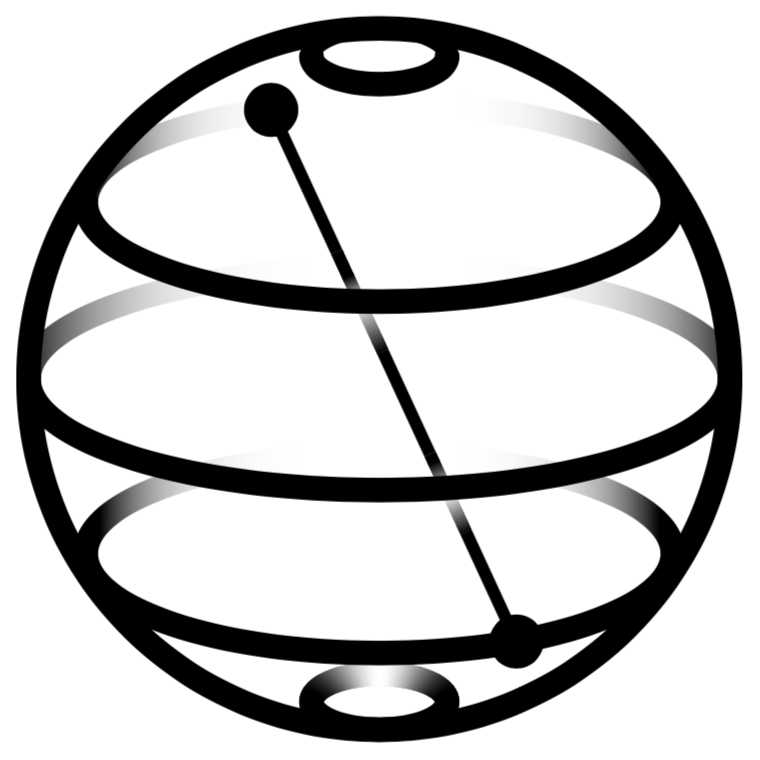
\includegraphics[width=.2\paperwidth]{Figures/qiskit}
		\end{center}
		\begin{center}
			
\includegraphics[width=.1\paperwidth]{Figures/ibm}
		\end{center}

	\end{multicols}

\end{frame}

%% ----------------------------------------------------------------------------

\begin{frame}[allowframebreaks]{Custom symmetry-based parametrization ansatz}

	While general, it is easy to notice that the implementation of any variant of the unitary coupled cluster ansatz is still cumbersome and can depend on a large number of parameters based on the chosen order of truncation. We will now introduce a new ansatz inspired by the shape of our refactored Hamiltonian. For this task, we will analyze the two distinct parts in our Hamiltonian independently; since these will dominate in two \textbf{different regimes}:

	\begin{multicols}{2}

		\begin{center}
			\underline{\textbf{INFINITELY STRONG INTERACTIONS}}\\
			\small{\emph{Interaction term dominates (i.e. $G_{\pi} \ra \infty$)}}
			\begin{gather*}
				G_{N} \defeq \sum_{n=0}^{N-1} Z_{2n+1}Z_{2n}
			\end{gather*}
		\end{center}

		\columnbreak

		\begin{center}
			\underline{\textbf{INFINITELY WEAK INTERACTIONS}}\\
			\small{\emph{Kinetic term dominates (i.e. $G_{\pi} \ra 0$)}}
			\begin{gather*}
			  K_{N} \defeq \sum_{n=0}^{2N-1} \qty[ X_{n+1}Y_{n} - Y_{n+1}X_{n} ]
			\end{gather*}
		\end{center}

	\end{multicols}

	Let us call each computational basis state by the decimal translation of its binary form:

	\begin{gather*}
	  \ket{0} \defeq \ket{\bin\dots0000} \qc
	  \ket{1} \defeq \ket{\bin\dots0001} \qc
	  \ket{2} \defeq \ket{\bin\dots0010} \qc
	  \cdots
	\end{gather*}

\break

	For the \textbf{interaction term} we notice that:

	\medskip

	\begin{itemize}
	  \item We can cycle in steps of two computational lattice sites.
	  \item We can change the position of any theoretical lattice site; since the interaction only occurs between positive and negative energy components at the same spot.
	  \item We can interchange positive and negative components in any number of theoretical lattice sites. We call each of these a \emph{swap transformation}.
	  \item We can flip every component $0 \lra 1$ in any number of theoretical lattice sites. We call each of these a \emph{flip transformation}.
	\end{itemize}

	\medskip

	This means that for $N=2$ (i.e. $2^{2N}=16$ basis states):

	\begin{gather*}
	  \ket{0} \equiv \ket{3} \equiv \ket{12} \equiv \ket{15} \\
	  \ket{1} \equiv \ket{2} \equiv \ket{4} \equiv \ket{7} \equiv
	    \ket{8} \equiv \ket{11} \equiv \ket{13} \equiv \ket{14} \\
	  \ket{5} \equiv \ket{6} \equiv \ket{9} \equiv \ket{10}
	\end{gather*}

\break

	Which represent the partition in degenerate subspaces of associated eigenvalues $\qty{+2,0,-2}$ respectively. These eigenvalues come from each theoretical lattice site in the spin-Z basis contributing with either $\pm 1$. Notice that the eigenvalues of this operator are always symmetrically disposed about zero, which means that $\forall N$:

	\begin{gather*}
	  \gamma_{\text{max}}^{N} = - \gamma_{\text{min}}^{N}
	\end{gather*}

	The interaction is maximum inside any theoretical lattice site whenever there is equal presence of both positive and negative energy components; conversely, the interaction is minimum whenever there is only one component present. Of course, the maximum (minimum) of the operator occurs when all theoretical lattice sites are maximized (minimized) individually:

	\begin{gather*}
	  \ket{\gamma_{\text{max}}}_{n} \in \{\ket{\bin00}, \ket{\bin11}\} \qc
	  \ket{\gamma_{\text{min}}}_{n} \in \{\ket{\bin01}, \ket{\bin10}\} \\[5pt]
	  \ket{\gamma_{\text{max}}^{N}} \equiv
	    \ket{\gamma_{\text{max}}}^{\otimes N} \qc
	  \ket{\gamma_{\text{min}}^{N}} \equiv
	    \ket{\gamma_{\text{min}}}^{\otimes N}
	\end{gather*}

\break

	Moving on to the \textbf{kinetic term} we have:

	\medskip

	\begin{itemize}
	  \item We can cycle in steps of one computational lattice site. We call this a \emph{cycling transformation}.
	  \item We cannot change the position of any theoretical lattice site; since the computational lattice sites now form a chain with their nearest neighbors.
	  \item If we interchange positive and negative components in all theoretical lattice sites, the resulting expectation value flips its sign (i.e. \emph{global swap transformations} are antisymmetric).
	  \item Flip transformations do not represent any apparent symmetry.
	\end{itemize}

	\medskip

	Once more, this operator has its eigenstates symmetrically disposed around zero. Also, global swap transformations are equivalent to complex conjugation:

	\begin{gather*}
		\kappa_{\text{max}}^{N} = -\kappa_{\text{min}}^{N} \\
		K_{N}^{\dagger} = \qty(K_{N}^{*})^{T} = \qty(-K_{N})^{T} = K_{N} \qRa
	    K_{N}^{T} = -K_{N} = K_{N}^{*}
	\end{gather*}

\break

	\begin{table}[!bp]
	  \centering
	  \caption{Global swap transformations for the $N=2$ basis states according to their number of particles.}
	  \label{tab:symmetry-ansatz-basis2-swaps}
	  \begin{tabular}{ c l }
	    \hline
	    % \rule{0pt}{14pt}
	    $N_\text{particles}$ & Global swap transformations \\
	    \hline
	    \hline
	    % \rule{0pt}{14pt}
	    $0$ & $\ket{0} \lra \ket{0}$ \\
	    \hline
	    $1$ & $\ket{1} \lra \ket{2} \qc \ket{4} \lra \ket{8}$ \\
	    \hline
	    $2$ & $\ket{3} \lra \ket{3} \qc \ket{5} \lra \ket{10} \qc
	      \ket{6} \lra \ket{9} \qc \ket{12} \lra \ket{12}$ \\
	    \hline
	    $3$ & $\ket{7} \lra \ket{11} \qc \ket{13} \lra \ket{14}$ \\
	    \hline
	    $4$ & $\ket{15} \lra \ket{15}$ \\
	    \hline
	  \end{tabular}
	\end{table}

	\begin{table}[!bp]
	  \centering
	  \caption{Cycles for the $N=2$ basis states according to their number of particles.}
	  \label{tab:symmetry-ansatz-basis2-cycles}
	  \begin{tabular}{ c l }
	    \hline
	    % \rule{0pt}{14pt}
	    $N_\text{particles}$ & Cycles \\
	    \hline
	    \hline
	    % \rule{0pt}{14pt}
	    $0$ & $\ket{0}$ \\
	    \hline
	    $1$ & $\ket{1} \lra \ket{2} \lra \ket{4} \lra \ket{8}$ \\
	    \hline
	    $2$ & $\ket{3} \lra \ket{6} \lra \ket{12} \lra \ket{9} \qc
	      \ket{5} \lra \ket{10}$ \\
	    \hline
	    $3$ & $\ket{7} \lra \ket{14} \lra \ket{13} \lra \ket{11}$ \\
	    \hline
	    $4$ & $\ket{15}$ \\
	    \hline
	  \end{tabular}
	\end{table}

\break

	If an eigenstate is not degenerate, it must comply with the rule that all amplitudes multiplying the states that make up its superposition, and which are related by a cycling transformation, must be the same up to a constant \emph{phase factor}:

	\begin{gather*}
	  e^{i\phi} \in
	    \qty{ \exp(i \frac{2\pi}{p} n) \qq{:} n \in \mathds{Z} \qq{and}
	    p \defeq \text{size of the smaller cycle} }
	\end{gather*}

	Finally, because this operator is made out of the Pauli X and Y matrices, and these matrices ---regardless of any phase factors--- flip the state they are applied to (i.e. $0 \lra 1$), we can see that any maximum (minimum) eigenstate will necessarily have the \textbf{same number of occupied and unoccupied states}. If we naively parametrize the space of states with this number of particles, we will get a prohibitive parametrization that grows exponentially in the number of basis states as $\binom{2N}{N}$. However, if we assume that these eigenstates are not degenerate, we can apply the above mentioned rules to build a simpler general form for them.

\break

	Because the smallest cycle for $N=2$ is of size two, any phase factors between elements of the same cycle can only be $\pm 1$. Also, we need to make sure that a swap transformation in all theoretical lattice sites ---equivalent to complex conjugation--- applied to the either the maximum or minimum eigenstate, reproduces its counterpart.

	\begin{gather*}
	  \alpha \frac{1}{\sqrt{2}} \qty(\ket{3}+\ket{12}) -
	  \beta \frac{1}{\sqrt{2}} \qty(\ket{6}+\ket{9})  +
	  \delta \frac{i}{\sqrt{2}} \qty(\ket{5} - \ket{10})
	\end{gather*}

	Which can then be converted into a general normalized form by resorting to an analogy with spherical coordinates. This results in the \textbf{symmetry based parametrization} (SBP):

	\begin{gather*}
	  \ket{\text{SBP}_{2} \qty(\theta, \eta)} \defeq
	    \sin(\theta)\sin(\eta) \ket{\gamma_{\text{max}}^2} -
	    \sin(\theta)\cos(\eta) \ket{\gamma_{\text{min},1}^2} + i
	    \cos(\theta) \ket{\gamma_{\text{min},2}^2} \\[5pt]
	  \ket{\gamma_{\text{max}}^2} \defeq
	    \frac{\ket{3}+\ket{12}}{\sqrt{2}} \qc
	  \ket{\gamma_{\text{min},1}^2} \defeq
	    \frac{\ket{6}+\ket{9}}{\sqrt{2}} \qc
	  \ket{\gamma_{\text{min},2}^2} \defeq
	    \frac{\ket{5} - \ket{10}}{\sqrt{2}}
	\end{gather*}

\break

	As a matter of fact, this state can indeed evaluate to the minimum and maximum eigenstates of the operator when $N=2$:

	\begin{gather*}
	  \ket{\kappa_{\text{max}}^{2}} =
	    \frac{1}{2\sqrt{2}} \qty(\ket{3}-\ket{6}-\ket{9}+\ket{12}) -
	    \frac{i}{2} \qty(\ket{5}-\ket{10}) \\
	  \ket{\kappa_{\text{min}}^{2}} =
	  \frac{1}{2\sqrt{2}} \qty(\ket{3}-\ket{6}-\ket{9}+\ket{12}) +
	  \frac{i}{2} \qty(\ket{5}-\ket{10})
	\end{gather*}

	The particular choice when assigning the basis states in the spherical coordinates analogy, was made so that these maximum and minimum eigenstates evaluate for simple values of the parameters:

	\begin{gather*}
	  \ket{\kappa_{\text{max}}^{2}} \equiv
	    \ket{\text{SBP}_{2} \qty(\frac{3\pi}{4}, \frac{\pi}{4})} \qc
	  \ket{\kappa_{\text{min}}^{2}} \equiv
	    \ket{\text{SBP}_{2} \qty(\frac{\pi}{4}, \frac{\pi}{4})} \\
	  \ket{\gamma_{\text{max}}^{2}} \equiv
	    \ket{\text{SBP}_{2} \qty(\frac{\pi}{2}, \frac{\pi}{2})} \qc
	  \ket{\gamma_{\text{min},1}^{2}} \equiv
	    \ket{\text{SBP}_{2} \qty(\frac{\pi}{2}, 0)} \qc
	  \ket{\gamma_{\text{min},2}^{2}} \equiv
	    \ket{\text{SBP}_{2} \qty(0, 0)}
	\end{gather*}

\end{frame}

%% ----------------------------------------------------------------------------

\begin{frame}[allowframebreaks]{Parametrization ansatz implementation}

	In order to implement this parametrization on any of the IBM-Q quantum computers, we need to be able to write it down as a quantum circuit. This means that it has to expressed through an unitary operator $U\qty(\theta, \eta)$ in the form:

	\begin{gather}
	  \ket{\text{SBP}_{2} \qty(\theta, \eta)} =
	    U\qty(\theta, \eta) \ket{\text{SR}}
	\end{gather}

	At first we will only be interested in obtaining the ground state energy of our system for positive values of the coupling constant (i.e. we will only need the minimum eigenstates), this allows us to simplify even further the parametrization introduced in the previous section. This will allow us to reduce the subspace we are looking into from three dimensions down to two.

	\begin{gather}
	  \ket{\gamma} \equiv
	    \ket{\gamma_{\text{min},2}^2} \defeq
	    \frac{\ket{5} - \ket{10}}{\sqrt{2}} \equiv
	    \ket{\text{SBP}_{2} \qty(0, \frac{\pi}{4})} \\
	  \ket{\kappa} \defeq
	    \frac{\ket{3}-\ket{6}-\ket{9}+\ket{12}}{2} \equiv
	    \ket{\text{SBP}_{2} \qty(\frac{\pi}{2}, \frac{\pi}{4})}
	\end{gather}

\break

	\begin{multicols}{2}

		This will effectively cut down the degrees of freedom from two to just one (i.e. fixing $\eta=\pi/4$). However, having now only two distinguishable quantum states, we can choose to ease the parametrization to account for the entirety of the Hilbert space associated to the \textbf{qubit} they comprise; spuriously increasing the degrees of freedom back to two, but making the implementation as a quantum circuit conceptually easier.

		\medskip

		We will parametrize an \textbf{ancilla qubit}, and then map its basis states to the two basis states of the subspace that we are interested in exploring.

		\columnbreak

		\begin{center}
			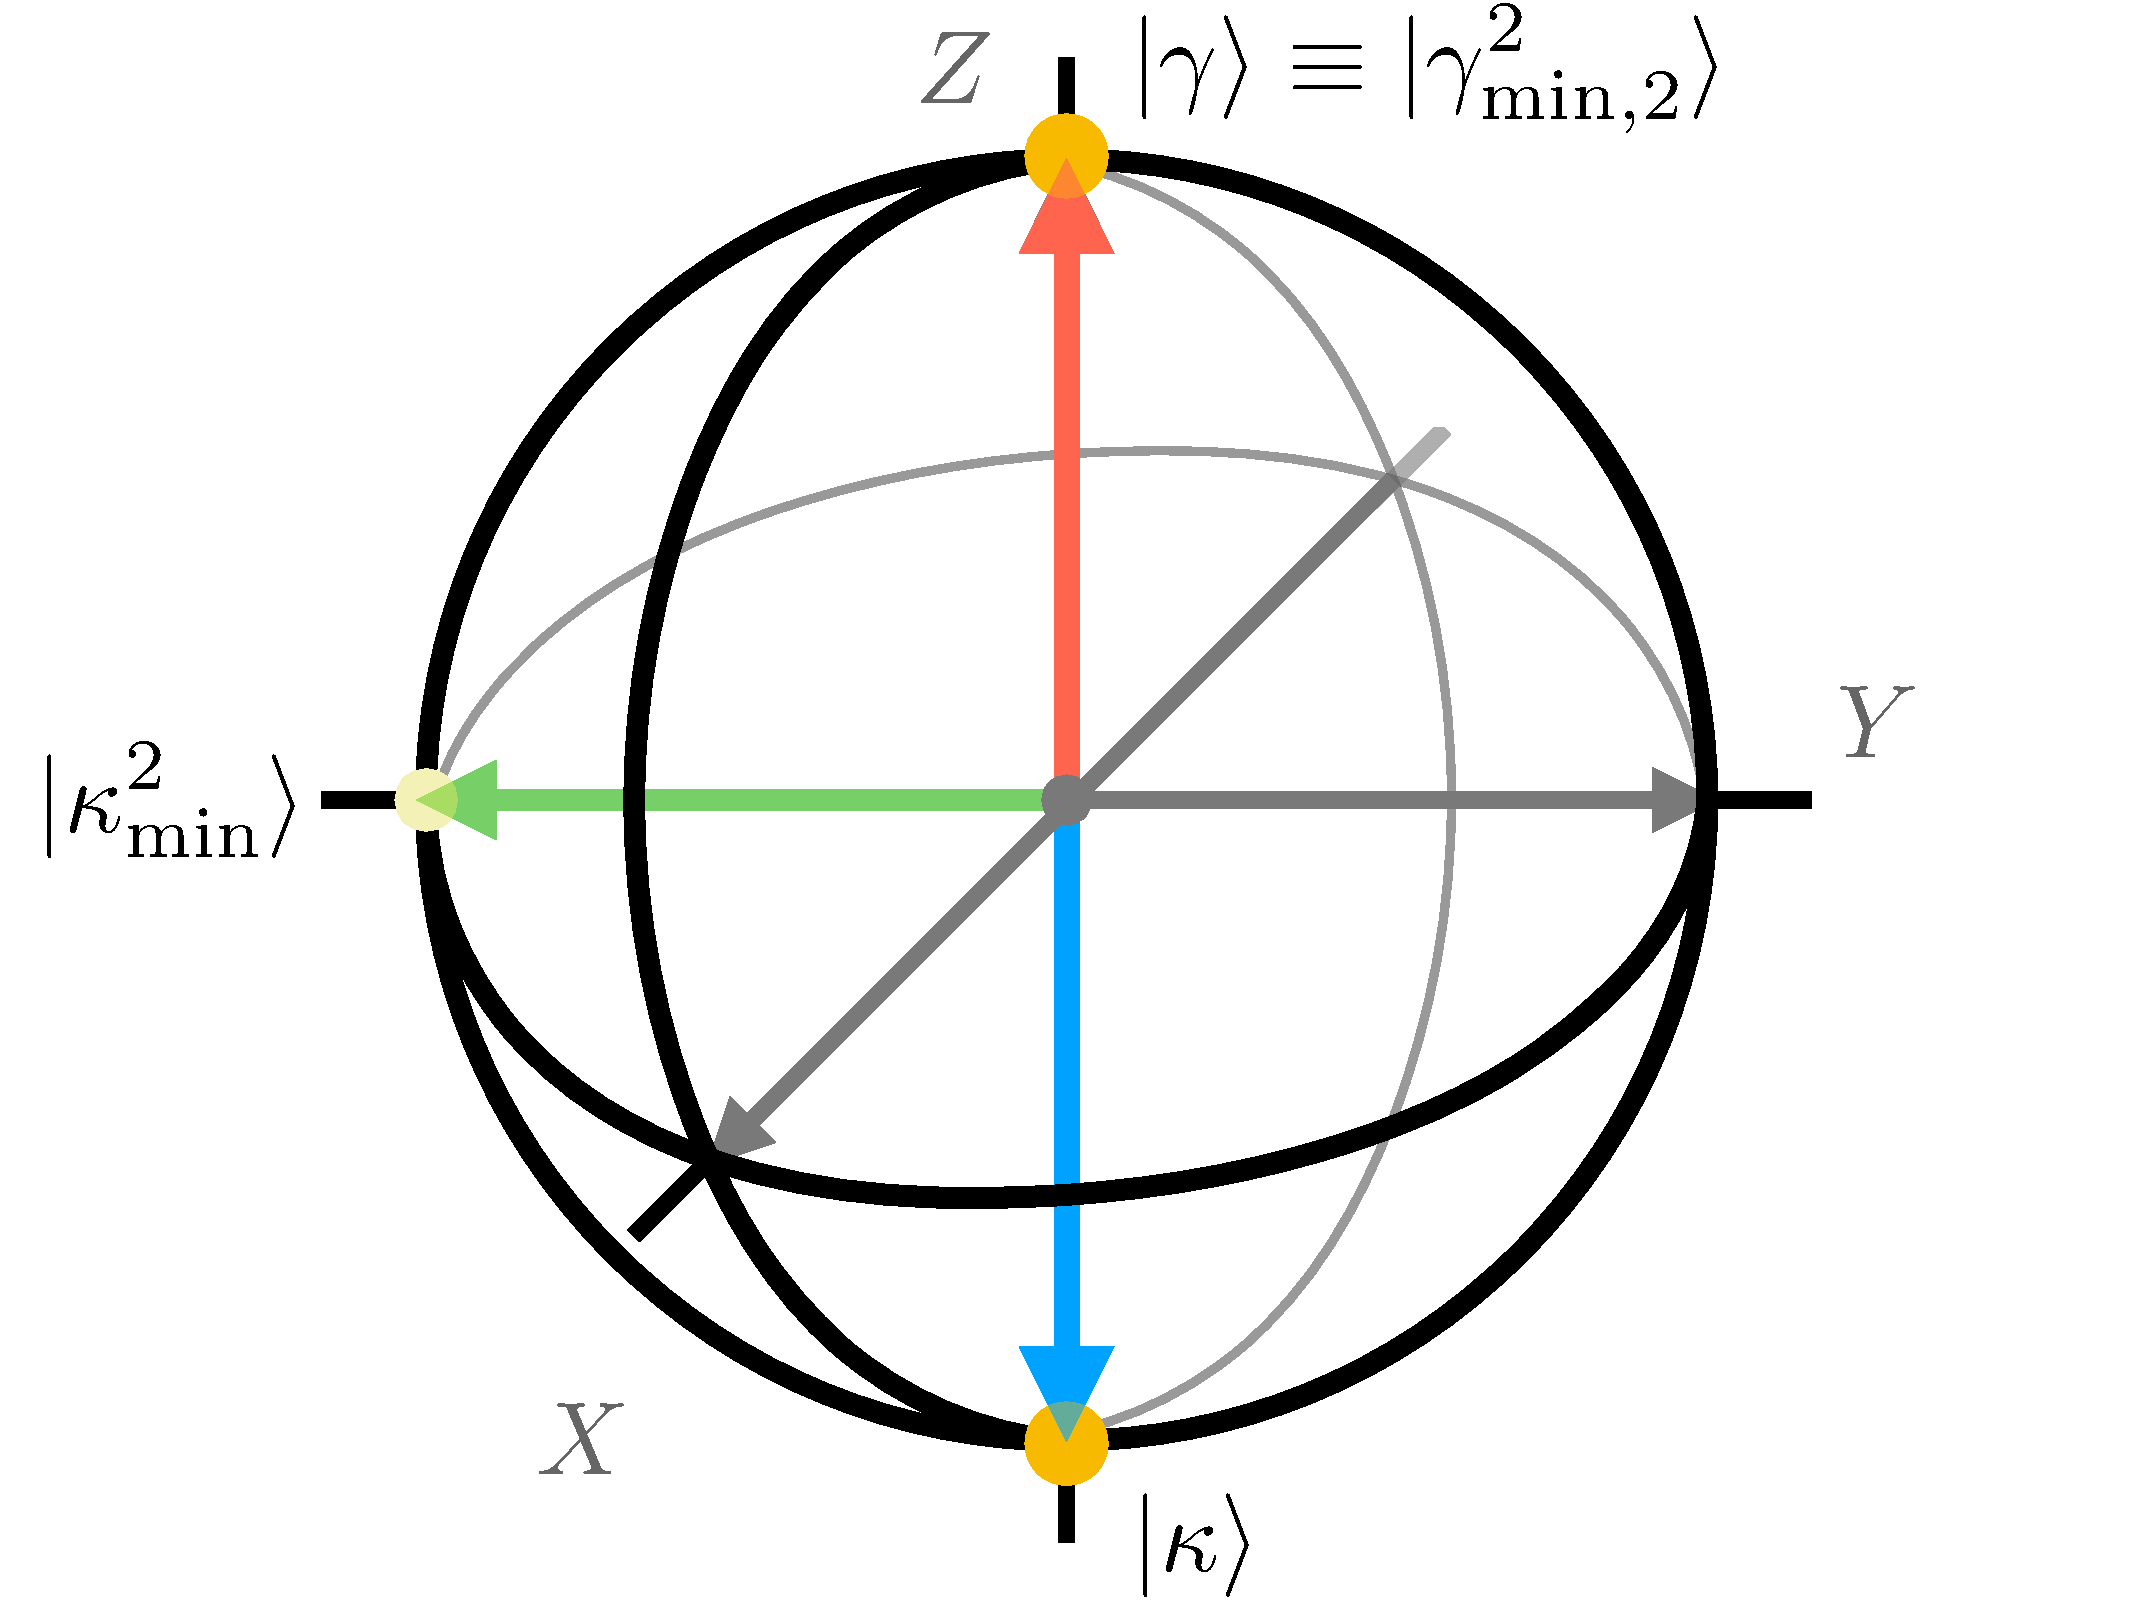
\includegraphics[width=.4\paperwidth]{Figures/NJL1-model-solving/bloch-sphere}
		\end{center}

	\end{multicols}

\break

	\begin{figure}[!p]
		\centering
		\begin{minipage}[c]{.45\linewidth}
			\centering
			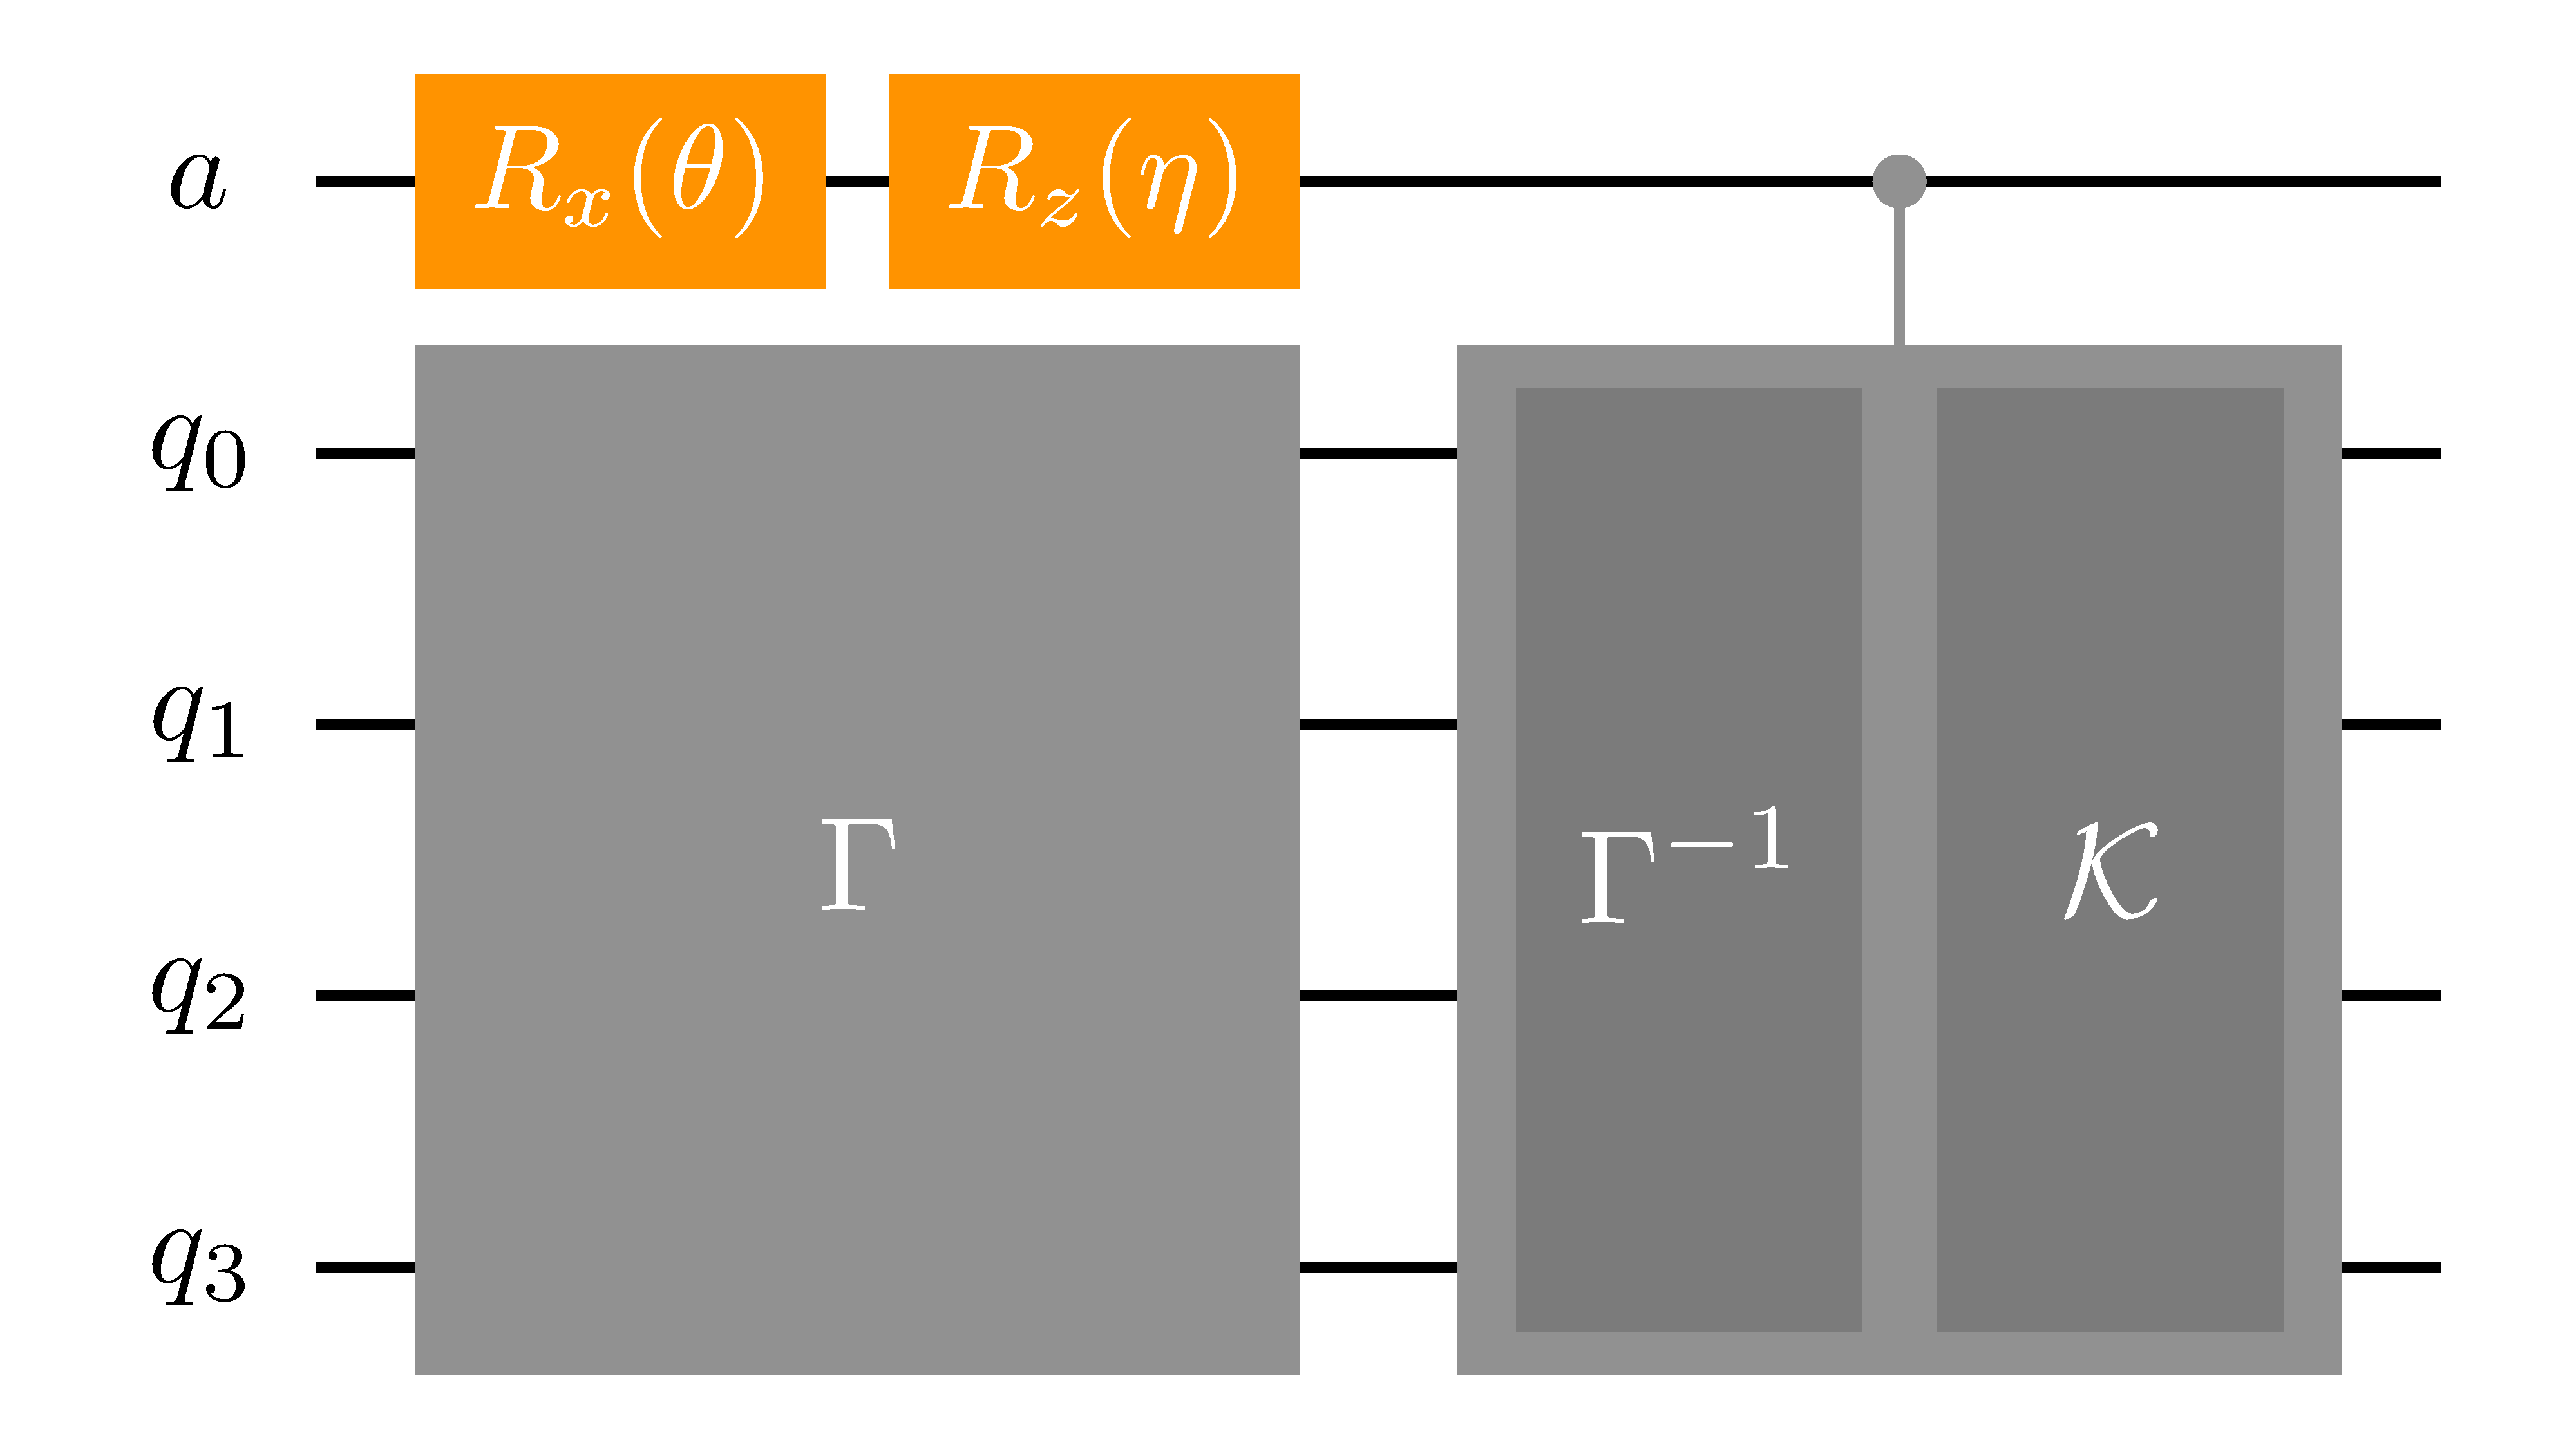
\includegraphics[width=\linewidth]{Figures/NJL1-model-solving/ansatz-implementation-ancilla-mapping}
		\end{minipage}
		\hspace{.025\linewidth}
		\begin{minipage}[c]{.45\linewidth}
			\centering
			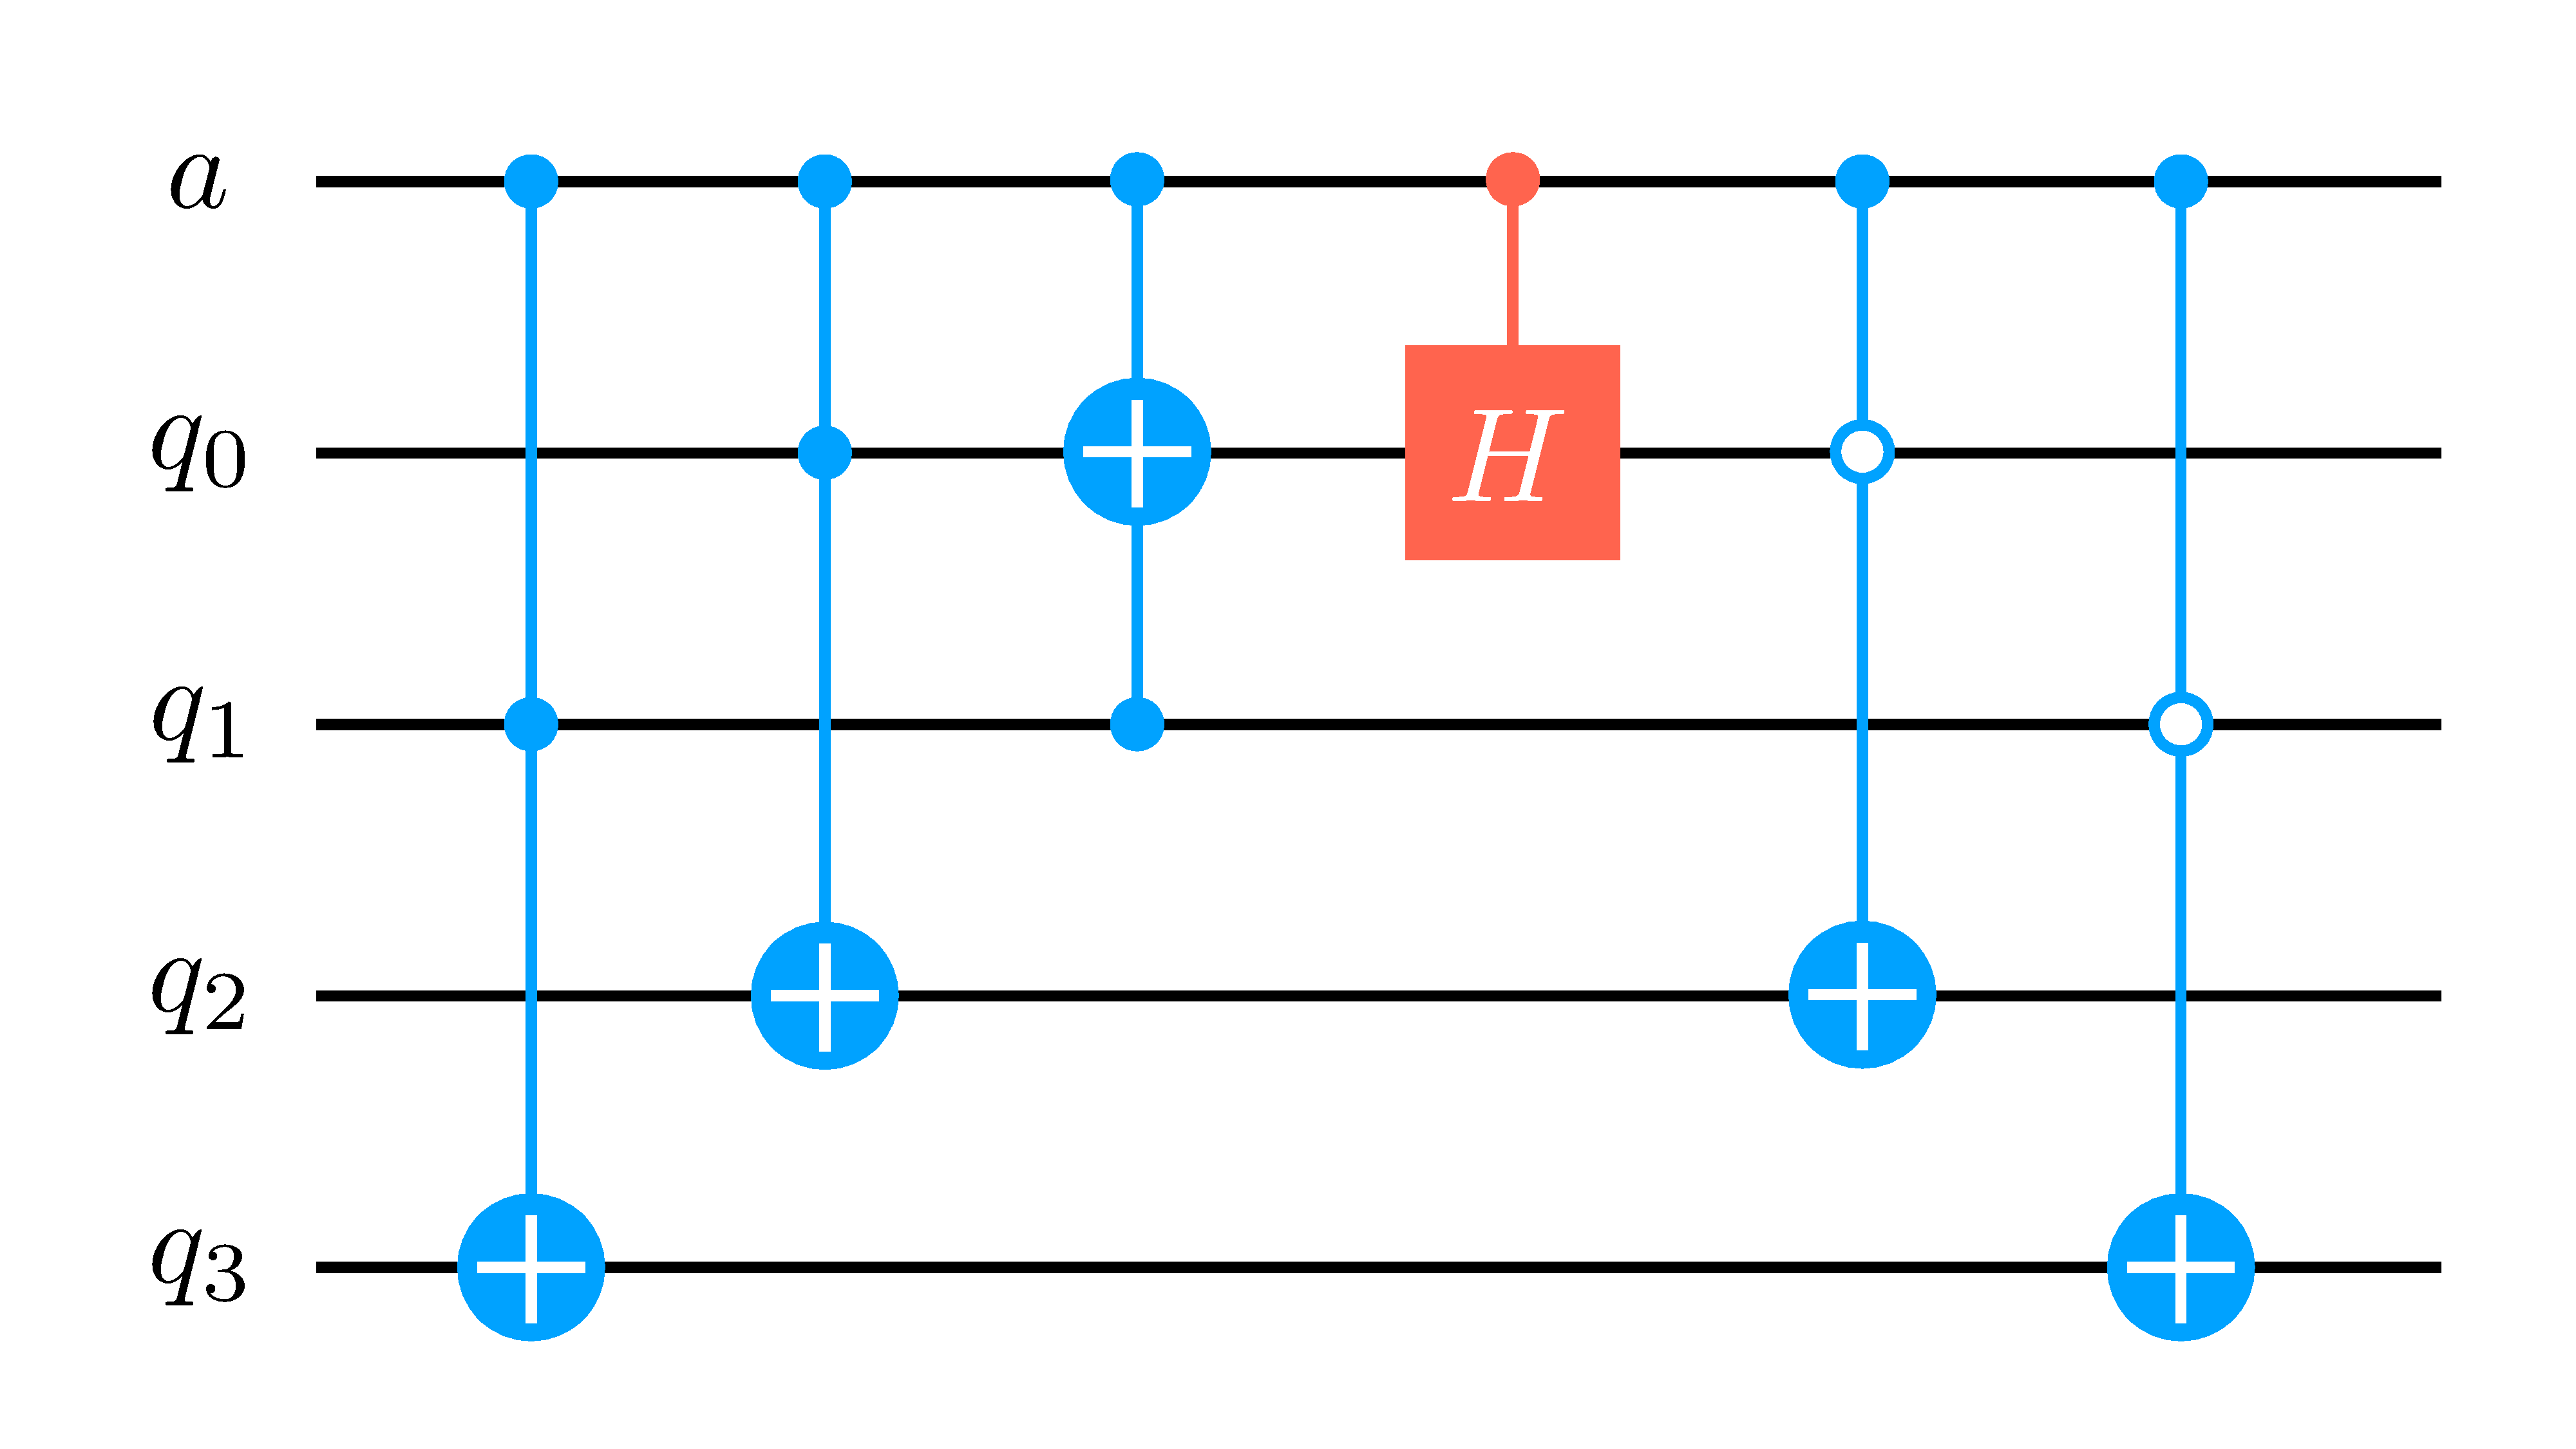
\includegraphics[width=\linewidth]{Figures/NJL1-model-solving/ansatz-implementation-controlled-gammakappa}
		\end{minipage}
		\caption{(Left) Quantum circuit to map the ancilla qubit onto the target qubit Hilbert space in our system. (Right) Simplified controlled $\mathcal{K}\Gamma^{-1}$ gate.}
	\end{figure}

\break

	\begin{figure}[!p]
		\centering
		\begin{minipage}[c]{.45\linewidth}
			\centering
			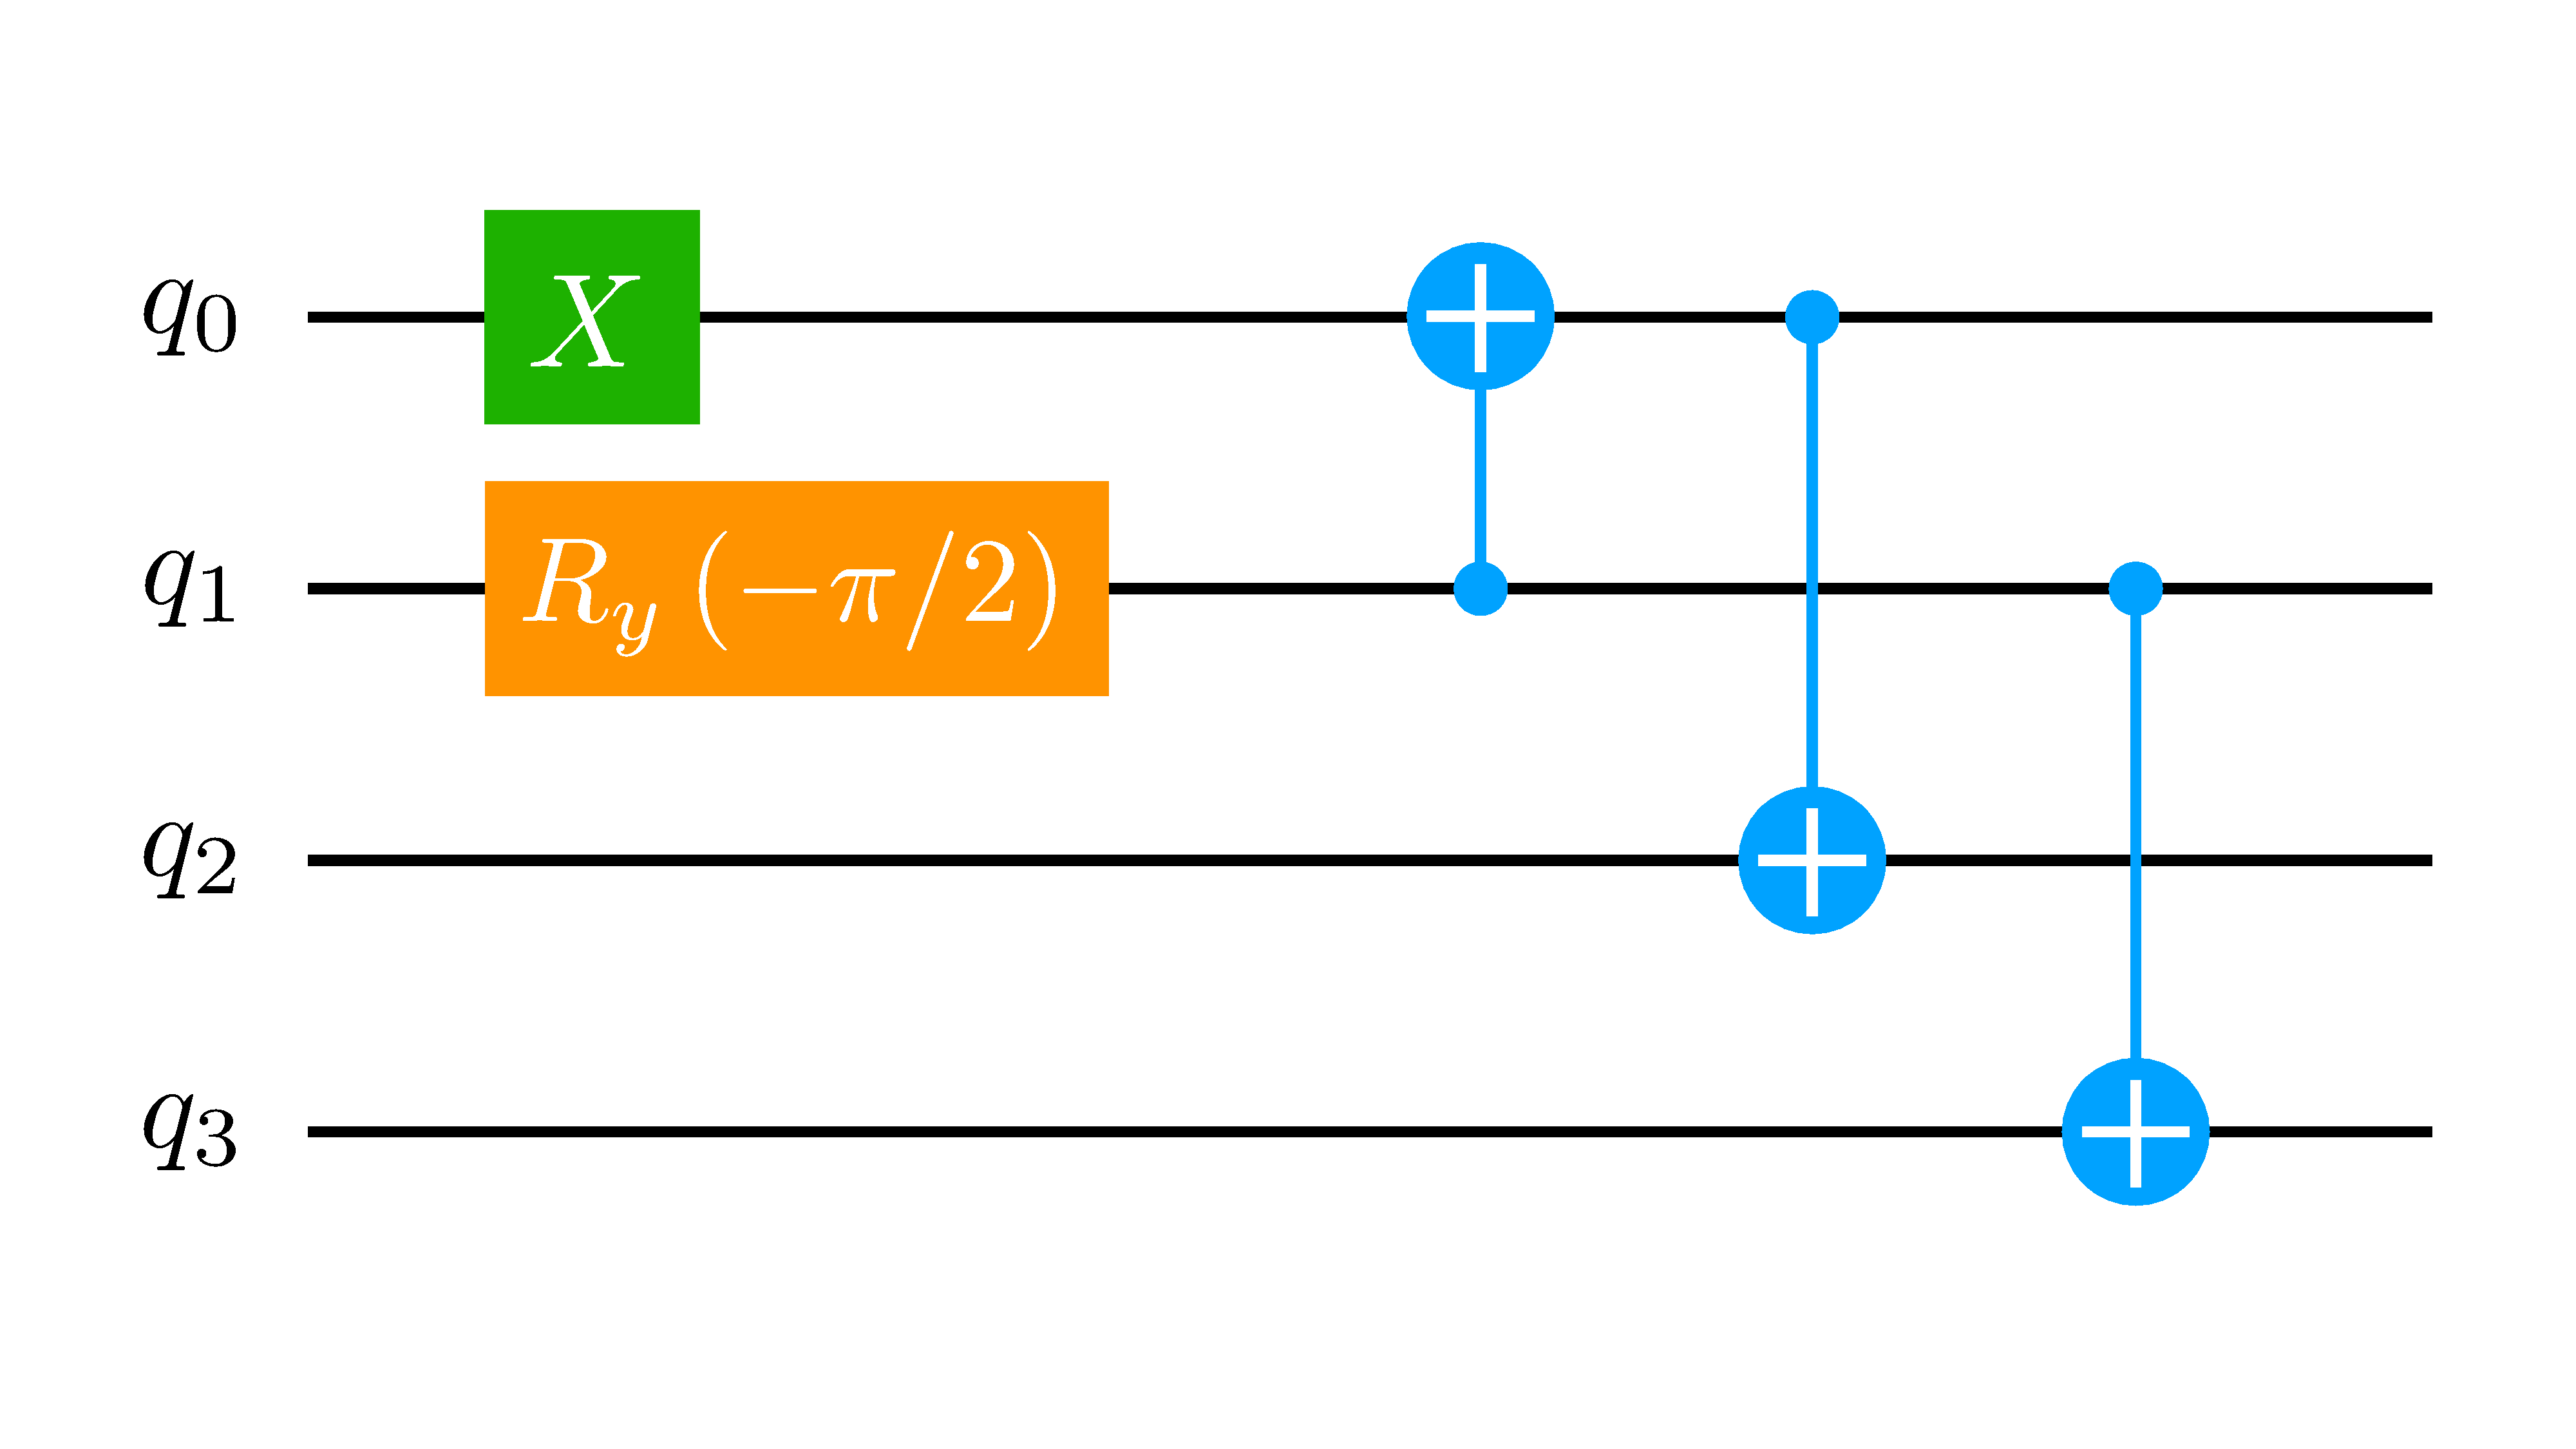
\includegraphics[width=\linewidth]{Figures/NJL1-model-solving/ansatz-implementation-base-state-preparation-gamma}
		\end{minipage}
	  \hspace{.025\linewidth}
		\begin{minipage}[c]{.45\linewidth}
			\centering
			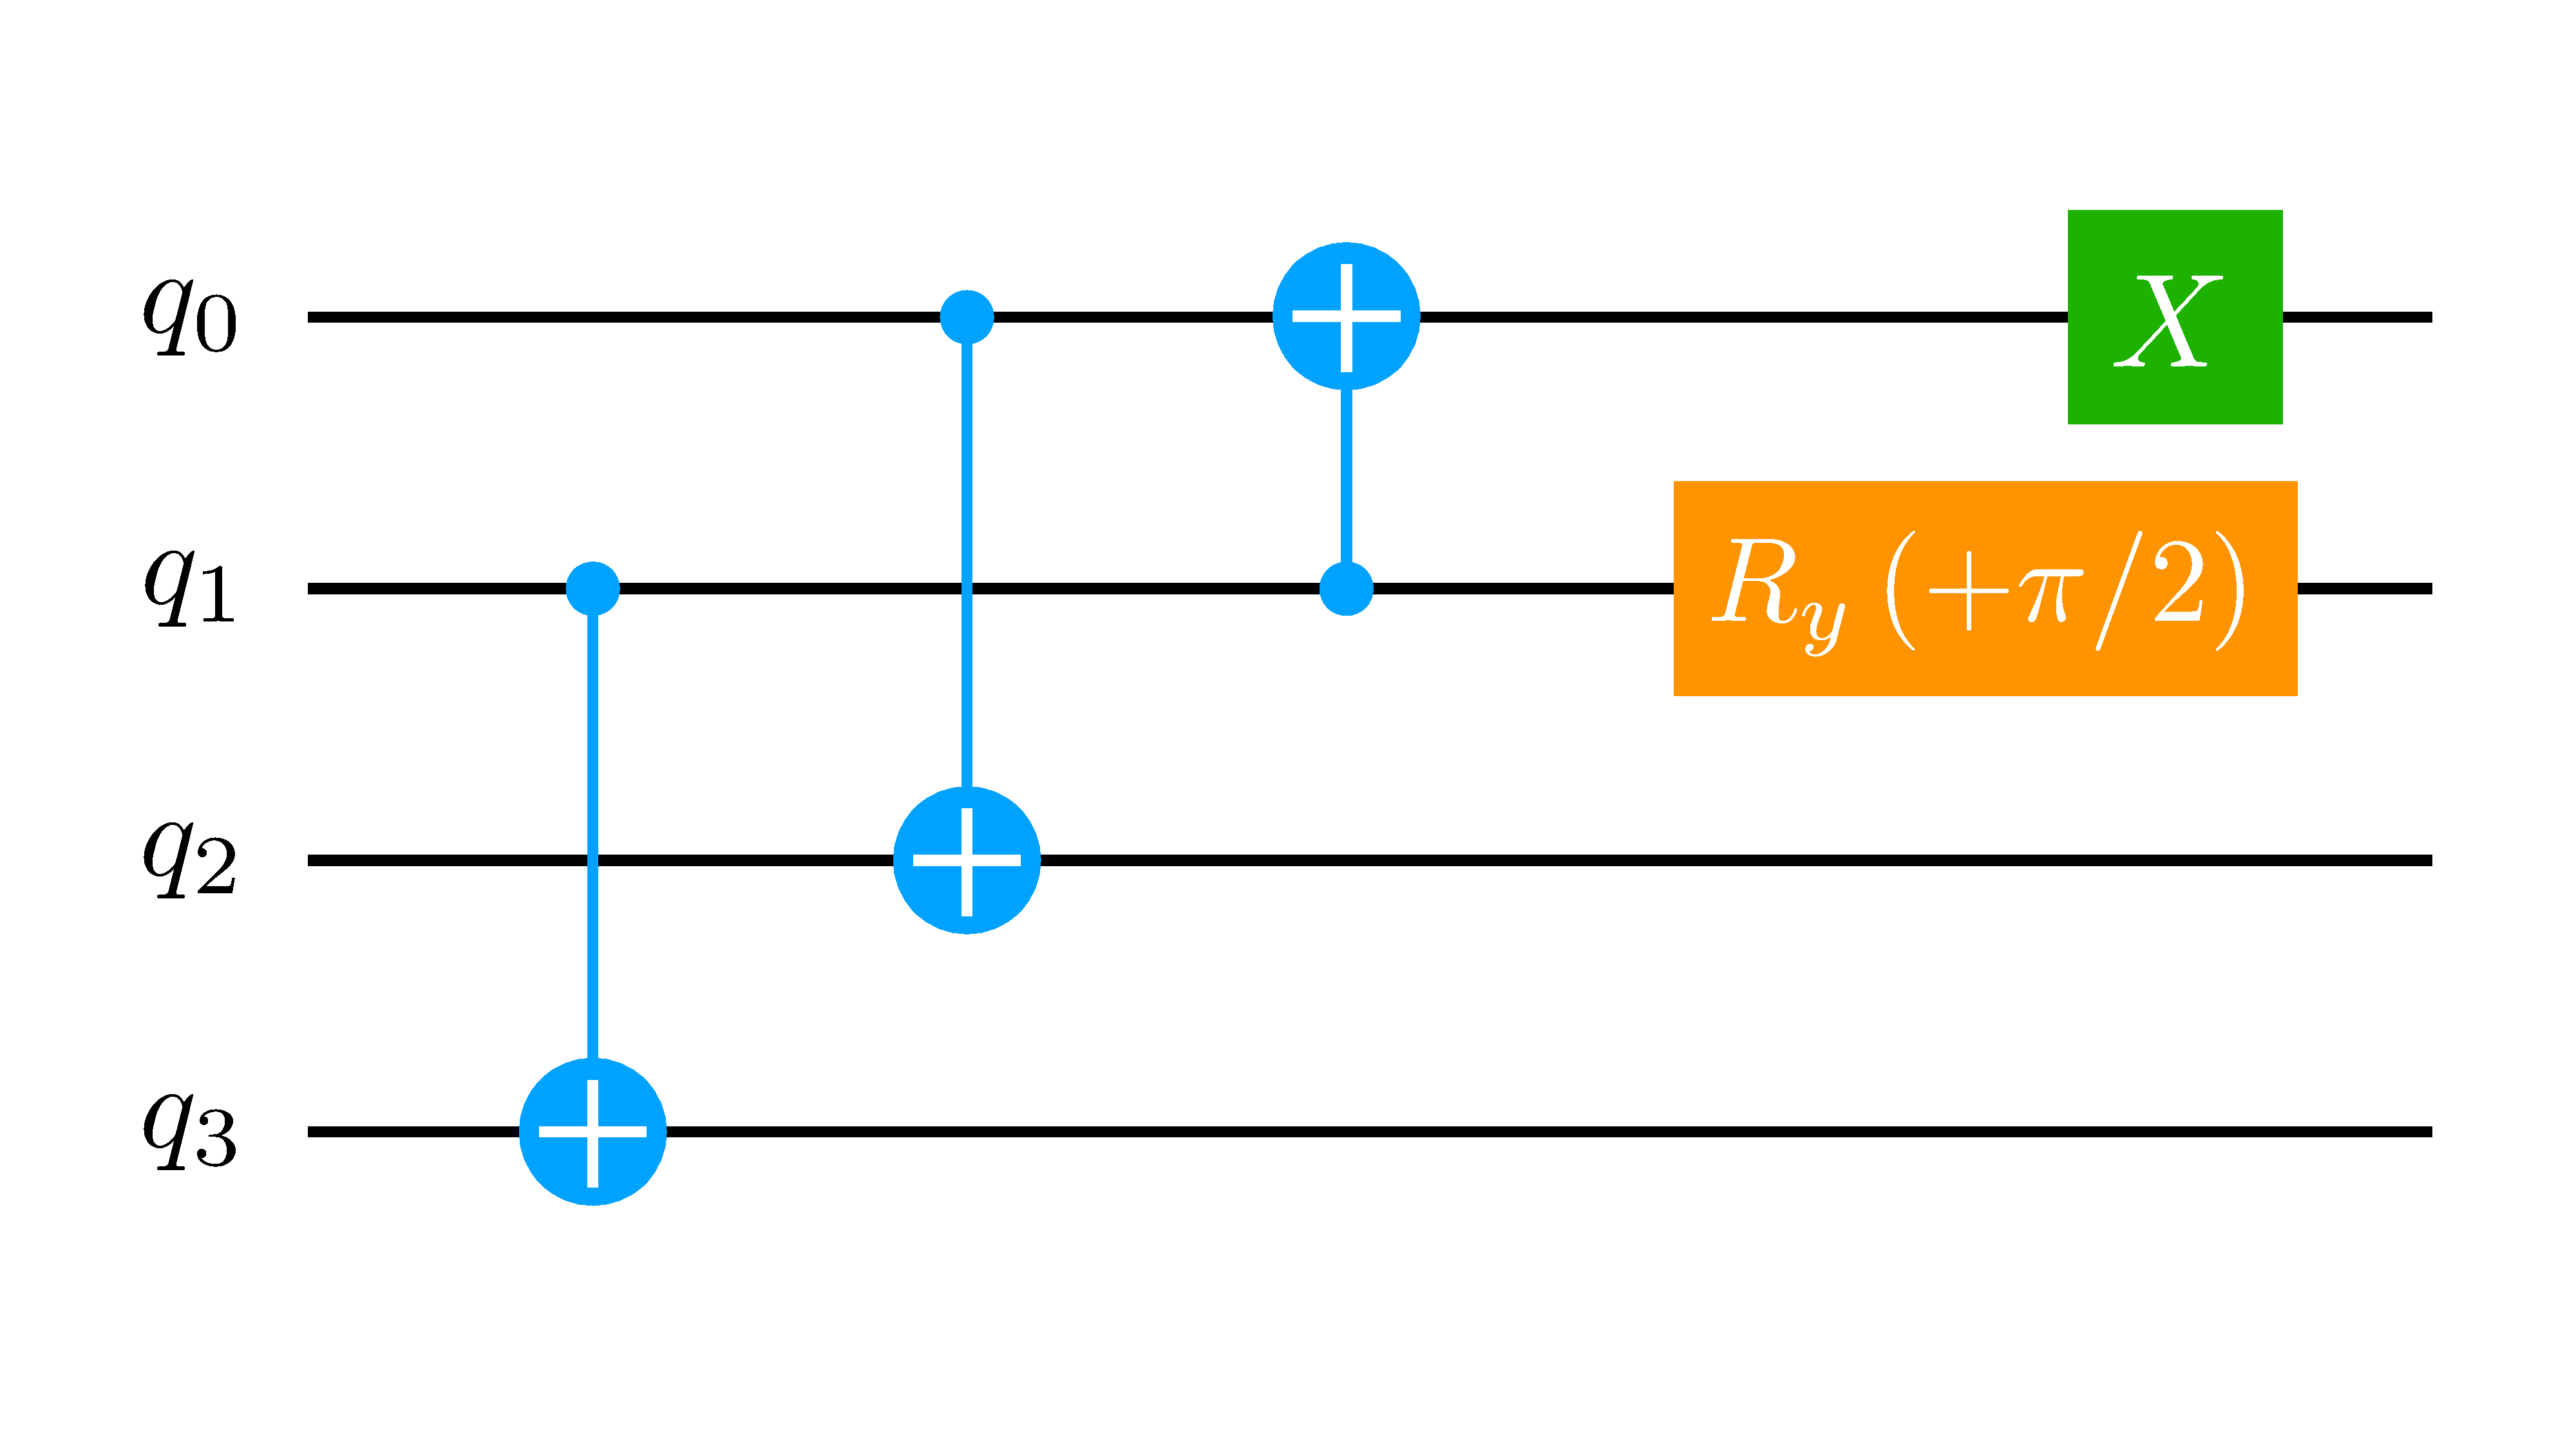
\includegraphics[width=\linewidth]{Figures/NJL1-model-solving/ansatz-implementation-base-state-reversing-gamma}
		\end{minipage}
		\caption{(Left) Preparation $\Gamma$ of state $\ket{\gamma}$. (Right) Quantum gate $\Gamma^{-1}$ for reversing state $\ket{\gamma}$.}
	\end{figure}

\break

	\begin{figure}[!p]
		\centering
		\begin{minipage}[c]{.45\linewidth}
			\centering
			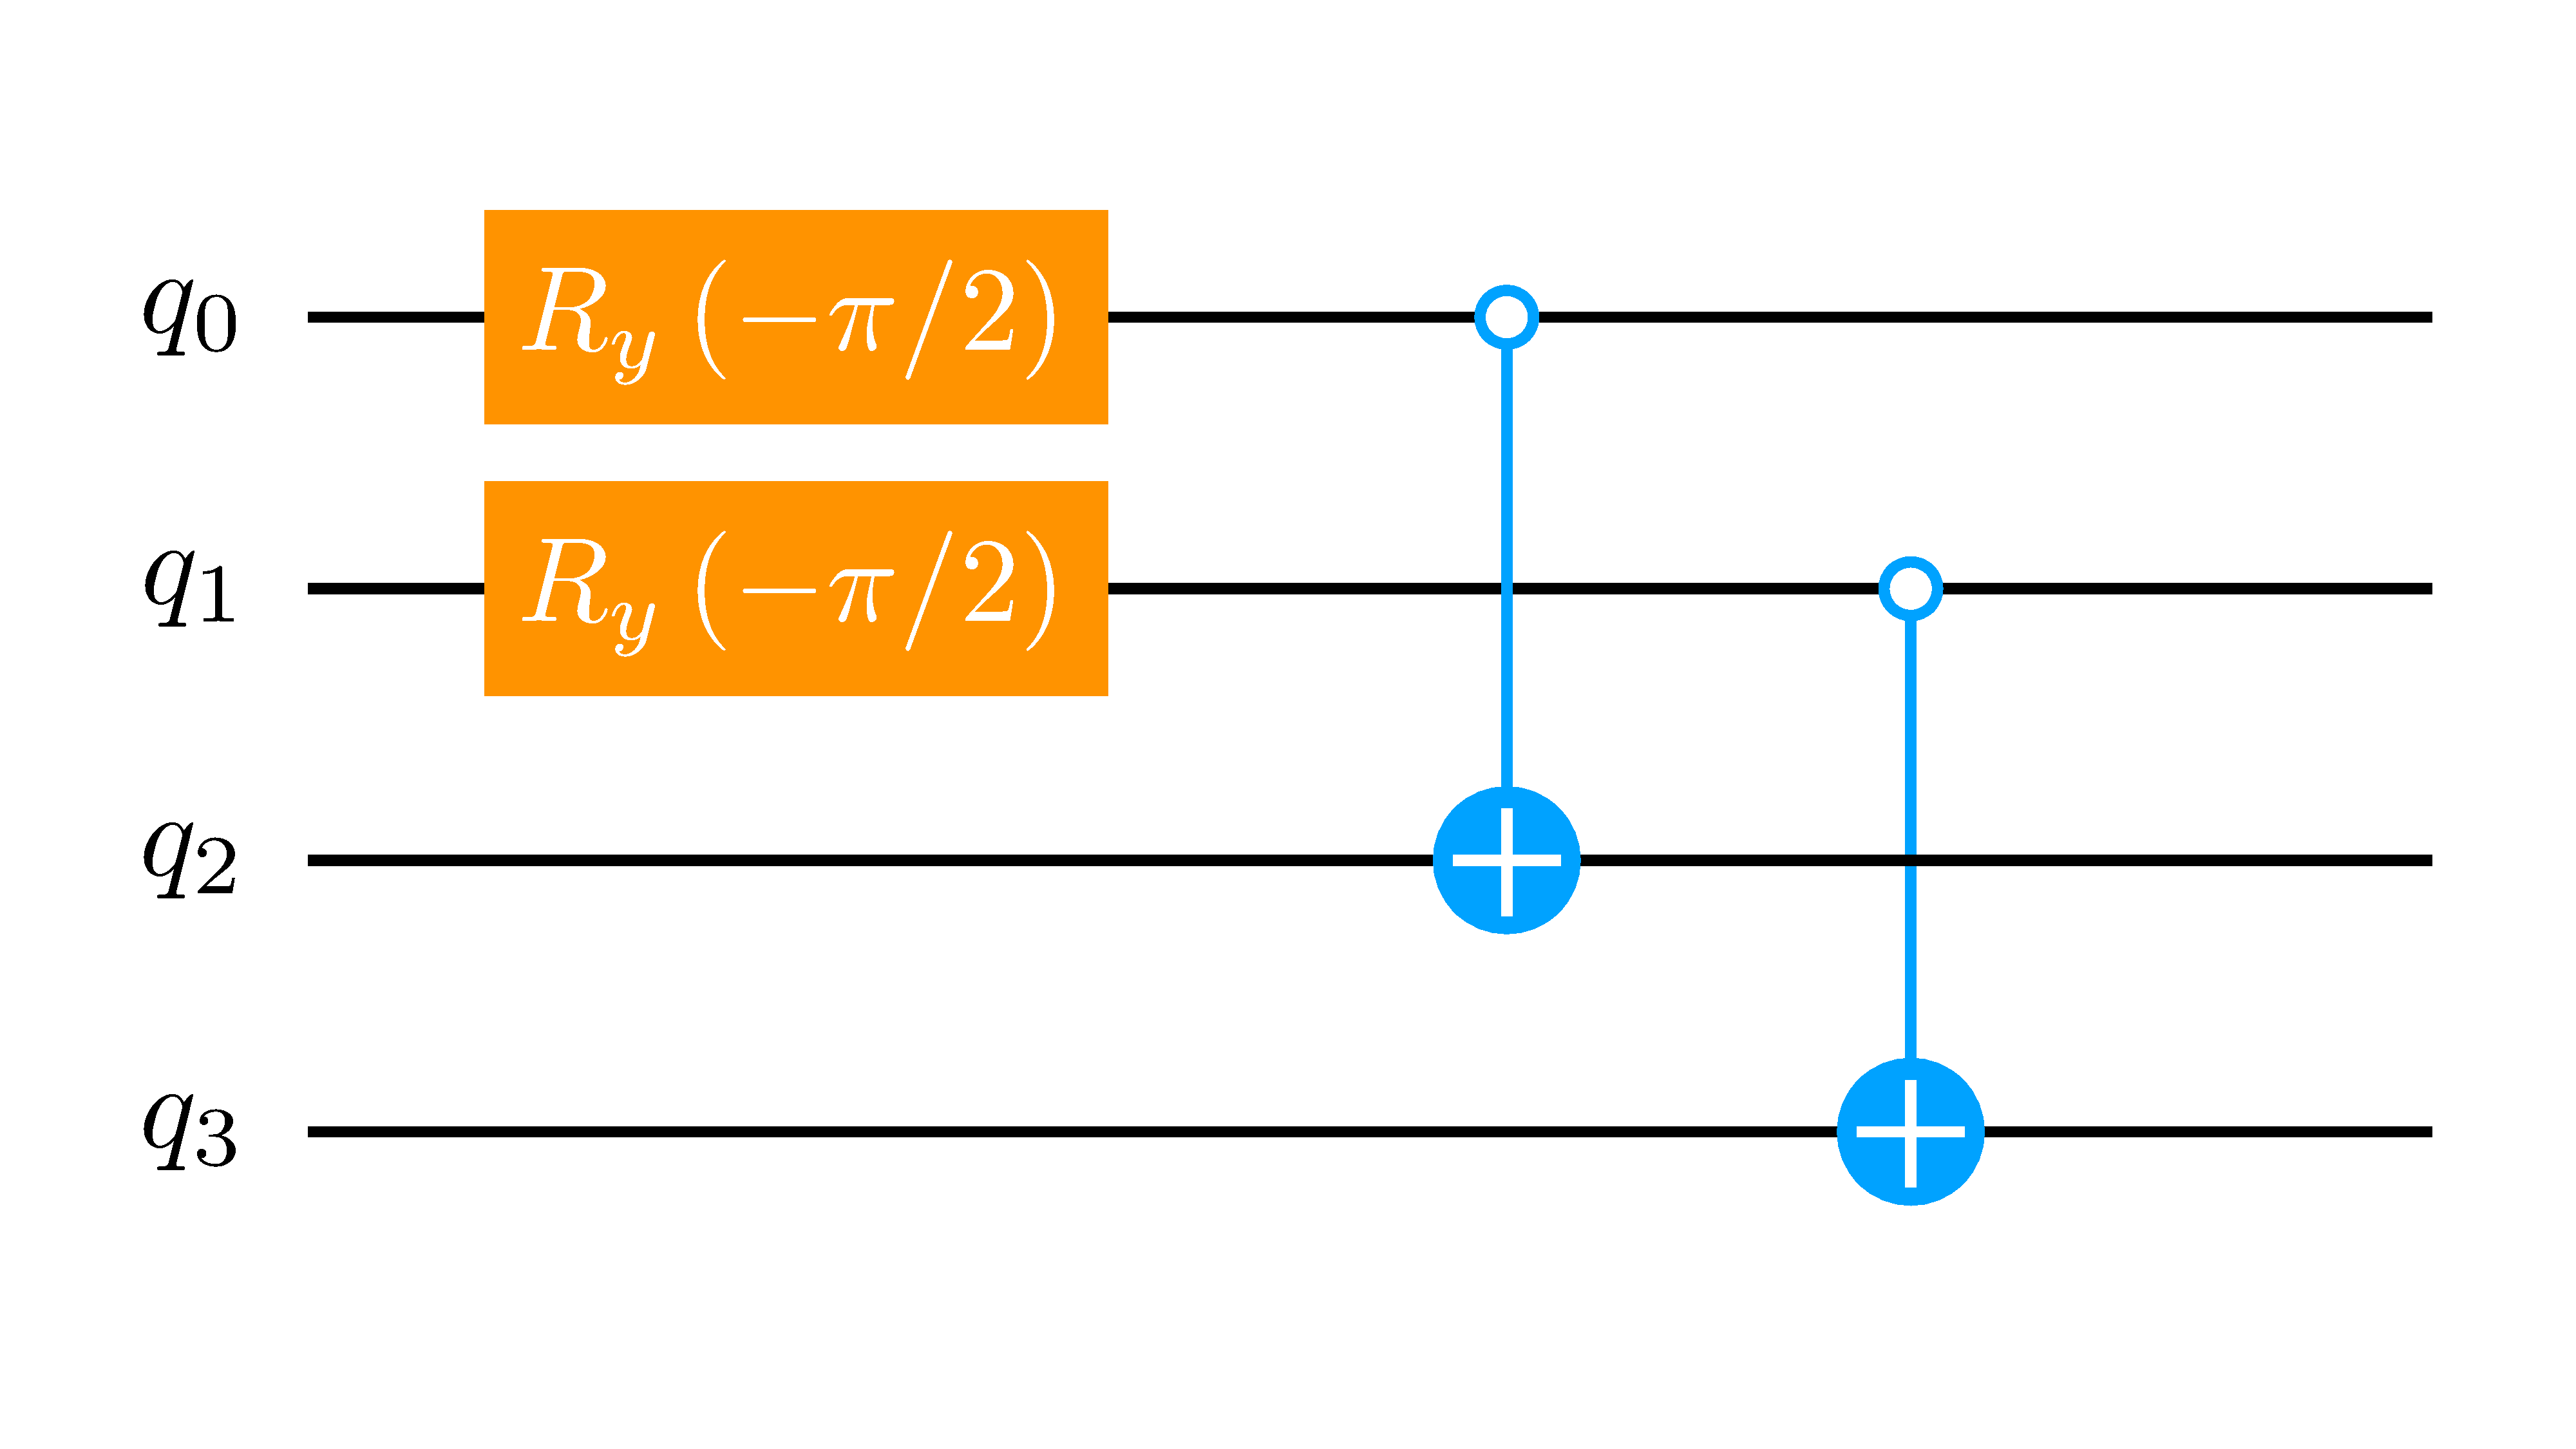
\includegraphics[width=\linewidth]{Figures/NJL1-model-solving/ansatz-implementation-base-state-preparation-kappa}
		\end{minipage}
	  \hspace{.025\linewidth}
		\begin{minipage}[c]{.45\linewidth}
			\centering
			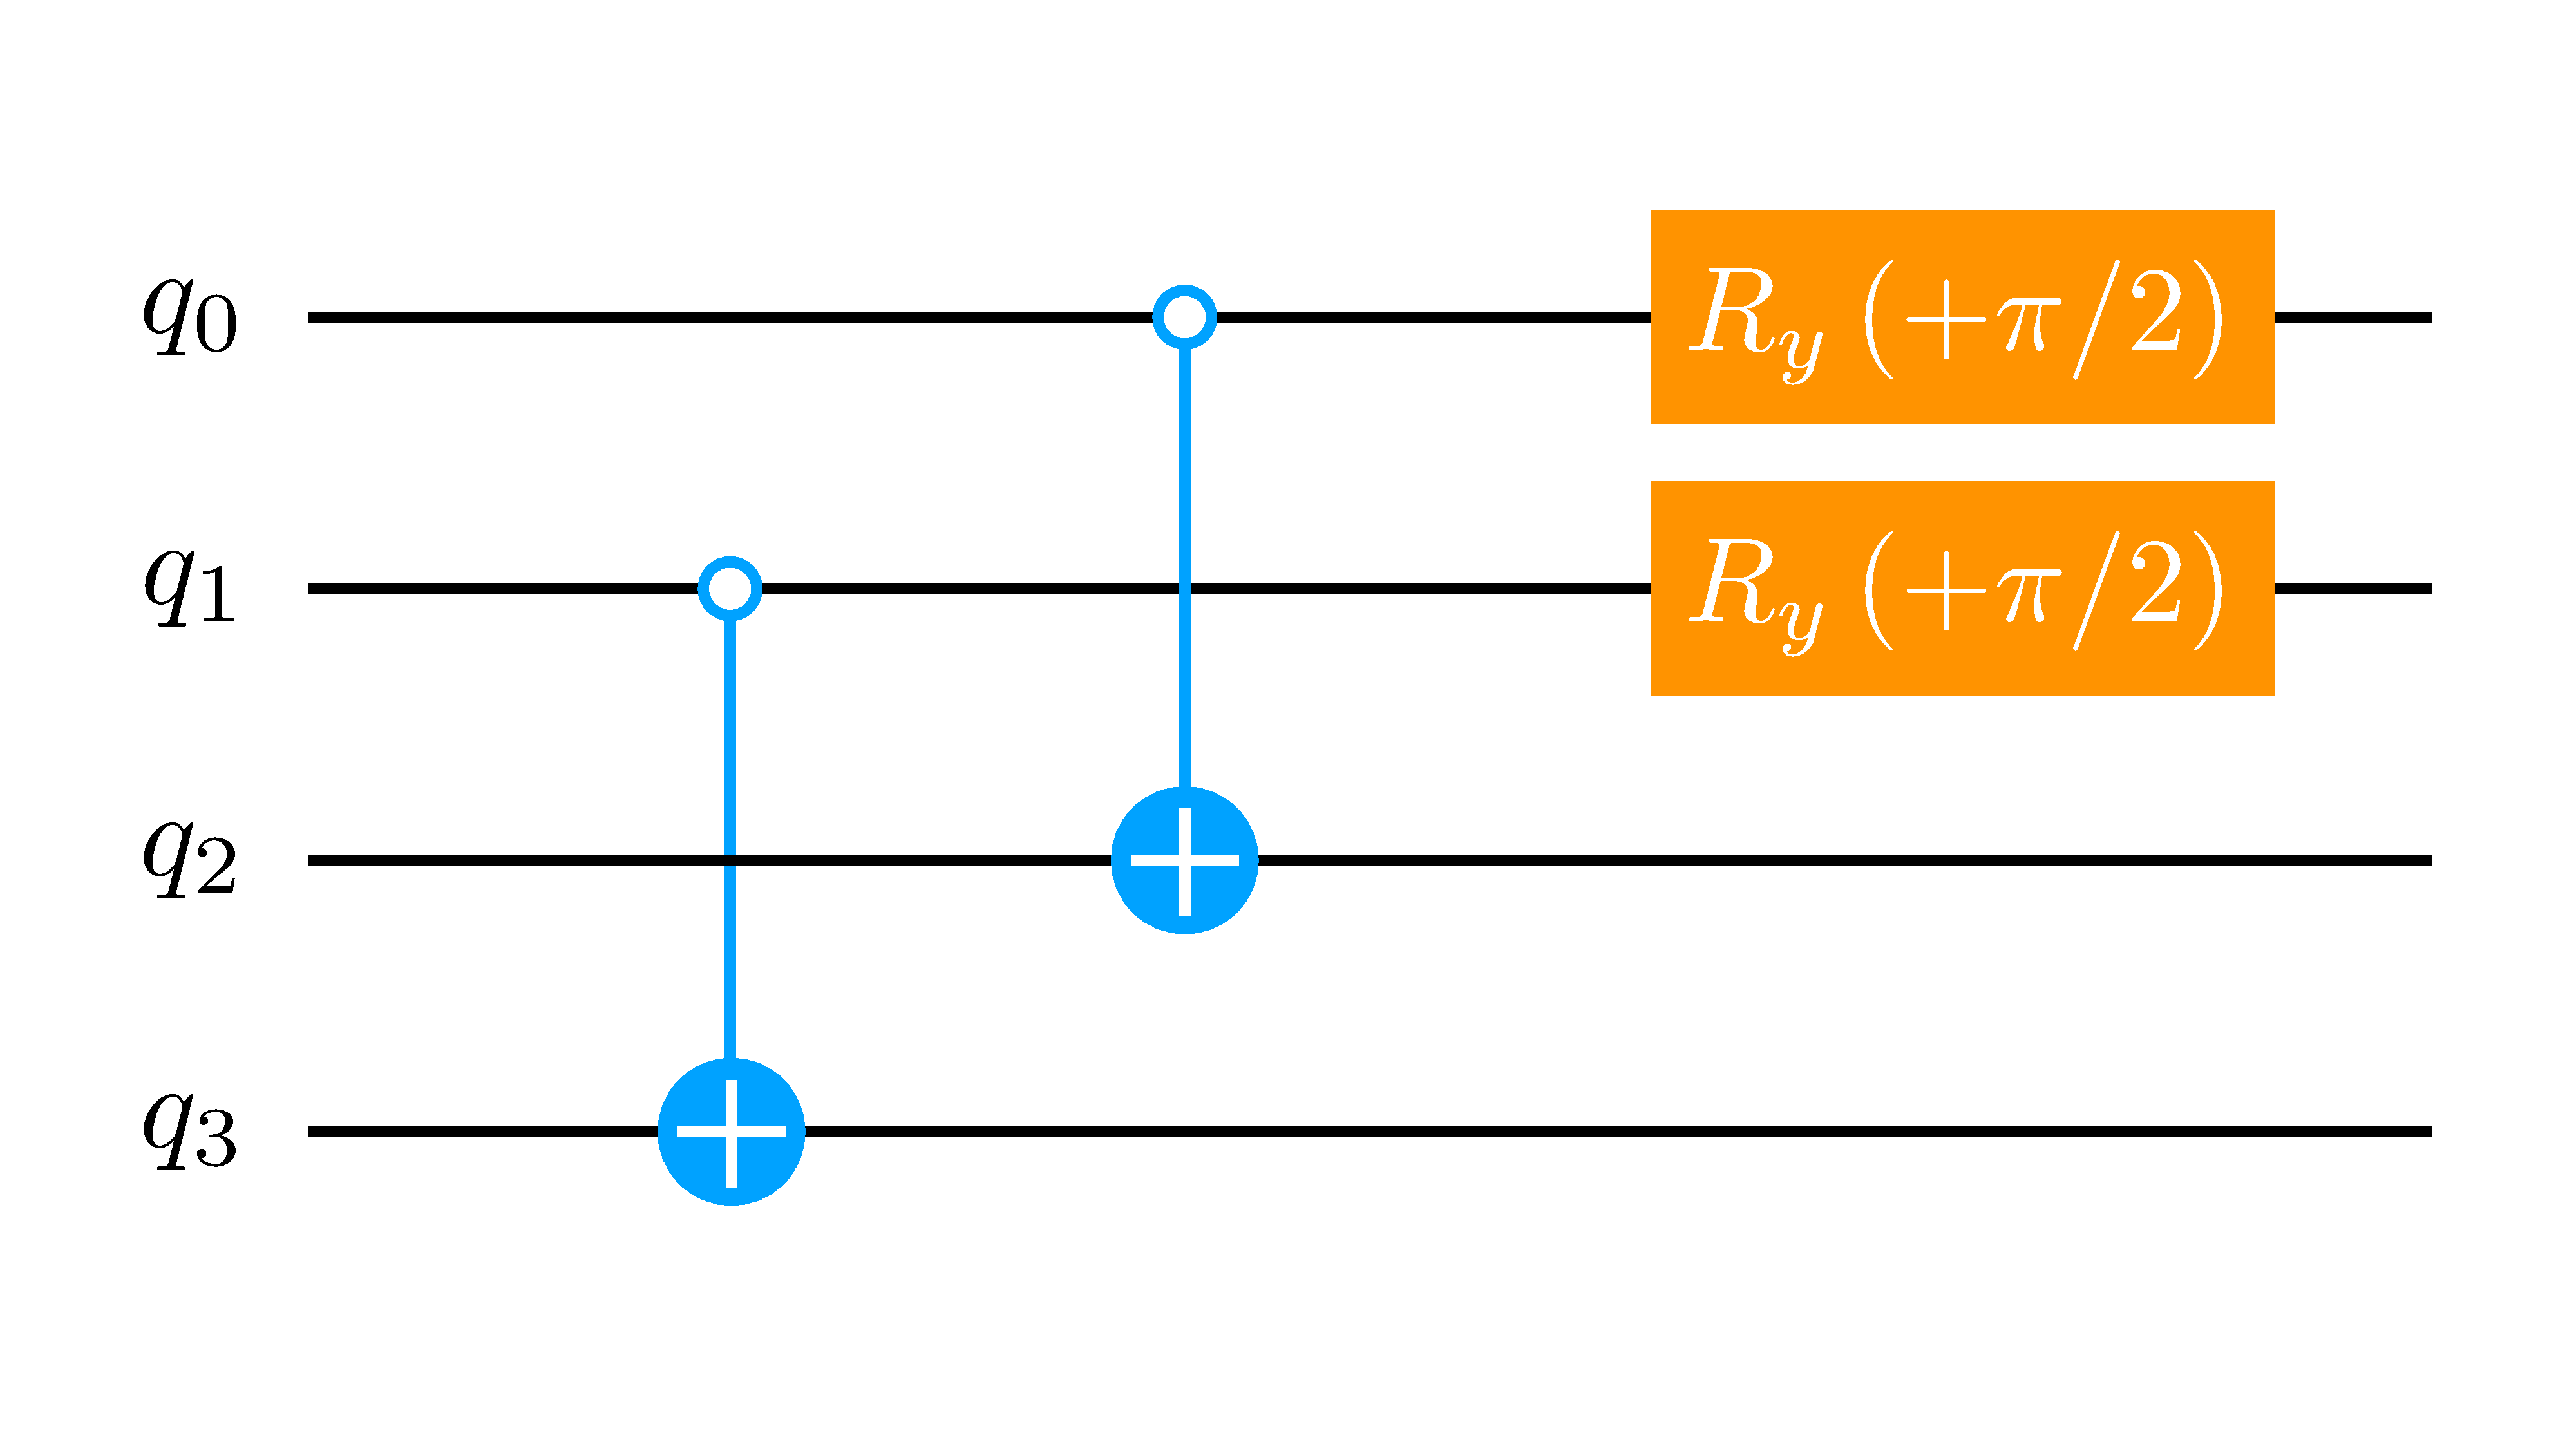
\includegraphics[width=\linewidth]{Figures/NJL1-model-solving/ansatz-implementation-base-state-reversing-kappa}
		\end{minipage}
		\caption{(Left) Preparation $\mathcal{K}$ of state $\ket{\kappa}$. (Right) Quantum gate $\mathcal{K}^{-1}$ for reversing state $\ket{\kappa}$.}
	\end{figure}

\break

	\begin{multicols}{2}

		This parametrization will work if we are interested in measuring in the computational basis only (i.e. Pauli-Z measurements). Nonetheless, if we change our basis before measuring (e.g. to Pauli-X or Pauli-Y) we are going to face a problem: the resulting states of our system will be entangled with the ancilla qubit, and so, states that should be indistinguishable from one another will turn out distinct; because of this, the probability distributions will not be correct.

		\begin{gather*}
		  \text{Pr} \qty(\ket{\psi}_{\text{distinct}}) =
		    \norm{\psi_\gamma}^2 + \norm{\psi_\kappa}^2 \\
		  \text{Pr} \qty(\ket{\psi}_{\text{indist}}) =
		    \norm{\psi_\gamma + \psi_\kappa}^2 \\
		  \text{Pr} \qty(\ket{\psi}_{\text{distinct}}) \geq
		    \text{Pr} \qty(\ket{\psi}_{\text{indist}})
		\end{gather*}

		\columnbreak

		Therefore, as a last step, we need to \textbf{break this entanglement}.

		\begin{center}
			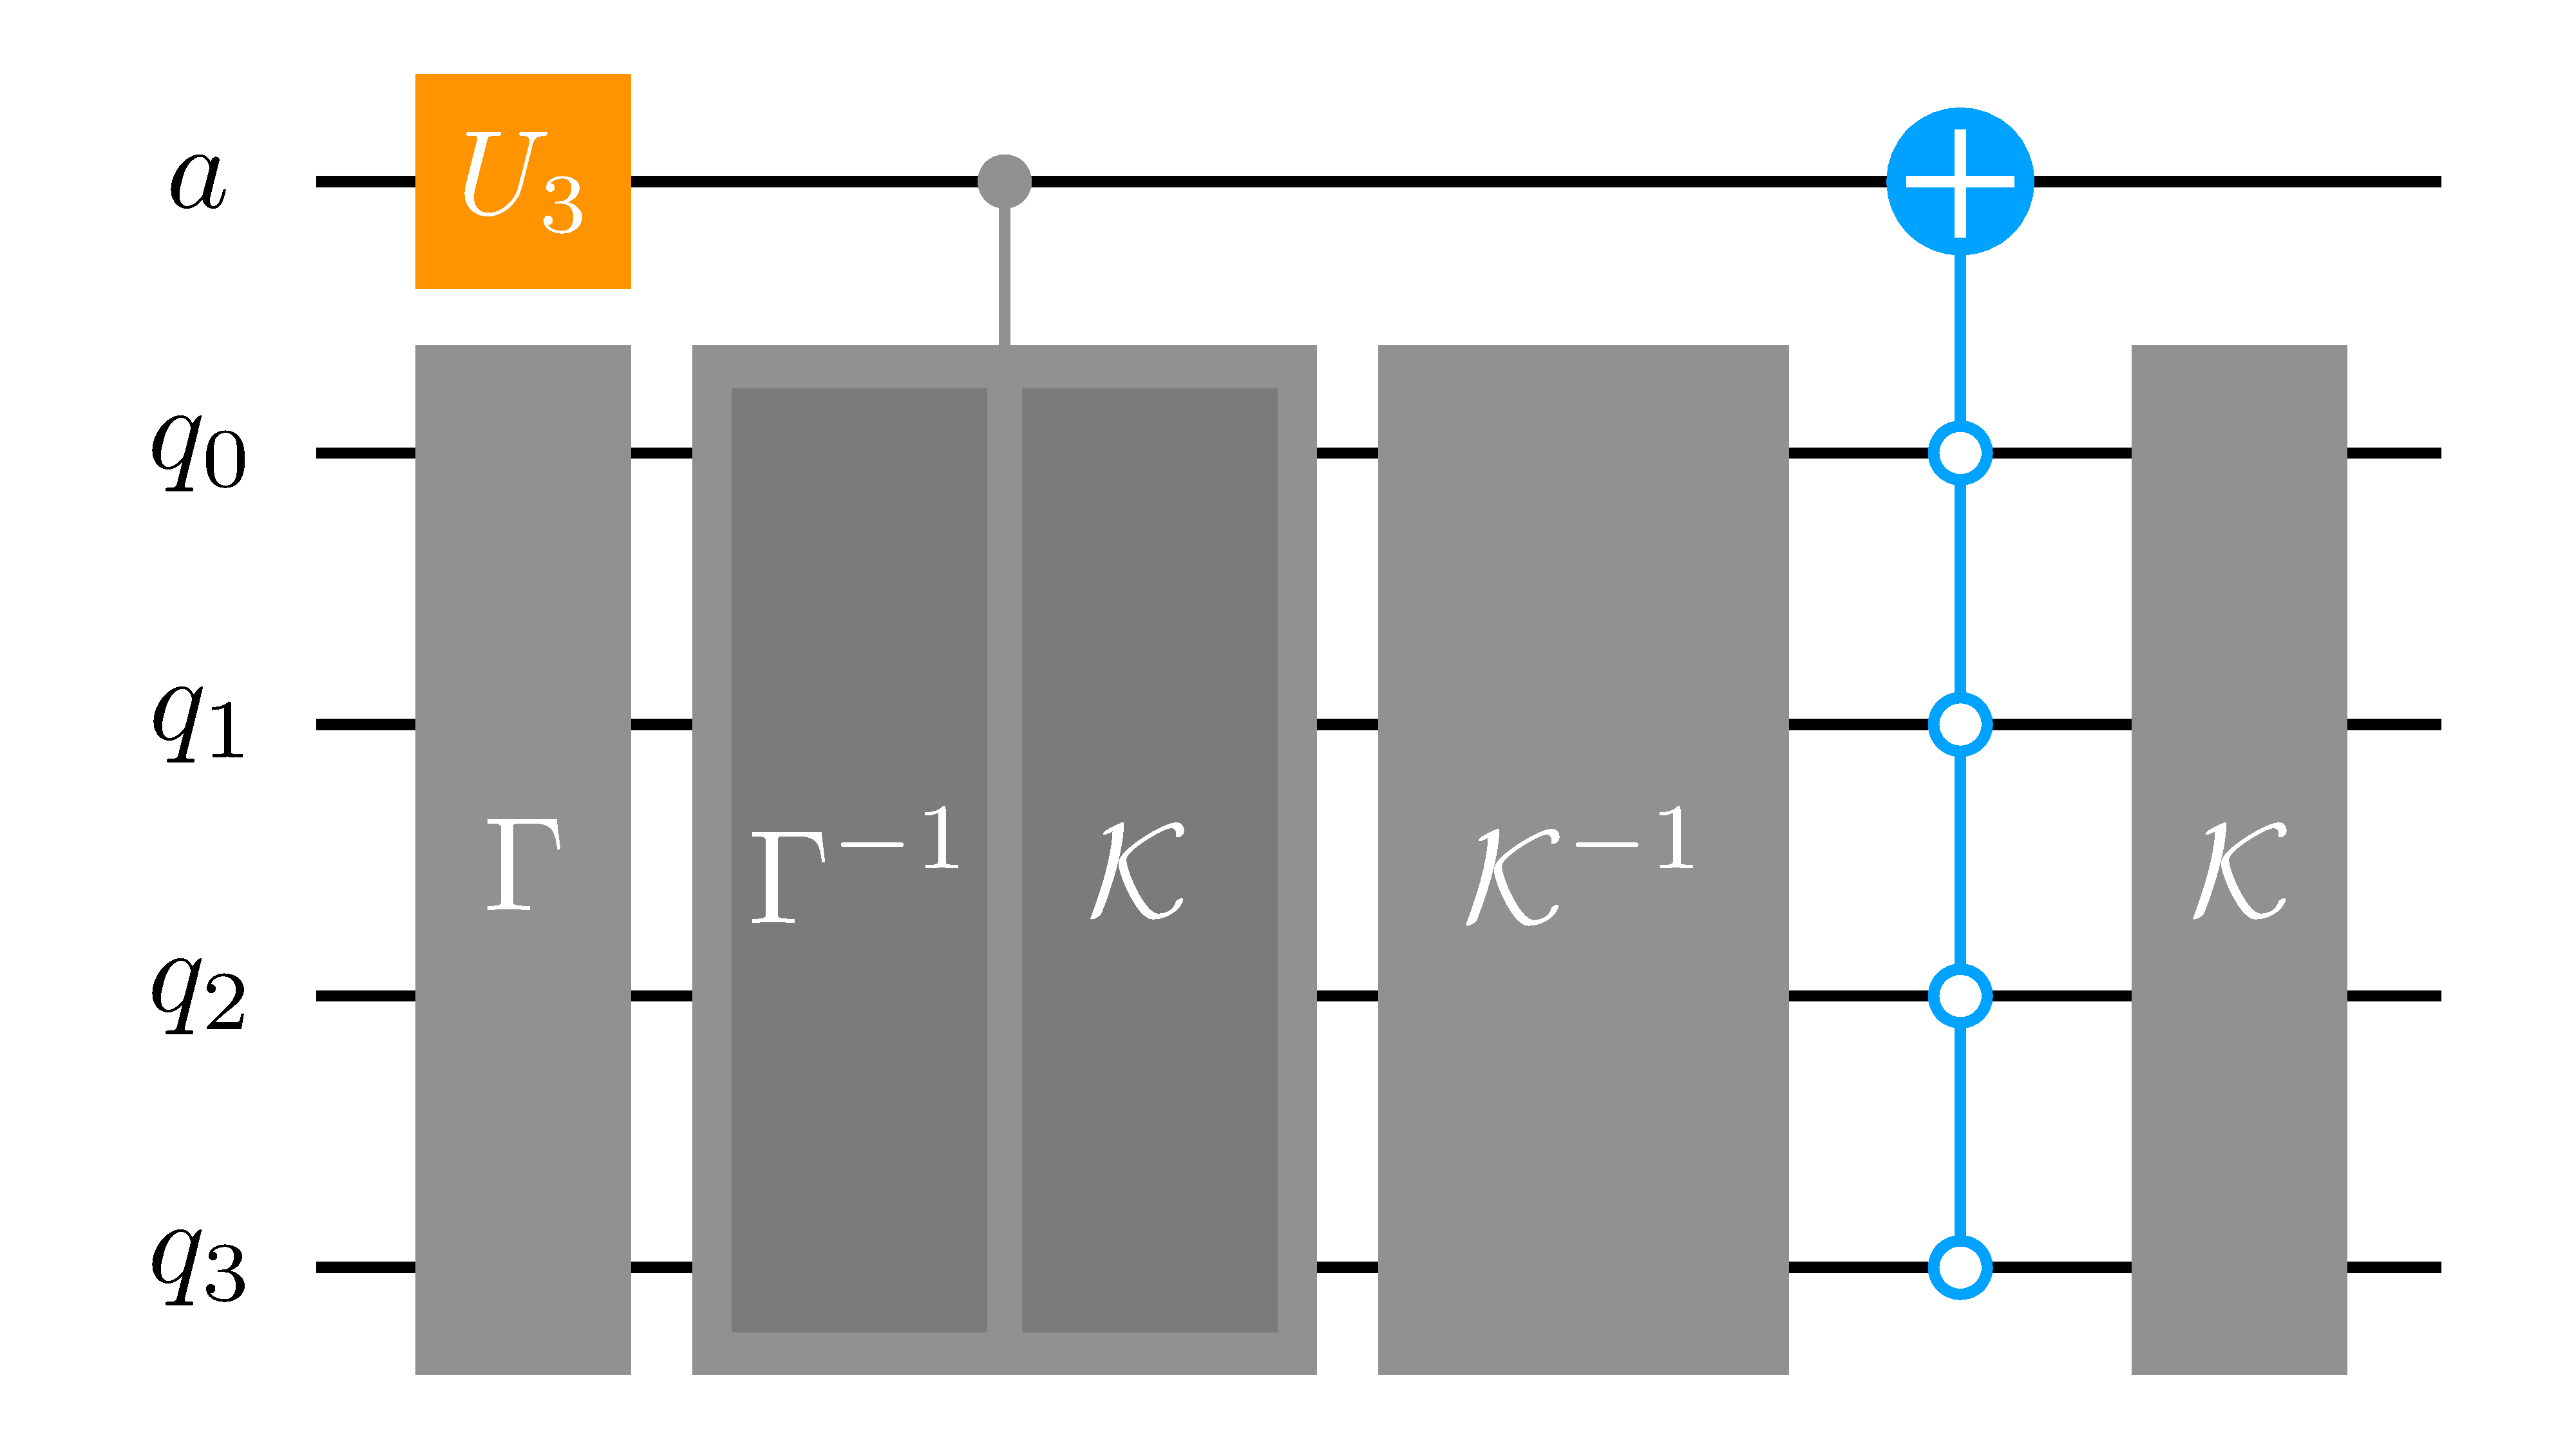
\includegraphics[width=.4\paperwidth]{Figures/NJL1-model-solving/ansatz-implementation-circuit}
		\end{center}

	\end{multicols}

\end{frame}

%% ----------------------------------------------------------------------------

\subsection{Ground state energy}

\begin{frame}[allowframebreaks]{Variational quantum eigensolver algorithm}

	We can now solve for the ground state energy of our system. This can be accomplished by making use of the hybrid quantum-classical algorithm known as the \textbf{Variational Quantum Eigensolver} (VQE); which is based in the \textbf{variational theorem of quantum mechanics}:

	\begin{gather*}
	  \ev{H}\!\qty(\theta^{n}) \equiv
	    \ev{H}{\psi\qty(\theta^{n})} \geq
	    \lambda_{\text{min}}
	\end{gather*}

	Evaluating the expectation value of the different components making up our Hamiltonian is done through a process known as \textbf{operator averaging}:

	\begin{gather*}
	  P_{N} = \sum_{p=1}^{\order{N^q}} w_{p} P_{N}^{p} \qRa
	  \ev{P_{N}} = \sum_{p=1}^{\order{N^q}} w_{p} \ev{P_{N}^{p}}
	\end{gather*}

\break

	\begin{center}
		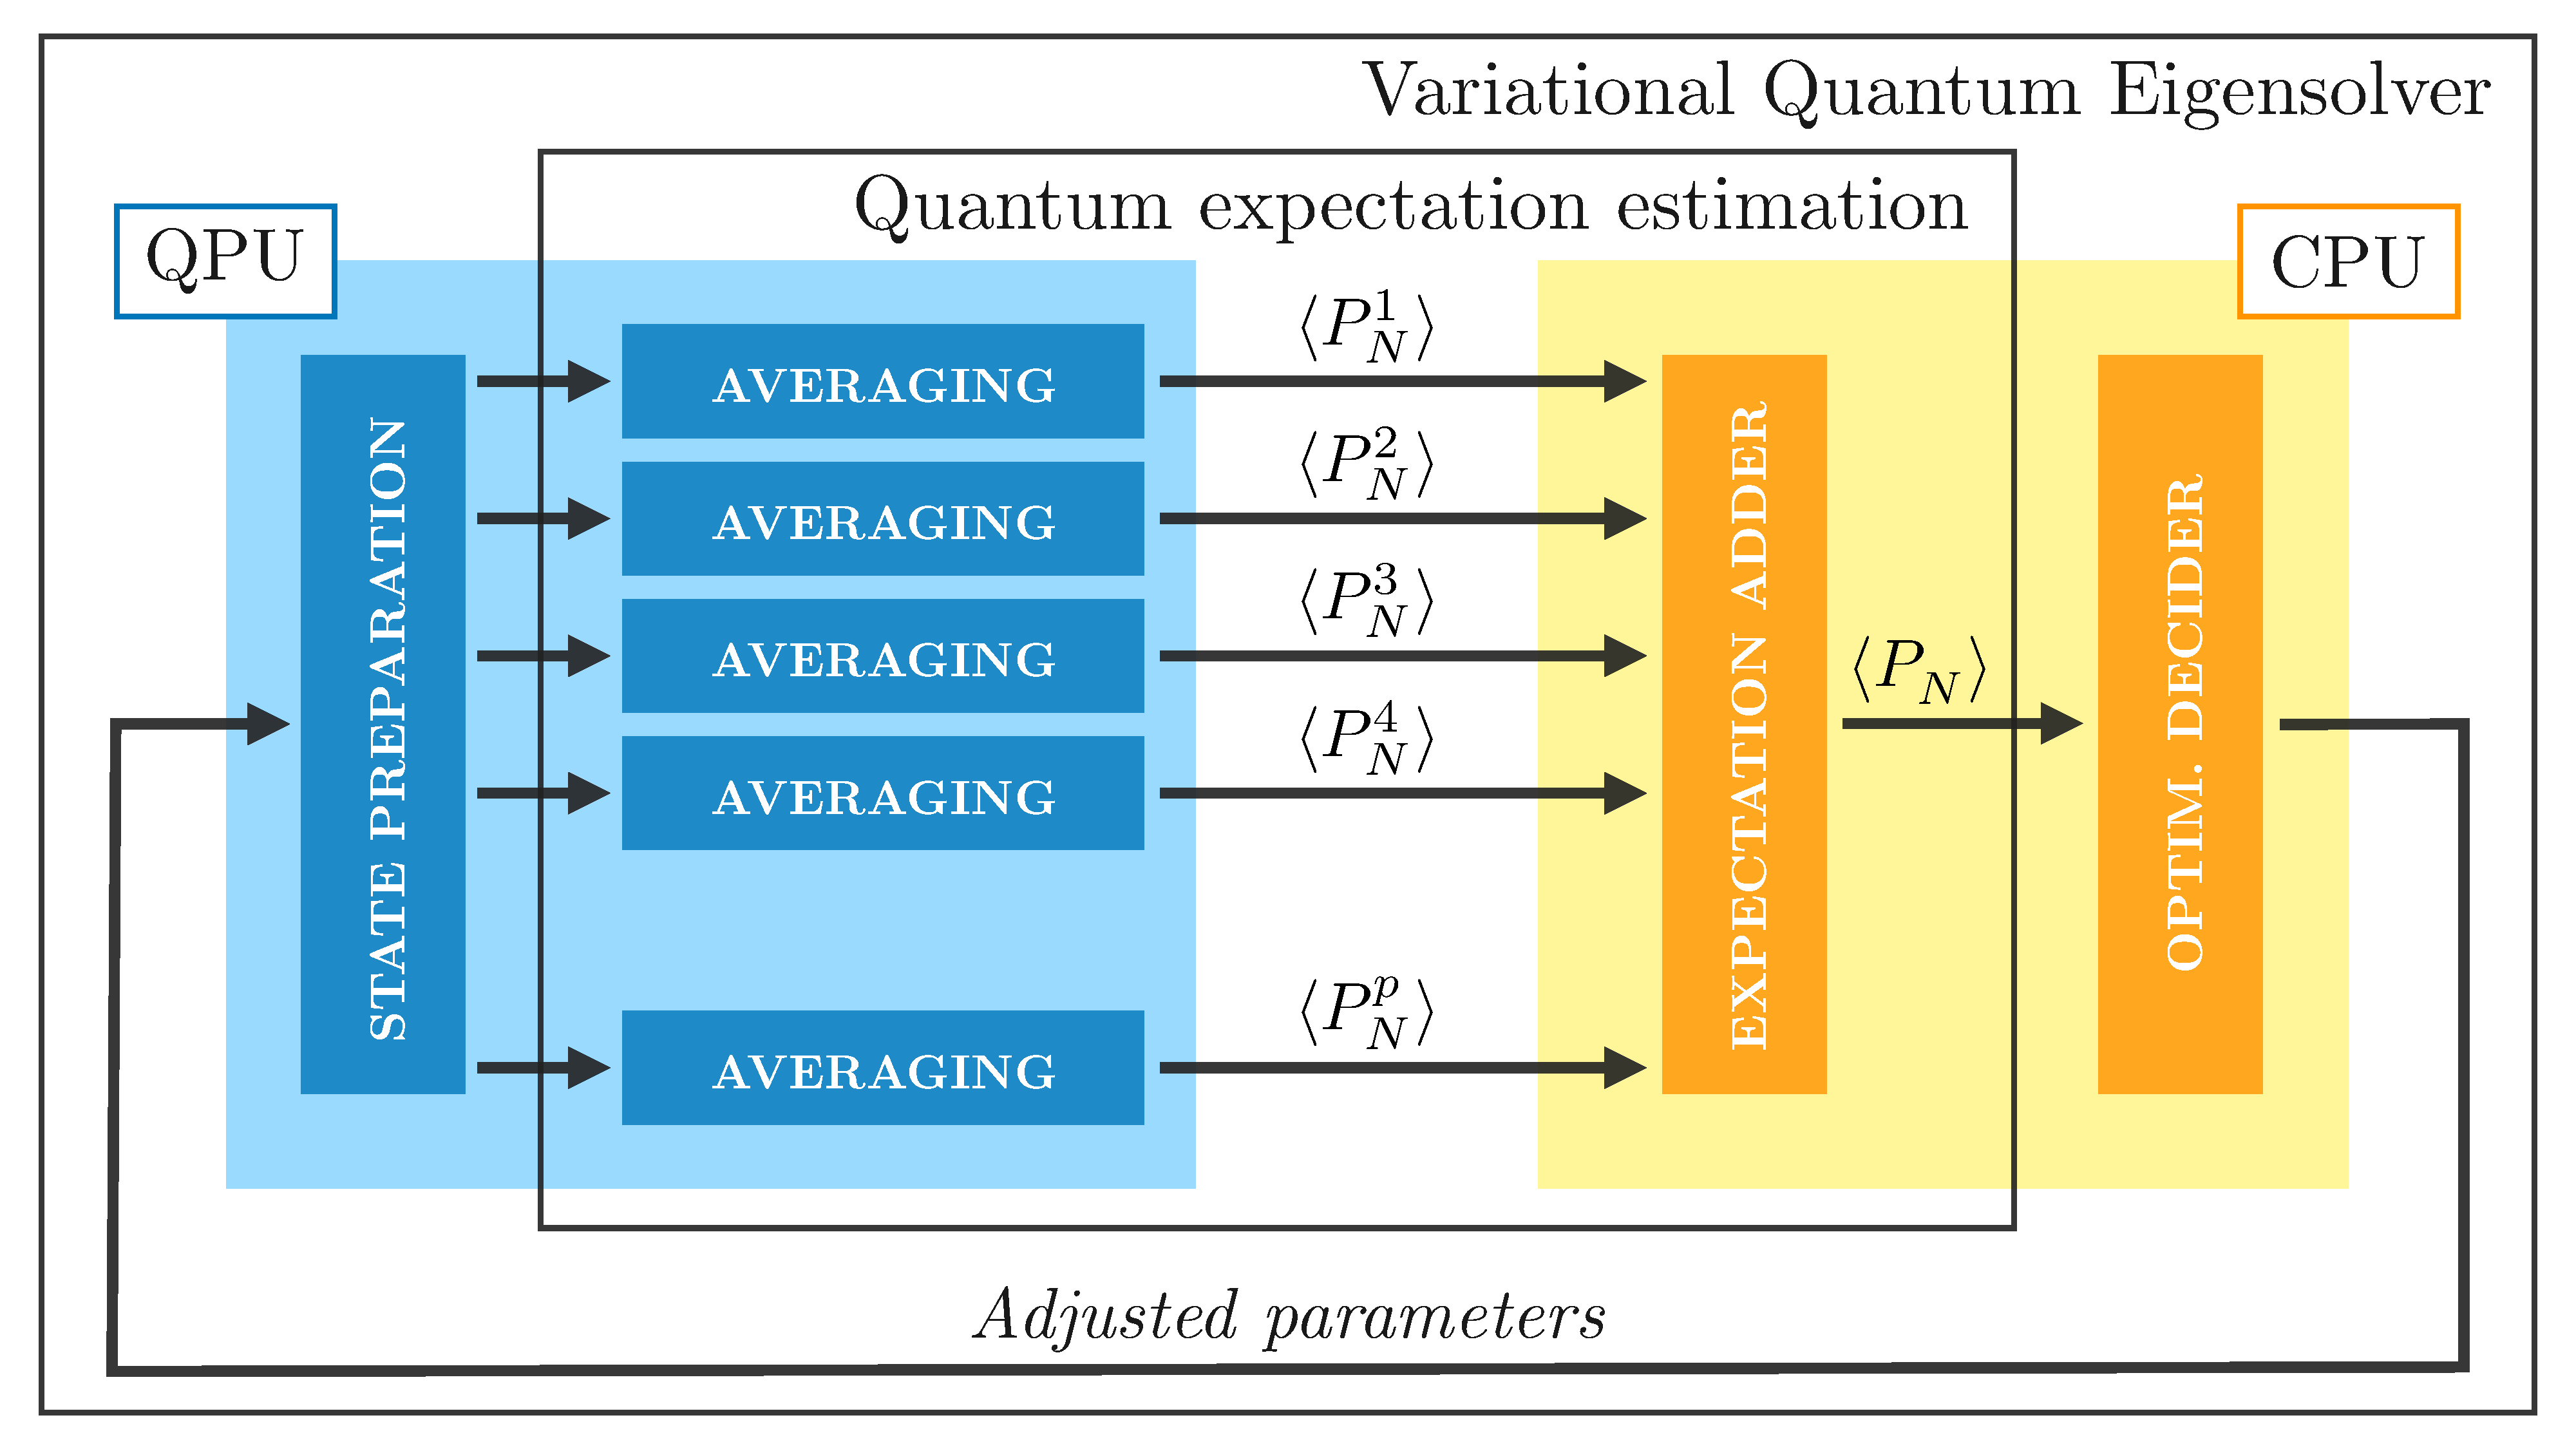
\includegraphics[width=.7\paperwidth]{Figures/NJL1-model-solving/VQE}
	\end{center}

\end{frame}

%% ----------------------------------------------------------------------------

\begin{frame}[allowframebreaks]{Optimal sampling regression algorithm}

	The method that we have used to parametrize space will naturally return cycles in the the states that we are parametrizing. Such \textbf{periodic nature} will transfer to the expectation value function, which in turn allows us to consistently apply Fourier analysis to fully describe it:

	\begin{gather*}
	  f(\theta) \equiv a_0 + \sum_{s=1}^S \qty[a_s\cos(s\theta) + b_s\sin(s\theta)] \\
	  \mqty[
	    1 & \cos(\theta_1) & \sin(\theta_1) & \cos(2\theta_1)
	      & \cdots & \sin(S\theta_1) \\
	    1 & \cos(\theta_2) & \sin(\theta_2) & \cos(2\theta_2)
	      & \cdots & \sin(S\theta_2) \\
	    \vdots & \vdots & \vdots & \vdots & \ddots & \vdots \\
	    1 & \cos(\theta_{2S+1}) & \sin(\theta_{2S+1}) & \cos(2\theta_{2S+1})
	      & \cdots & \sin(S\theta_{2S+1})
	  ]
	  \mqty[
	    a_0 \\ a_1 \\ b_1 \\ a_2 \\ \vdots \\ b_S
	  ] =
	  \mqty[
	    f(\theta_1) \\ f(\theta_2) \\ \vdots \\ f(\theta_{2S+1})
	  ] \\[5pt]
	  Fc = f \qra F^{\dagger}Fc = F^{\dagger}f
	\end{gather*}

\break

	Generally $S \ra \infty$, however, if the bandwidth is bounded, $S$ will be finite and it will be possible to evaluate this expression exactly. Theoretically, the power of this method is demonstrated through the \textbf{Nyquist-Shannon sampling theorem}; which states that if a function $f(\theta)$ contains no angular frequencies higher than $\omega_{\text{S}}$, it is completely determined by giving its ordinates at a series of points $1/2\omega_{\text{S}}$ apart:

	\begin{gather*}
	  \omega_{\text{sampling}} > 2\omega_{\text{S}}
	\end{gather*}

	Extending these results to \textbf{higher dimensions} is straight forward considering multidimensional Fourier series. In this case, we may have a different bandwidth $S_{q}$ for each parameter. Calling the total number of parameters $Q$, and the maximum bandwidth $S_{\text{max}}$, the total number of samples $T$ required by this method is:

	\begin{gather*}
	  T = \prod_{q=1}^{Q} \qty(2 S_{q} + 1) = \order{S_{\text{max}}^{Q}}
	\end{gather*}

\break

	\begin{center}
		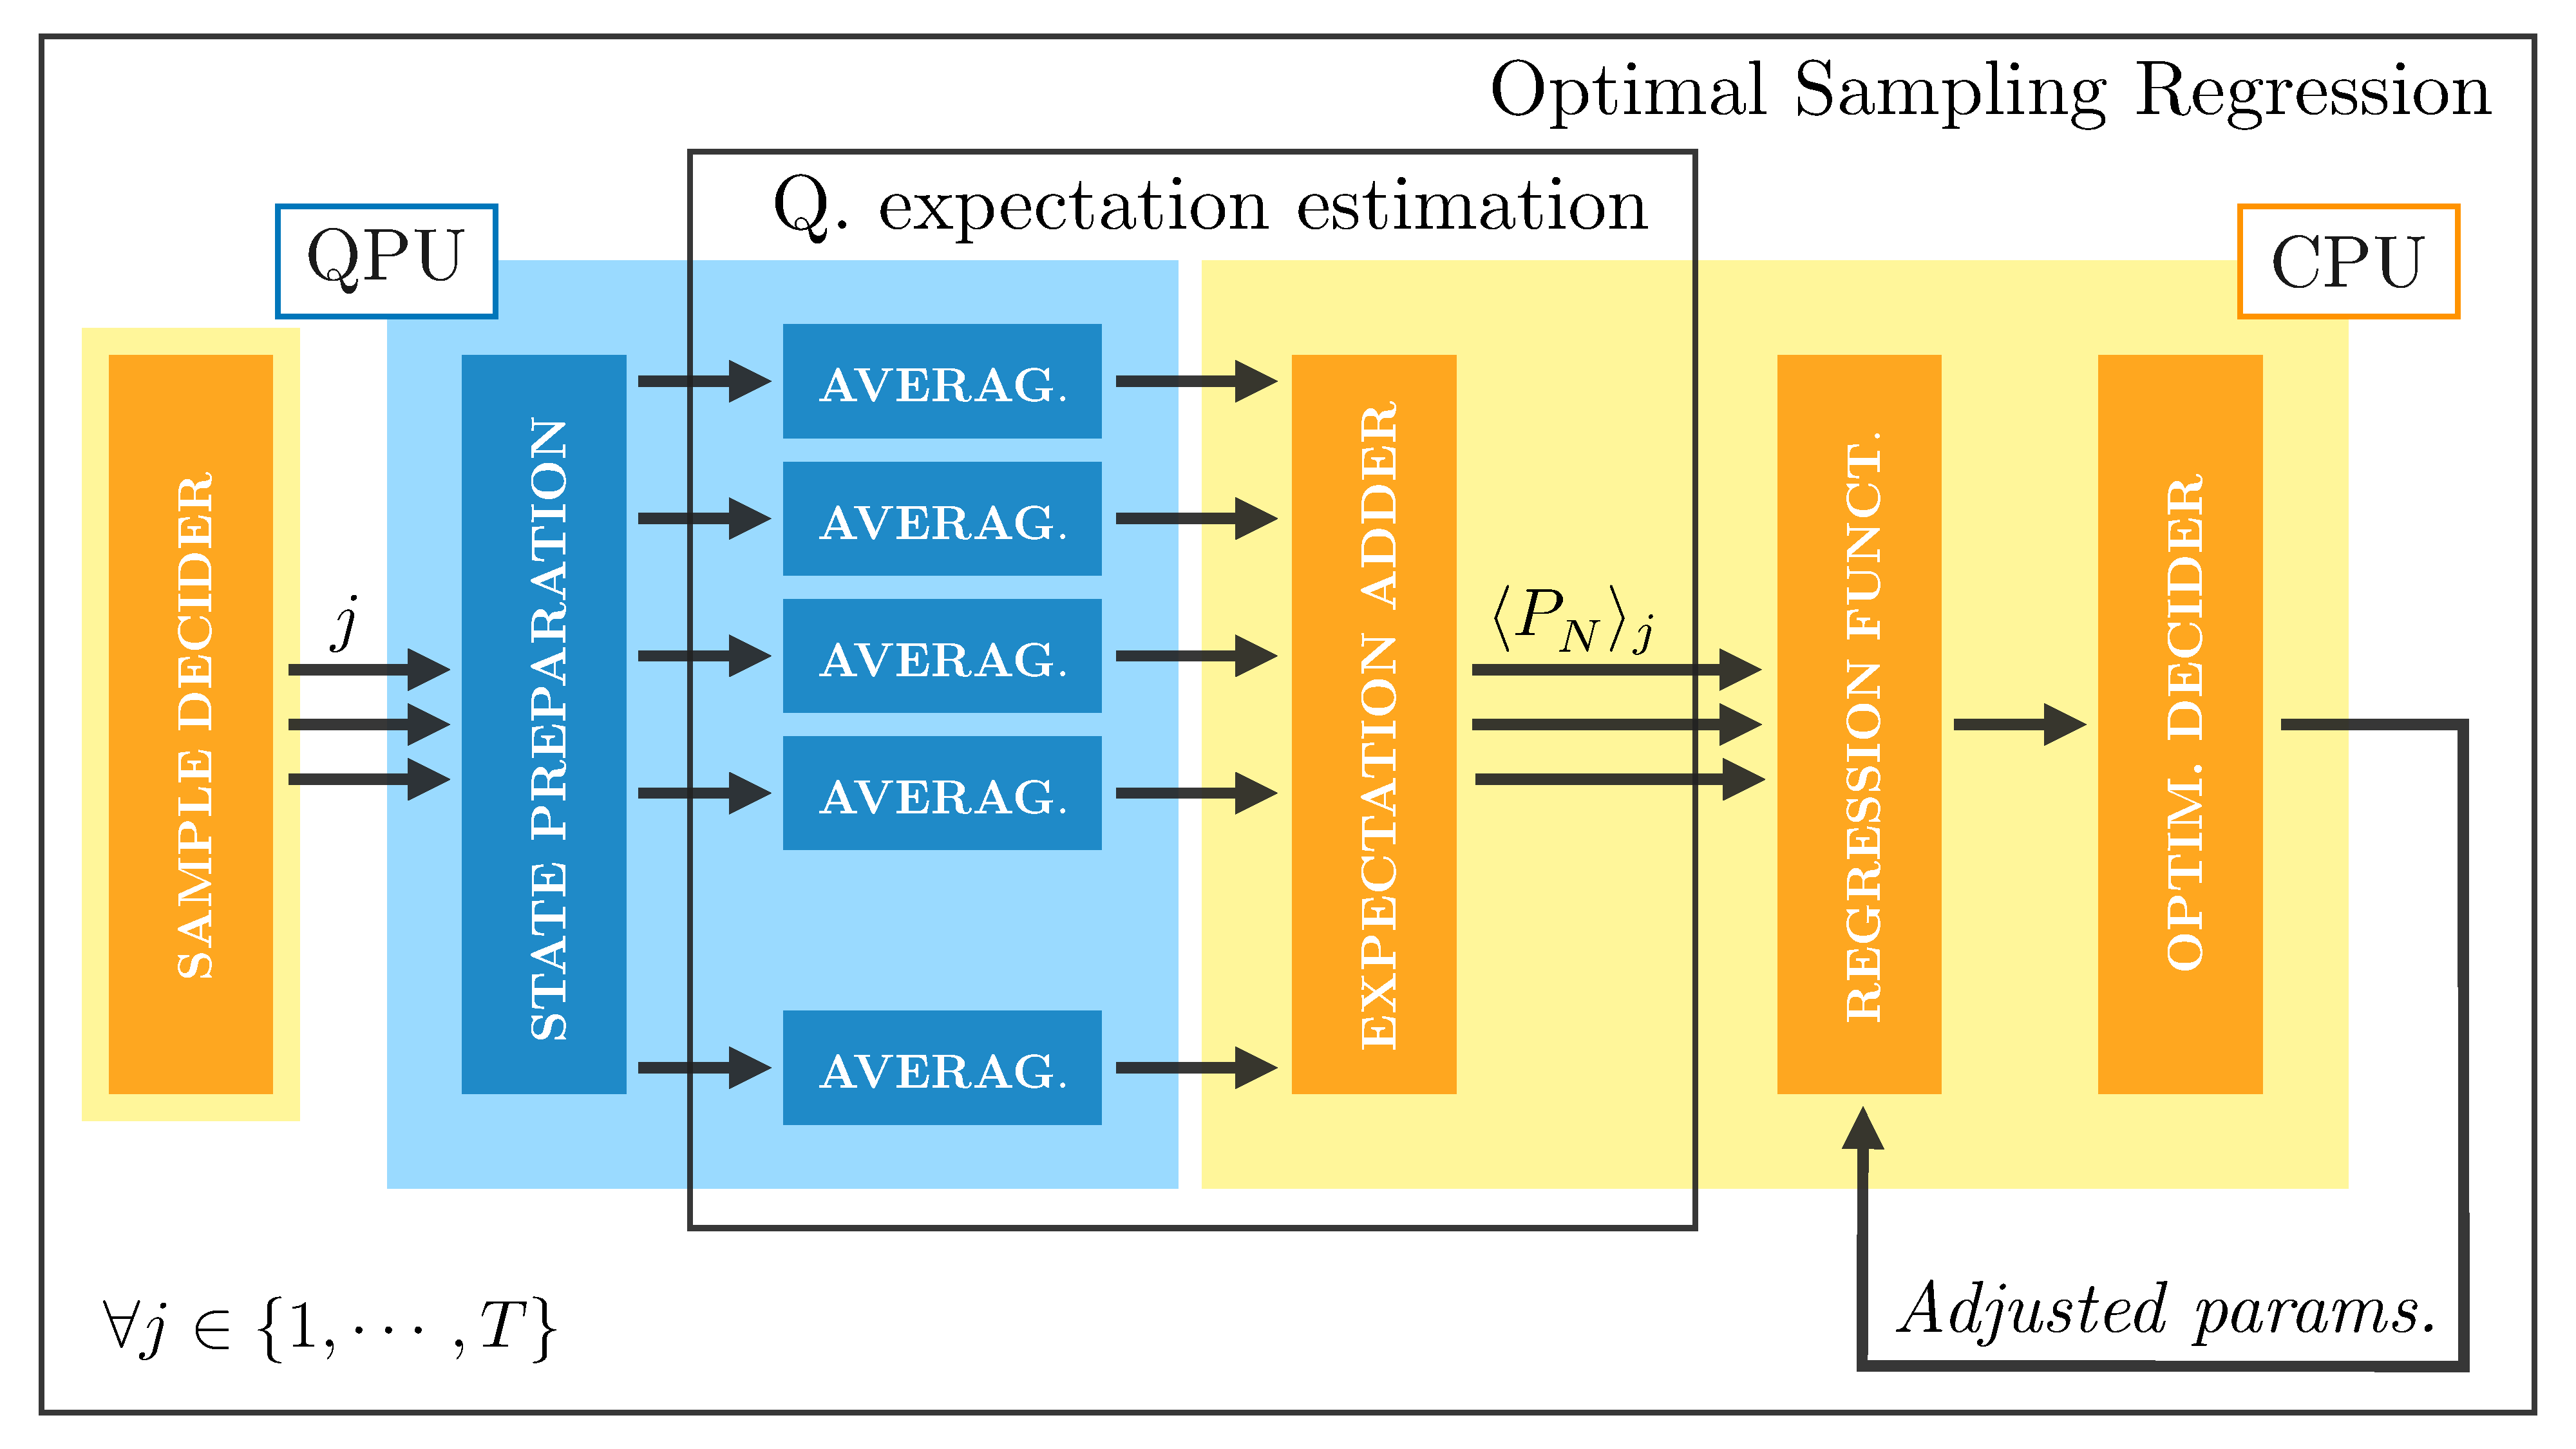
\includegraphics[width=.7\paperwidth]{Figures/NJL1-model-solving/OSR}
	\end{center}

\break

% Overall, what we are fleshing out is a connection between the topology of the quantum circuit and that of the domain space in our parametrization.

\begin{figure}[!tbp]
	\centering
	\begin{minipage}[c]{.40\linewidth}
		\centering
		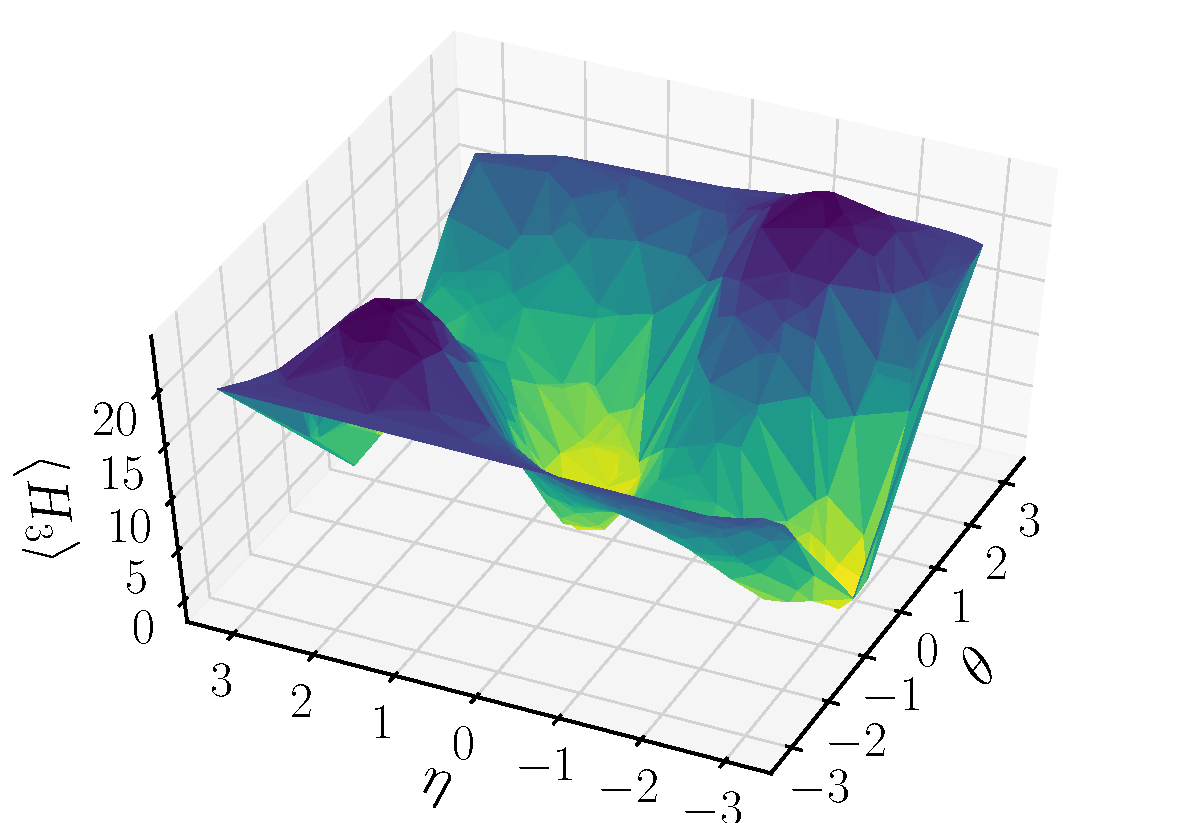
\includegraphics[width=\linewidth]{Figures/NJL1-model-solving/deuteron-VQE}
	\end{minipage}
	\hspace{.025\linewidth}
	\begin{minipage}[c]{.40\linewidth}
		\centering
		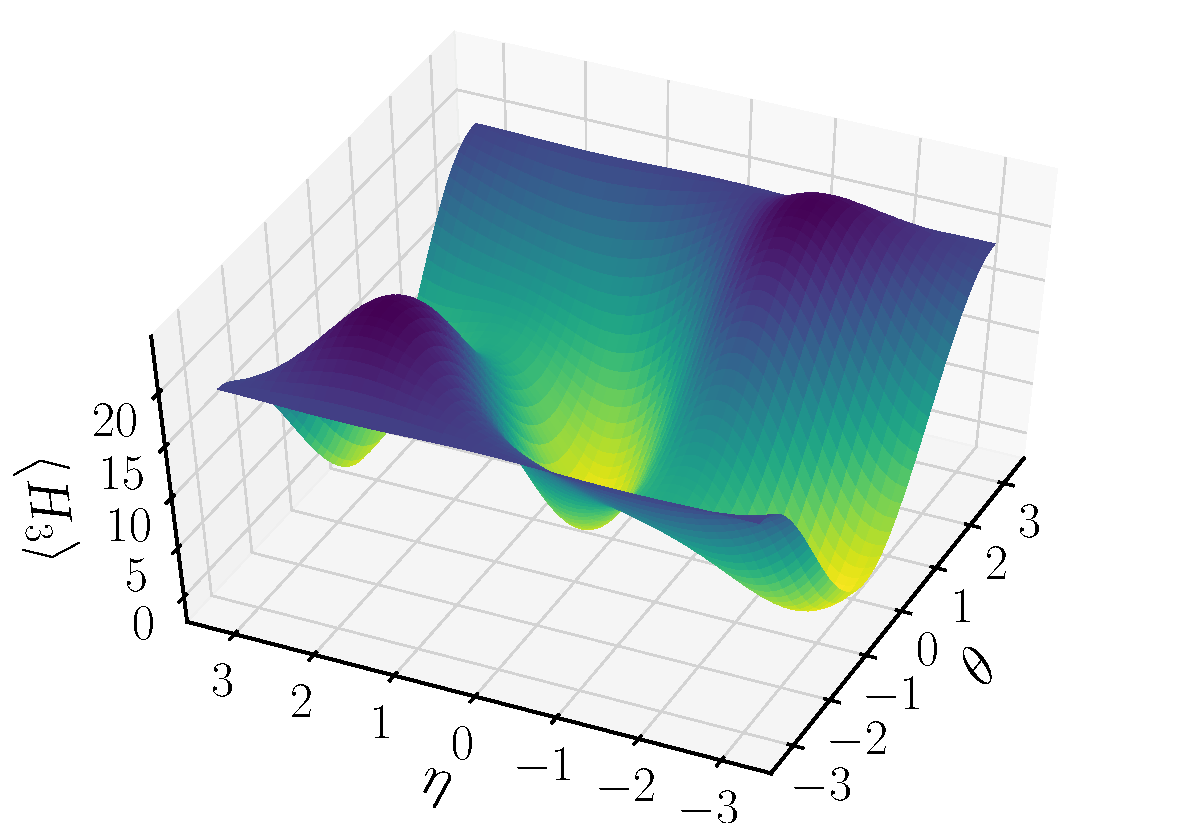
\includegraphics[width=\linewidth]{Figures/NJL1-model-solving/deuteron-OSR}
	\end{minipage}
	\caption{Comparison between the VQE and OSR algorithms, when reproducing an external model with two parameters. (Left) Triangulation of the expectation value function from raw samples. (Right) Approximate function obtained through the Optimal Sampling Regression method with $S_q=S_{\text{max}}=2 ~\forall q$.}
\end{figure}

\vspace{-1em}

\begin{table}[!bp]
	\centering
	% \caption{Comparison between results using the VQE and OSR algorithms.}
	\begin{tabular}{ c c c c c }
		\hline
		% \rule{0pt}{14pt}
		$N_\text{params}$ & VQE samples & OSR samples &
		VQE error & OSR error \\
		\hline
		\hline
		% \rule{0pt}{14pt}
		$1$ & $24$ & $3$ & $3.5\%$ & $1.0\%$ \\
		\hline
		$2$ & $153$ & $25$ & $0.3\%$ & $0.2\%$ \\
		\hline
	\end{tabular}
\end{table}

\end{frame}

%% ----------------------------------------------------------------------------

\begin{frame}[allowframebreaks]{Ground state energy}

	At long last, we have everything that we need to solve for the ground state energy of our system using a quantum computer. For simplicity, we will do so first through a \textbf{quantum simulator}.

	\begin{center}
		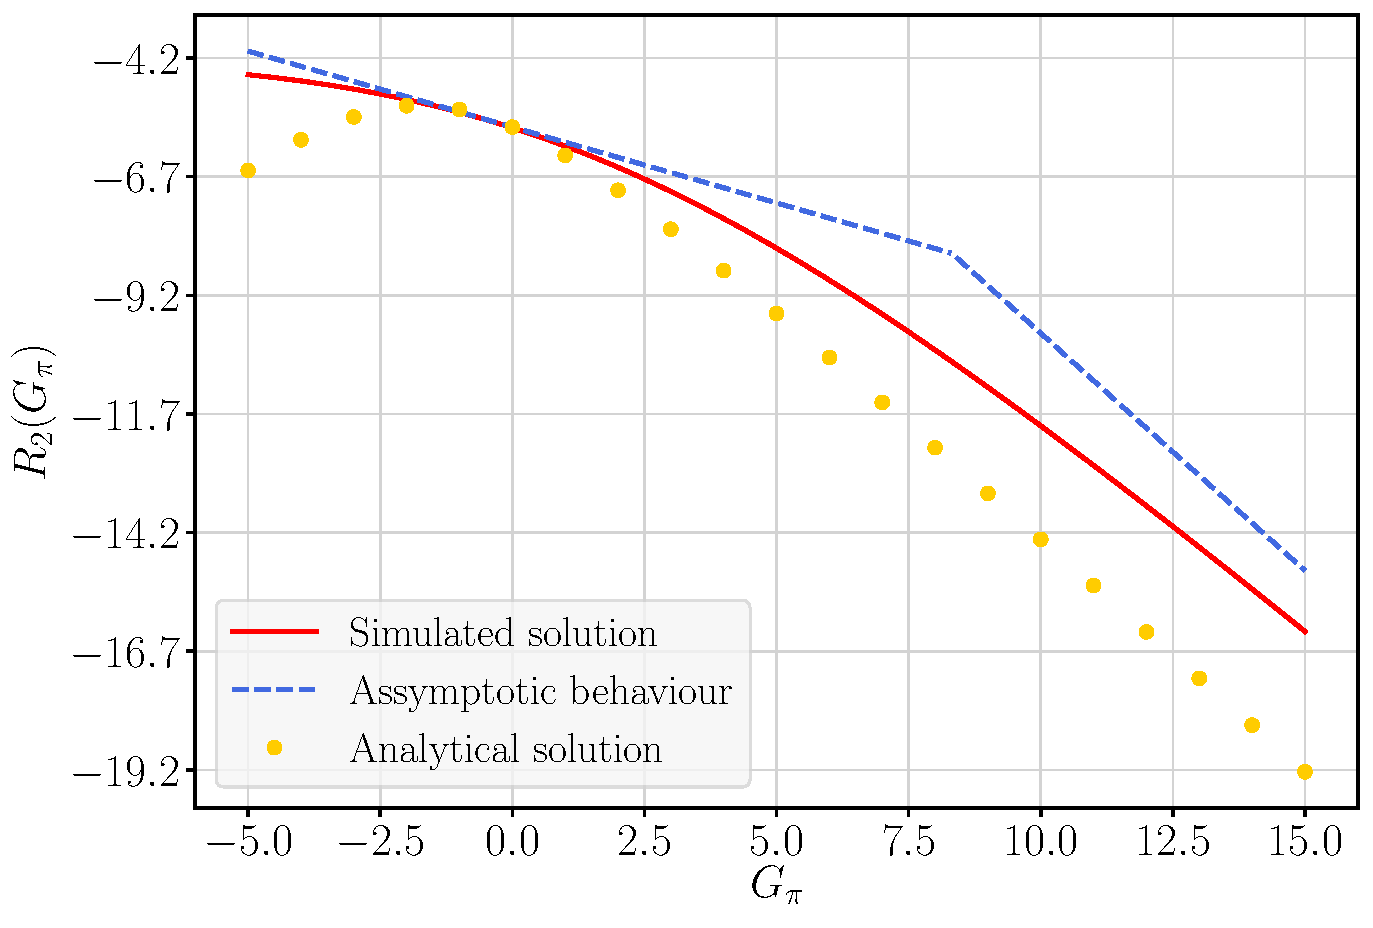
\includegraphics[width=.45\paperwidth]{Figures/NJL1-model-solving/G2}
	\end{center}
	\vspace{-2em}

\break

	\begin{figure}[!p]
		\centering
		\begin{minipage}[c]{.4\linewidth}
			\centering
			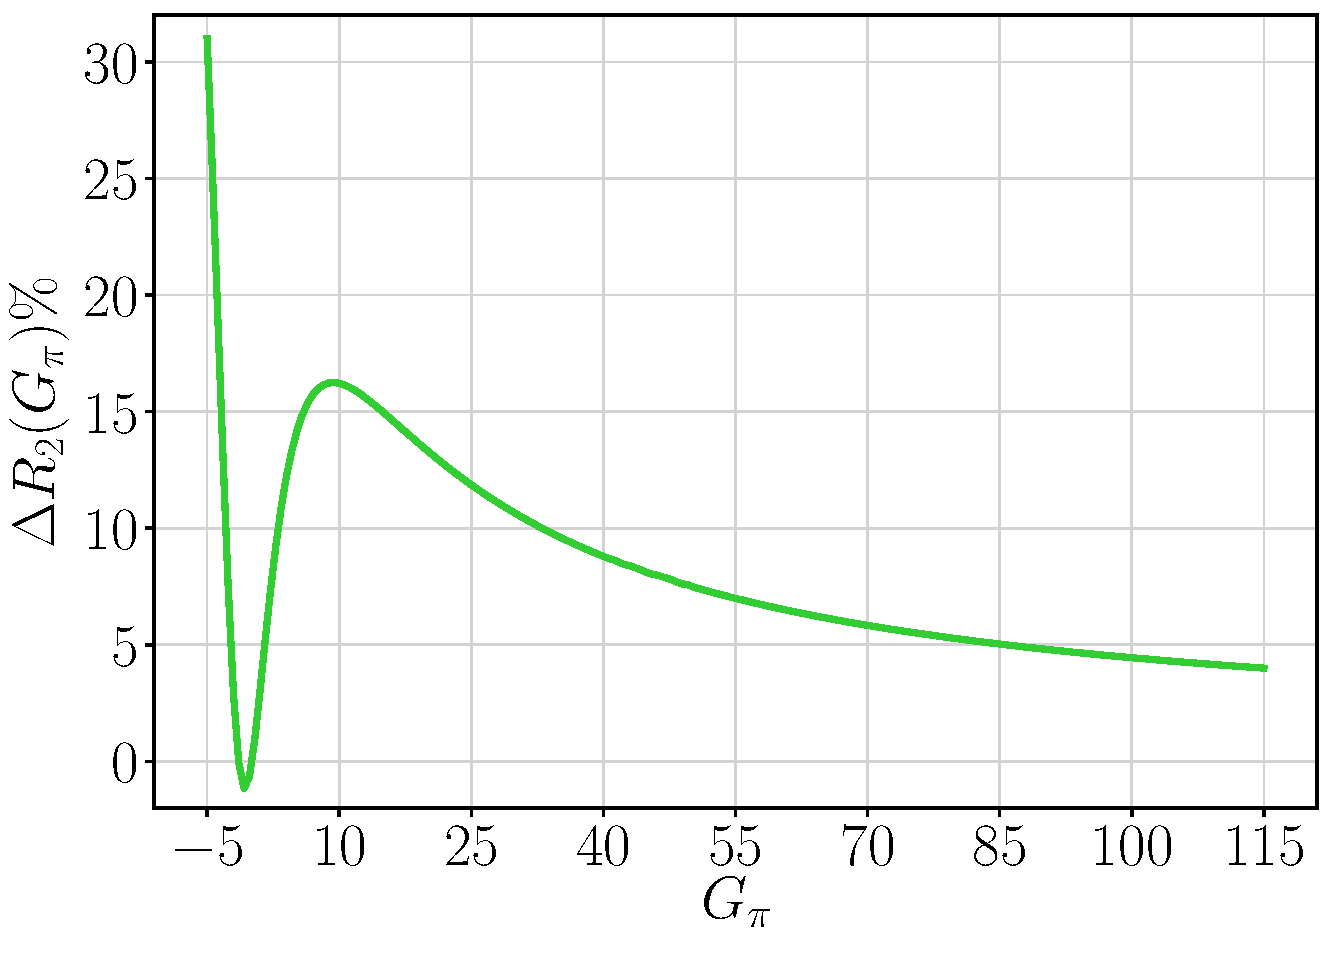
\includegraphics[width=.8\linewidth]{Figures/NJL1-model-solving/G2-err}
		\end{minipage}
		\hspace{.025\linewidth}
		\begin{minipage}[c]{.4\linewidth}
			\centering
			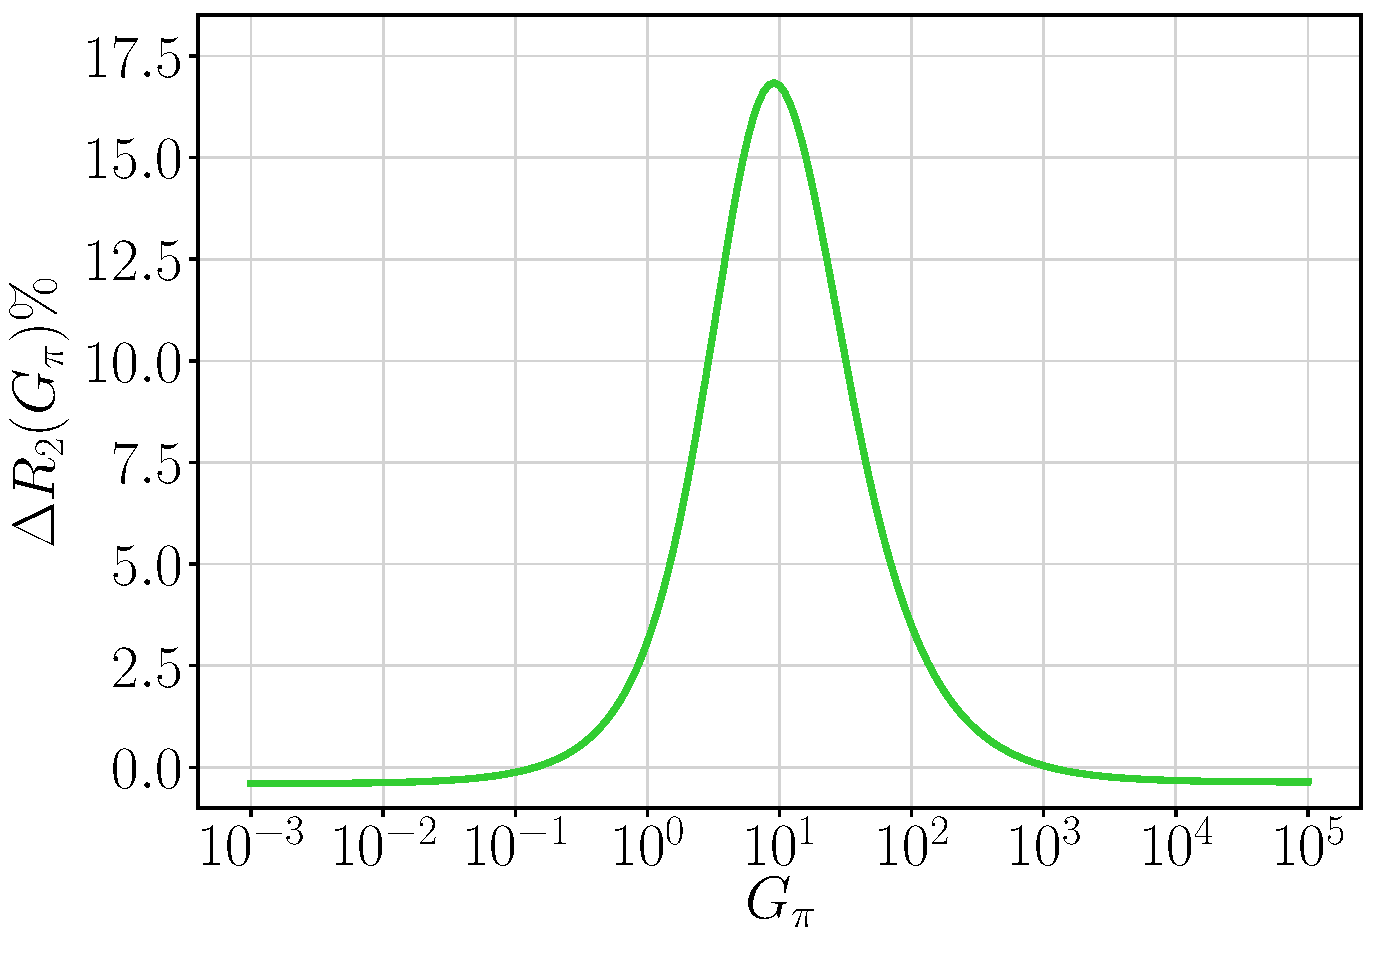
\includegraphics[width=.8\linewidth]{Figures/NJL1-model-solving/G2-logerr}
		\end{minipage} \\[-1em]
		\begin{center}
			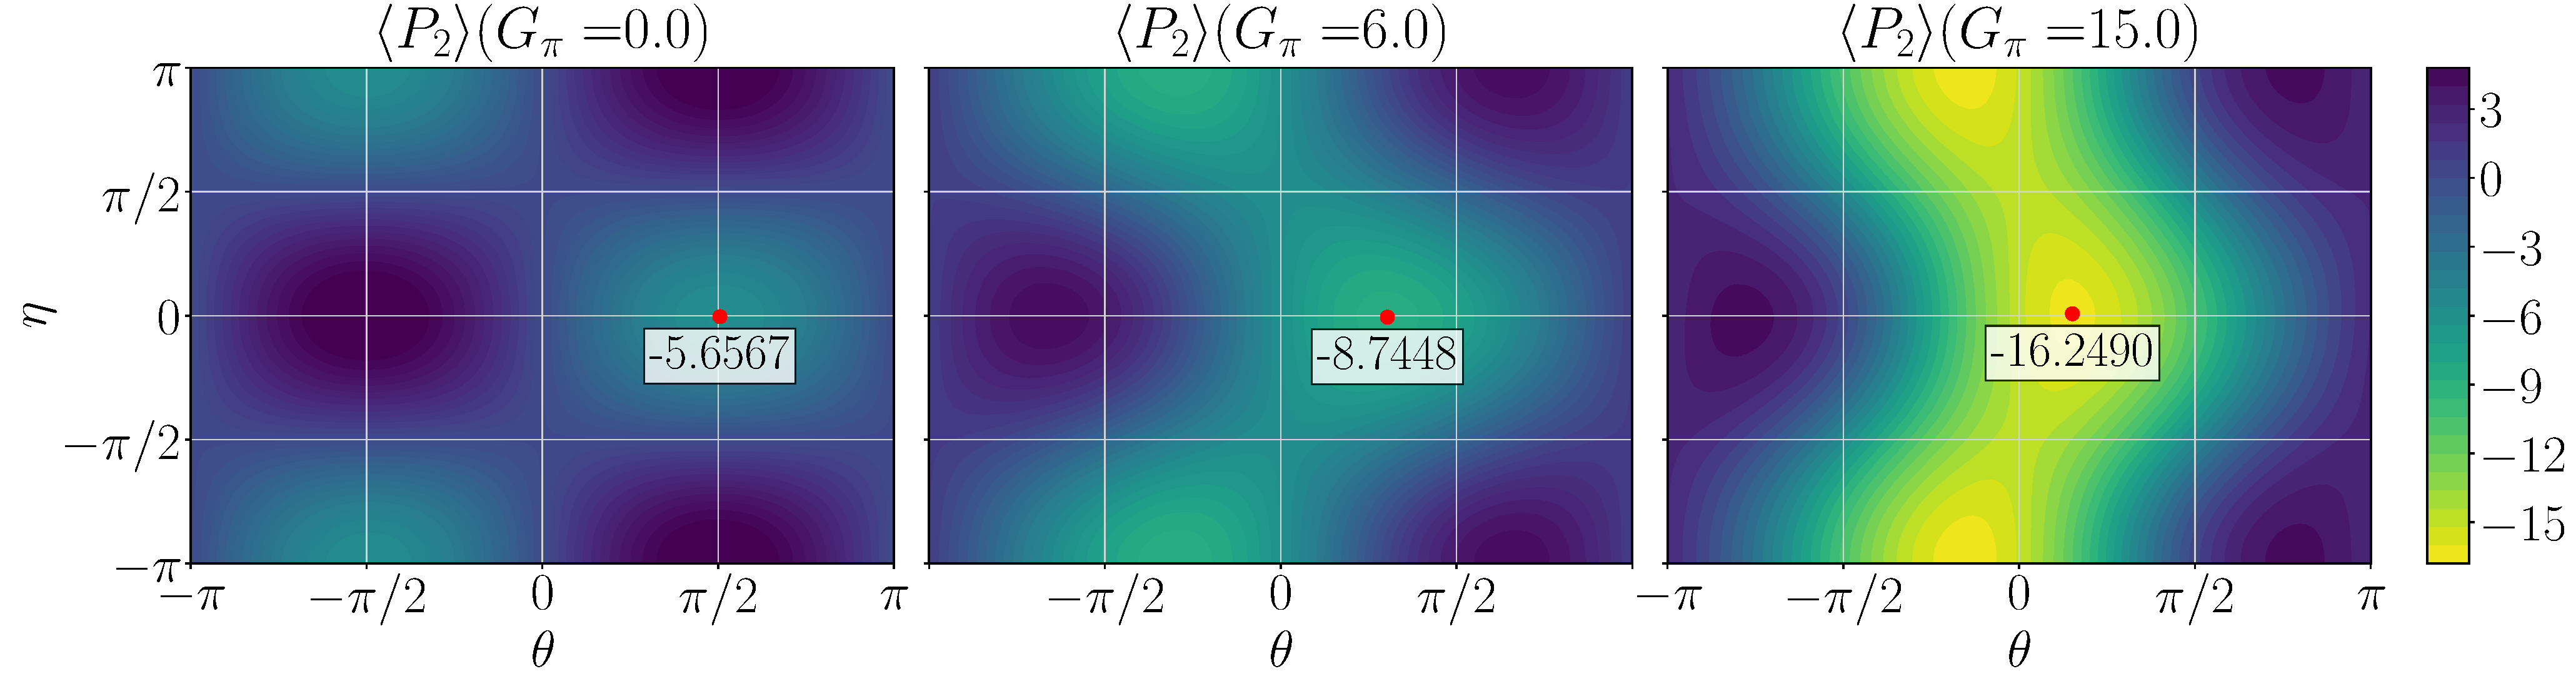
\includegraphics[width=.7\paperwidth]{Figures/NJL1-model-solving/P2-tri-contour}
		\end{center}
		% \caption{Percentual error of the ground state energy results obtained from our quantum simulation with respect to the analytical solution and for different values of the coupling constant. (Left) Linear scale. (Right) Logarithmic scale.}
	\end{figure}
	\vspace{-2em}

\end{frame}

%% ----------------------------------------------------------------------------
%% ----------------------------------------------------------------------------

\section{Conclusions and prospective work}

\begin{frame}{Conlcusions}

	So far I have:

	\begin{itemize}
		\item Reproduced an instance of mass generation in QCD using the NJL model in $1+1$ dimensions, and found the critical value of the coupling constant at which it occurs.
		\item Discretized a simple version of the NJL Hamiltonian using a staggered fermion lattice.
		\item Mapped the resulting Hamultonian onto Pauli operators in order to work with it on a quantum processor.
		\item Developed a custom ansatz for parametrizing certain regions of Hilbert space according to the symmetries of our problem.
		\item Implemented a simplified version of said ansatz as a quantum circuit.
		\item Introduced a new variational algorithm to obtain the minimum eigen value of an encoded operator and tested it against the VQE algorithm.
		\item Used the OSR algorithm to solve for the ground state energy of the NJL Hamiltonian for differernt values of the coupling constant.
	\end{itemize}

\end{frame}

%% ----------------------------------------------------------------------------

\begin{frame}{Prospective work}

	I still have not observed definite evidence of mass generation.

	\medskip

	\begin{itemize}
		\item Implement the full parametrization and compare them with the analytical solution.
		\item Perform these same calculations on actual quantum computers, analyzing any possible differences in the results.
		\item Use a Hamiltonian with two flavors that explicitly contains chiral symmetry, and study properties of the resulting domains (e.g. chiral condensate) such as correlation lengths.
		\item Build a new refactored Hamiltonian which exhibits the finite jumps for arbitrarily small changes in the coupling constant, and backwards engineer a continuum model of QCD.
		\item Study the NJL model in higher dimensions up to full $3+1$ QCD.
		\item Validate the techniques and results.
		\item Describe the scalability of these methods: how fast resource requirements grow once we start increasing the complexity of the systems we are simulating.
		\item Determine some of the limitations of state of the art, as well as short-term NISQ technology.
		\item Develop a consistent notation for these applications of QIS.
	\end{itemize}

\end{frame}


%% ----------------------------------------------------------------------------
%% BACK-MATTER
%% ----------------------------------------------------------------------------

% \section{Bibliography}
% %	\begin{frame}[allowframebreaks]{Bibliography}
% \begin{frame}{Bibliography}
%
% 	\begin{thebibliography}{9}
% 		\setbeamertemplate{bibliography item}[online]
% 	\bibitem{hayden} \textbf{Hayden, P.} \emph{Quantum Computational Universe}
% 		\setbeamertemplate{bibliography item}[book]
% 	\bibitem{susskind_book} \textbf{Susskind, L. \& Friedman A.} \emph{Quantum Mechanics: The Theoretical Minimum}
% 		\setbeamertemplate{bibliography item}[book]
% 	\bibitem{nielsen} \textbf{Nielsen M.A. \& Chuang I.L.} \emph{Quantum Computation and Quantum Information}
% 		\setbeamertemplate{bibliography item}[article]
% 	\bibitem{ladd} \textbf{Lykken J.} \emph{Quantum Technologies for Quantum Science}
% 		\setbeamertemplate{bibliography item}[book]
% 	\bibitem{mermin} \textbf{Mermin N.D.} \emph{Quantum Computer Science: An Introduction}
% 		\setbeamertemplate{bibliography item}[article]
% 	\bibitem{ladd} \textbf{Ladd T.D. (et al.)} \emph{Quantum Computing}
%
% 	\end{thebibliography}
%
% 	\vspace{20pt}
% 	\begin{small}
% 	\begin{center}{
% 	\color{gray}
% 		\emph{"The only thing demonstrated by an impossibility proof is a lack of imagination."} \\
% 		\textbf{– John Stewart Bell –} }
% 	\end{center}
% 	\end{small}
% \end{frame}

%% ----------------------------------------------------------------------------

\FinalFrame

%% ----------------------------------------------------------------------------

\end{document}
